% Options for packages loaded elsewhere
\PassOptionsToPackage{unicode}{hyperref}
\PassOptionsToPackage{hyphens}{url}
%
\documentclass[
]{book}
\usepackage{amsmath,amssymb}
\usepackage{iftex}
\ifPDFTeX
  \usepackage[T1]{fontenc}
  \usepackage[utf8]{inputenc}
  \usepackage{textcomp} % provide euro and other symbols
\else % if luatex or xetex
  \usepackage{unicode-math} % this also loads fontspec
  \defaultfontfeatures{Scale=MatchLowercase}
  \defaultfontfeatures[\rmfamily]{Ligatures=TeX,Scale=1}
\fi
\usepackage{lmodern}
\ifPDFTeX\else
  % xetex/luatex font selection
\fi
% Use upquote if available, for straight quotes in verbatim environments
\IfFileExists{upquote.sty}{\usepackage{upquote}}{}
\IfFileExists{microtype.sty}{% use microtype if available
  \usepackage[]{microtype}
  \UseMicrotypeSet[protrusion]{basicmath} % disable protrusion for tt fonts
}{}
\makeatletter
\@ifundefined{KOMAClassName}{% if non-KOMA class
  \IfFileExists{parskip.sty}{%
    \usepackage{parskip}
  }{% else
    \setlength{\parindent}{0pt}
    \setlength{\parskip}{6pt plus 2pt minus 1pt}}
}{% if KOMA class
  \KOMAoptions{parskip=half}}
\makeatother
\usepackage{xcolor}
\usepackage{color}
\usepackage{fancyvrb}
\newcommand{\VerbBar}{|}
\newcommand{\VERB}{\Verb[commandchars=\\\{\}]}
\DefineVerbatimEnvironment{Highlighting}{Verbatim}{commandchars=\\\{\}}
% Add ',fontsize=\small' for more characters per line
\usepackage{framed}
\definecolor{shadecolor}{RGB}{248,248,248}
\newenvironment{Shaded}{\begin{snugshade}}{\end{snugshade}}
\newcommand{\AlertTok}[1]{\textcolor[rgb]{0.94,0.16,0.16}{#1}}
\newcommand{\AnnotationTok}[1]{\textcolor[rgb]{0.56,0.35,0.01}{\textbf{\textit{#1}}}}
\newcommand{\AttributeTok}[1]{\textcolor[rgb]{0.13,0.29,0.53}{#1}}
\newcommand{\BaseNTok}[1]{\textcolor[rgb]{0.00,0.00,0.81}{#1}}
\newcommand{\BuiltInTok}[1]{#1}
\newcommand{\CharTok}[1]{\textcolor[rgb]{0.31,0.60,0.02}{#1}}
\newcommand{\CommentTok}[1]{\textcolor[rgb]{0.56,0.35,0.01}{\textit{#1}}}
\newcommand{\CommentVarTok}[1]{\textcolor[rgb]{0.56,0.35,0.01}{\textbf{\textit{#1}}}}
\newcommand{\ConstantTok}[1]{\textcolor[rgb]{0.56,0.35,0.01}{#1}}
\newcommand{\ControlFlowTok}[1]{\textcolor[rgb]{0.13,0.29,0.53}{\textbf{#1}}}
\newcommand{\DataTypeTok}[1]{\textcolor[rgb]{0.13,0.29,0.53}{#1}}
\newcommand{\DecValTok}[1]{\textcolor[rgb]{0.00,0.00,0.81}{#1}}
\newcommand{\DocumentationTok}[1]{\textcolor[rgb]{0.56,0.35,0.01}{\textbf{\textit{#1}}}}
\newcommand{\ErrorTok}[1]{\textcolor[rgb]{0.64,0.00,0.00}{\textbf{#1}}}
\newcommand{\ExtensionTok}[1]{#1}
\newcommand{\FloatTok}[1]{\textcolor[rgb]{0.00,0.00,0.81}{#1}}
\newcommand{\FunctionTok}[1]{\textcolor[rgb]{0.13,0.29,0.53}{\textbf{#1}}}
\newcommand{\ImportTok}[1]{#1}
\newcommand{\InformationTok}[1]{\textcolor[rgb]{0.56,0.35,0.01}{\textbf{\textit{#1}}}}
\newcommand{\KeywordTok}[1]{\textcolor[rgb]{0.13,0.29,0.53}{\textbf{#1}}}
\newcommand{\NormalTok}[1]{#1}
\newcommand{\OperatorTok}[1]{\textcolor[rgb]{0.81,0.36,0.00}{\textbf{#1}}}
\newcommand{\OtherTok}[1]{\textcolor[rgb]{0.56,0.35,0.01}{#1}}
\newcommand{\PreprocessorTok}[1]{\textcolor[rgb]{0.56,0.35,0.01}{\textit{#1}}}
\newcommand{\RegionMarkerTok}[1]{#1}
\newcommand{\SpecialCharTok}[1]{\textcolor[rgb]{0.81,0.36,0.00}{\textbf{#1}}}
\newcommand{\SpecialStringTok}[1]{\textcolor[rgb]{0.31,0.60,0.02}{#1}}
\newcommand{\StringTok}[1]{\textcolor[rgb]{0.31,0.60,0.02}{#1}}
\newcommand{\VariableTok}[1]{\textcolor[rgb]{0.00,0.00,0.00}{#1}}
\newcommand{\VerbatimStringTok}[1]{\textcolor[rgb]{0.31,0.60,0.02}{#1}}
\newcommand{\WarningTok}[1]{\textcolor[rgb]{0.56,0.35,0.01}{\textbf{\textit{#1}}}}
\usepackage{longtable,booktabs,array}
\usepackage{calc} % for calculating minipage widths
% Correct order of tables after \paragraph or \subparagraph
\usepackage{etoolbox}
\makeatletter
\patchcmd\longtable{\par}{\if@noskipsec\mbox{}\fi\par}{}{}
\makeatother
% Allow footnotes in longtable head/foot
\IfFileExists{footnotehyper.sty}{\usepackage{footnotehyper}}{\usepackage{footnote}}
\makesavenoteenv{longtable}
\usepackage{graphicx}
\makeatletter
\def\maxwidth{\ifdim\Gin@nat@width>\linewidth\linewidth\else\Gin@nat@width\fi}
\def\maxheight{\ifdim\Gin@nat@height>\textheight\textheight\else\Gin@nat@height\fi}
\makeatother
% Scale images if necessary, so that they will not overflow the page
% margins by default, and it is still possible to overwrite the defaults
% using explicit options in \includegraphics[width, height, ...]{}
\setkeys{Gin}{width=\maxwidth,height=\maxheight,keepaspectratio}
% Set default figure placement to htbp
\makeatletter
\def\fps@figure{htbp}
\makeatother
\setlength{\emergencystretch}{3em} % prevent overfull lines
\providecommand{\tightlist}{%
  \setlength{\itemsep}{0pt}\setlength{\parskip}{0pt}}
\setcounter{secnumdepth}{5}
\usepackage{booktabs}
\ifLuaTeX
  \usepackage{selnolig}  % disable illegal ligatures
\fi
\usepackage[]{natbib}
\bibliographystyle{plainnat}
\IfFileExists{bookmark.sty}{\usepackage{bookmark}}{\usepackage{hyperref}}
\IfFileExists{xurl.sty}{\usepackage{xurl}}{} % add URL line breaks if available
\urlstyle{same}
\hypersetup{
  pdftitle={R for social science and business analytics},
  pdfauthor={Raffaele Vacca},
  hidelinks,
  pdfcreator={LaTeX via pandoc}}

\title{R for social science and business analytics}
\author{\href{http://www.raffaelevacca.com/}{Raffaele Vacca}}
\date{2024-06-10}

\begin{document}
\maketitle

{
\setcounter{tocdepth}{1}
\tableofcontents
}
\hypertarget{overview-and-setup}{%
\chapter{Overview and setup}\label{overview-and-setup}}

This is a series of four workshop sessions about R programming for social science research and business analytics:

\begin{enumerate}
\def\labelenumi{\arabic{enumi}.}
\tightlist
\item
  \protect\hyperlink{intro}{Introduction to R} (\texttt{01\_basics.R} script): R objects, vectors and matrices, arithmetic and logical operations, subsetting and indexing, data frames and lists, R functions.
\item
  \protect\hyperlink{wrangling}{Data wrangling and descriptive statistics} (\texttt{02\_wrangling.R} script): importing data, subsetting, ordering cases and variables, transforming and recoding, joining and appending data frames; frequency tables and crosstabs, mean, standard deviation and other descriptive functions, descriptive statistics for data subsets.
\item
  \protect\hyperlink{visualization}{Data visualization} (\texttt{03\_visualization.R} script): the ggplot2 package and the grammar of graphics, geometries and aesthetics, visualizing univariate distributions (histograms, boxplots, simple bar plots etc.), Visualizing associations between two or more variables (scatterplots, complex bar plots, etc.).
\item
  \protect\hyperlink{reproducible}{Creating reproducible reports} (\texttt{04\_reports.R} script): reproducible reports in different formats, RMarkdown basics, R code chunks, chunk options, inline R code.
\end{enumerate}

\hypertarget{setup}{%
\section{Workshop setup}\label{setup}}

To take this workshop you need to:

\begin{enumerate}
\def\labelenumi{\arabic{enumi}.}
\tightlist
\item
  Download the last version of \textbf{R} \href{https://cran.r-project.org/mirrors.html}{here}

  \begin{itemize}
  \tightlist
  \item
    Select a location near you in the web page above
  \item
    Follow instructions to install R on your computer
  \end{itemize}
\item
  Download \textbf{RStudio} (free version) \href{https://www.rstudio.com/products/rstudio/download/}{here}

  \begin{itemize}
  \tightlist
  \item
    Follow instructions to install RStudio on your computer
  \end{itemize}
\item
  Bring your \textbf{laptop} to the workshop
\item
  Download the \textbf{workshop folder} and save it to your computer: see \protect\hyperlink{materials}{below}

  \begin{itemize}
  \tightlist
  \item
    I recommend that you do this in class at the beginning of the workshop so as to download the most updated version of the folder.
  \end{itemize}
\item
  Once in class, go to the workshop folder on your computer (point 4 above) and double-click on the \textbf{R project} file in it (\texttt{.Rproj} extension).

  \begin{itemize}
  \tightlist
  \item
    That will open RStudio: you're all set!
  \end{itemize}
\end{enumerate}

\textbf{NOTE:} It's very important that you save the workshop folder \emph{as downloaded} to a location in your computer, and open the \texttt{.Rproj} \emph{within that folder}. By doing so, you will be opening RStudio \emph{and} setting the workshop folder as your \protect\hyperlink{starting-R-and-loading-packages}{R working directory}. All our R scripts assume the workshop folder is your working directory. You can type \texttt{getwd()} in your R console to see the path to your R working directory and make sure that it's correctly pointing to the location of the workshop folder in your computer.

\hypertarget{materials}{%
\section{Workshop materials}\label{materials}}

The materials for this workshop consist of this website and the workshop folder.

You can \textbf{download} the workshop folder from \href{https://github.com/raffaelevacca/r-social-business-analytics}{this GitHub repository}:

\begin{enumerate}
\def\labelenumi{\arabic{enumi}.}
\tightlist
\item
  Click on the \emph{Code} green button \textgreater{} Download ZIP
\item
  Unzip the folder and save it to your computer
\end{enumerate}

The workshop folder contains several files and subfolders, but you only need to focus on the following:

\begin{itemize}
\tightlist
\item
  \texttt{scripts} subfolder: all the R code shown in this website.
\item
  \texttt{data} subfolder: all the data we're going to use.
\item
  \texttt{r-social-business-analytics.Rproj}: the workshop's R project file (you use this to launch RStudio).
\end{itemize}

The \texttt{scripts} subfolder includes different R script (.R) files. You can access and run the R code in each script by opening that .R file in RStudio.

\hypertarget{r-settings}{%
\section{R settings}\label{r-settings}}

\hypertarget{packages}{%
\subsection{Required R packages}\label{packages}}

We'll install and load these in class:

\begin{itemize}
\tightlist
\item
  \href{https://cran.r-project.org/web/packages/janitor/vignettes/janitor.html}{\texttt{janitor}}
\item
  \href{https://cran.r-project.org/web/packages/skimr/vignettes/skimr.html}{\texttt{skimr}}
\item
  \href{https://www.tidyverse.org/}{\texttt{tidyverse}}
\end{itemize}

The tidyverse isn't a single package, it's a collection of packages that share a common set of functions and principles, including \texttt{dplyr}, \texttt{ggplot2}, and \texttt{purrr}. See the \href{https://www.tidyverse.org/}{tidyverse website} for more information.

\hypertarget{rstudio-options}{%
\subsection{RStudio options}\label{rstudio-options}}

RStudio gives you the ability to select and change various settings and features of its interface: see the \texttt{Preferences...} menu option.

These are some of the settings you should pay attention to:

\begin{itemize}
\tightlist
\item
  \texttt{Preferences...\ \textgreater{}\ Code\ \textgreater{}\ Editing\ \textgreater{}\ Soft-wrap\ R\ source\ file}. Here you can decide whether or not to wrap long code lines in the editor. When code lines in a script are \emph{not} wrapped, some code will be hidden if script lines are longer than your editor window's width (you'll have to scroll right to see the rest of the code). With a script open in the editor, try both options (checked and unchecked) to see what you're more comfortable with.
\item
  \texttt{Preferences...\ \textgreater{}\ Code\ \textgreater{}\ Display\ \textgreater{}\ Highlight\ R\ function\ calls}. This allows you to highlight all pieces of code that call an R function (``command''). I find function highlights very helpful to navigate a script and suggest that you check this option.
\end{itemize}

\hypertarget{data}{%
\section{Data}\label{data}}

This workshop uses an anonymized subset of the survey data collected for Valore D's \href{https://www.valored.it/ricerche/oltre-le-generazioni-esperienze-relazioni-lavoro/}{Oltre le generazioni} study, limited to 1000 randomly selected cases (survey respondents, i.e.~employees) and with fictitious company names. All data are in the \texttt{data} subfolder.

\hypertarget{author-and-contacts}{%
\section{Author and contacts}\label{author-and-contacts}}

I'm an assistant professor of sociology at the \href{https://www.unimi.it/en}{University of Milan} in the \href{http://eng.sps.unimi.it/ecm/home}{Deparment of Social and Political Sciences} and its \href{https://behavelab.org/}{Behave Lab}. My main research and teaching interests are social networks, migration, health inequalities, and studies of science. I also teach and do research on data science, statistics, and computational methods for the social sciences. More information about me, my work and my contact details is \href{http://www.raffaelevacca.com/}{here}.

\begin{Shaded}
\begin{Highlighting}[]
\FunctionTok{library}\NormalTok{(knitr)}
\CommentTok{\# Copy all R code to separate R files.}
\NormalTok{knitr}\SpecialCharTok{::}\FunctionTok{purl}\NormalTok{(}\AttributeTok{input =} \StringTok{"03\_data{-}wrangling{-}descriptive.Rmd"}\NormalTok{,}
            \AttributeTok{output =} \StringTok{"./scripts/02\_wrangling.R"}\NormalTok{)}
\NormalTok{knitr}\SpecialCharTok{::}\FunctionTok{purl}\NormalTok{(}\AttributeTok{input =} \StringTok{"04\_data{-}viz.Rmd"}\NormalTok{,}
            \AttributeTok{output =} \StringTok{"./scripts/03\_visualization.R"}\NormalTok{)}
\end{Highlighting}
\end{Shaded}

\hypertarget{intro}{%
\chapter{Introduction to R}\label{intro}}

The script covers the following topics:

\begin{itemize}
\tightlist
\item
  Starting R, getting help with R.
\item
  Creating and saving R objects.
\item
  Vectors and matrices, data frames and tibbles.
\item
  Arithmetic and relational operations.
\item
  Subsetting vectors, matrices, and data frames.
\item
  Pipes and the pipe operator.
\item
  Object types and classes.
\item
  Writing R functions.
\end{itemize}

\hypertarget{starting-R-and-loading-packages}{%
\section{Starting R and loading packages}\label{starting-R-and-loading-packages}}

\begin{itemize}
\tightlist
\item
  Before starting any work in R, you normally want to do two things:

  \begin{itemize}
  \tightlist
  \item
    Make sure your R session is pointing to the correct \emph{working directory}.
  \item
    Install and/or load the \emph{packages} you are going to use.
  \end{itemize}
\item
  \textbf{Working directory}. By default, R will look for files and save new files in this directory.

  \begin{itemize}
  \tightlist
  \item
    Type \texttt{getwd()} in the console to view your current working directory.
  \item
    If you opened RStudio by double-clicking on a project (\texttt{.Rproj}) file, then the working directory is the folder where that file is located.
  \item
    You can always use \texttt{setwd()} to manually change your working directory to any path, but it's usually more convenient to work with R projects and their default working directory instead.
  \item
    In RStudio, you can also check the current working directory by clicking on the \texttt{Files} panel.
  \end{itemize}
\item
  \textbf{R packages}. There are two steps to using a package in R:

  \begin{enumerate}
  \def\labelenumi{\arabic{enumi}.}
  \tightlist
  \item
    \textbf{Install} the package. \emph{You do this just once}. Use \texttt{install.packages("package\_name")} or the appropriate RStudio menu (\texttt{Tools\ \textgreater{}\ Install\ Packages...}). Once you install a package, the package files are in your system R folder and R will be able to always find the package there.
  \item
    \textbf{Load} the package in your current session. Use \texttt{library(package\_name)} (\emph{no} quotation marks around the package name). \emph{You do this in each R session in which you need the package}, that is, every time you start R and you need the package.
  \end{enumerate}
\item
  An R package is just a collection of \textbf{functions}. You can only use an R function if that function is included in a package you loaded in the current session.
\item
  Sometimes two different functions from two different packages have the same \textbf{name}. For example, both the \texttt{igraph} package and the \texttt{sna} package have a function called \texttt{degree}. If both packages are loaded, typing just \texttt{degree} might give you unexpected results, because R will pick one of the two functions (the one in the package that was loaded most recently), which might not be the function you meant.

  \begin{itemize}
  \tightlist
  \item
    To avoid this problem, you can use the \texttt{package::function()} notation: \texttt{igraph::degree()} will always call the \texttt{degree} function from the \texttt{igraph} package, while \texttt{sna::degree()} will call the \texttt{degree} function from the \texttt{sna} package.
  \end{itemize}
\item
  Tip: To check the package that a function comes from, just go to that function's manual page. The package will be indicated in the first line of the page. E.g., type \texttt{?degree} to see where the \texttt{degree} function comes from.

  \begin{itemize}
  \tightlist
  \item
    If no currently loaded package has a function called \texttt{degree}, then typing \texttt{?degree} will produce a warning (\texttt{No\ documentation\ for\ \textquotesingle{}degree\textquotesingle{}}).
  \item
    If multiple, currently loaded packages have a function called \texttt{degree}, then typing \texttt{?degree} will bring up a page with the list of all those packages.
  \end{itemize}
\item
  This workshop will use different packages, listed \protect\hyperlink{packages}{here}.
\end{itemize}

\hypertarget{console-vs-scripts}{%
\subsection{Console vs scripts}\label{console-vs-scripts}}

\begin{itemize}
\tightlist
\item
  When you open RStudio, you typically see two separate panels: the script editor and the console. You can write R code in either of them.
\item
  \textbf{Console}. Here you write R code line by line. Once you type a line, you press \texttt{ENTER} to execute it. By pressing \texttt{ARROW\ UP} you go back to the last line you ran. By continuing to press \texttt{ARROW\ UP}, you can navigate through all the lines of code you previously executed. This is called the ``commands history'' (all the lines of code executed in the current session). You will lose all this code (all the history) when you quit R, unless you explicitly save the history to a file (which is not what you typically do, you should just write the code in a script).\\
\item
  \textbf{Script editor}. Here you write a script. This is the most common way of working with R. A script is simply a plain text file where all your R code is saved. If your work is in a script, it is \textbf{reproducible}.
\item
  Both the R standard GUI and RStudio have a script editor with several helpful tools. Among other things, these allow you to run a script while you write it. By pressing \texttt{CTRL+ENTER} (Windows) or \texttt{CMD+ENTER} (Mac), you run the script line your cursor is on (or the selected script region).

  \begin{itemize}
  \tightlist
  \item
    Note that with RStudio you can run the single script line where your cursor is; a whole highlighted region of code; the region of code from the beginning of the script up to the line where your cursor is; the region of code from the line where your cursor is up to the end of the script. See the \emph{Code} menu and its keyboard shortcuts.
  \end{itemize}
\item
  The script editor also allows you to save your script. In RStudio, see \texttt{File\ \textgreater{}\ Save} and its keyboard shortcut. R script files commonly have a \texttt{.R} extension (e.g.~``\texttt{myscript.R}''). But note that a script file is just a text file (like any \texttt{.txt} file), which you can open and edit in any text editor, or in Microsoft Word and the likes.
\item
  You can also run a whole script altogether --- this is called \textbf{sourcing} a script. By running \texttt{source("myscript.R")}, you source the script file \texttt{myscript.R} (assuming the file is in your working directory, otherwise you'll have to enter the whole file path). In RStudio: see \emph{Code} \textgreater{} \emph{Source} and its keyboard shortcut.
\item
  In both the console and the script editor, any line that starts by \texttt{\#} is called a \textbf{comment}. R disregards comments --- it just prints them as they are in the console (does not parse and execute them as programming code). Remember to always use comments to document what your code is doing (this is good for yourself and for others).
\item
  In RStudio you can navigate the script headings in your script with a drop-down menu in the bottom-left of the script editor. Any line that starts by \texttt{\#} and ends by \texttt{\#\#\#\#}, \texttt{-\/-\/-\/-}, or \texttt{====} is read as a heading by RStudio.
\end{itemize}

\hypertarget{getting-help}{%
\subsection{Getting help}\label{getting-help}}

\begin{itemize}
\tightlist
\item
  Getting help is one of the most common things you do when using R. As a beginner, you'll constantly need to get help (for example, read manual pages) about R functions. Also as an experienced user, you'll often need to go back to the manual pages of particular functions or other R help resources. At any experience level, using R involves constantly using its documentation and help resources.
\item
  The following are a few help tools in R:

  \begin{itemize}
  \tightlist
  \item
    \texttt{help(...)} or \texttt{?...} are the most common ways of getting help: they send you to the R manual page for a specific function. E.g. \texttt{help(sum)} or \texttt{?sum} (they are equivalent).
  \item
    \texttt{help.start()} (or RStudio: \texttt{Help\ \textgreater{}\ R\ Help}) gives you general help pages in html (introduction to R, references to all functions in all installed packages, etc.).
  \item
    \texttt{demo()} gives you demos on specific topics. Run \texttt{demo()} to see all available topics.
  \item
    \texttt{example()} gives you example code on specific functions, e.g.~\texttt{example(sum)} for the function \texttt{sum}.\\
  \item
    \texttt{help.search(...)} or \texttt{??...} search for a specific string in the manual pages, e.g.~\texttt{??histogram}.
  \end{itemize}
\item
  In addition to built-in help facilities within R, there are plenty of ways to get \textbf{R help online}. Certain popular R packages have their own website, for example \href{http://ggplot2.tidyverse.org/}{ggplot2} and \href{http://igraph.org/}{igraph}. Other websites for general R help include \href{http://www.rdocumentation.org/}{rdocumentation.org} and \href{http://stackoverflow.com/}{stackoverflow.com}. See the workshop slides or talk to me for more information.
\end{itemize}

\begin{Shaded}
\begin{Highlighting}[]
\CommentTok{\# What\textquotesingle{}s the current working directory? }
\CommentTok{\# getwd() }
\CommentTok{\# Un{-}comment to check your actual working directory.}

\CommentTok{\# Change the working directory. }
\CommentTok{\# setwd("/my/working/directory") }
\CommentTok{\# (Delete the leading "\#" and type in your actual working directory\textquotesingle{}s path}
\CommentTok{\# instead of "/my/working/directory")}

\CommentTok{\# You should use R projects (.Rproj) to point to a working directory instead of}
\CommentTok{\# manually changing it.}

\CommentTok{\# Suppose that we want to use the package "igraph" in the following code.}
\FunctionTok{library}\NormalTok{(igraph)}

\CommentTok{\# Note that we can only load a package if we have it installed. In this case, I}
\CommentTok{\# have igraph already installed. Had this not been the case, I would have have}
\CommentTok{\# needed to install it: }
\CommentTok{\# install.packages("igraph").}
\CommentTok{\# (Packages can also be installed through an RStudio menu item).}

\CommentTok{\# Let\textquotesingle{}s load another suite of packages we\textquotesingle{}ll use in the rest of this script.}
\FunctionTok{library}\NormalTok{(tidyverse)}

\CommentTok{\# Note that whatever is typed after the "\#" sign has no effect but to be printed}
\CommentTok{\# as is in the console: it is a comment.}
\end{Highlighting}
\end{Shaded}

\hypertarget{objects-in-r}{%
\section{Objects in R}\label{objects-in-r}}

\begin{quote}
In R, everything that \textbf{exists} is an object. Everything that \textbf{happens} is a function call.
- John Chambers
\end{quote}

\begin{itemize}
\tightlist
\item
  R is an object-oriented programming language. Everything is contained in an \textbf{object}, including data, analysis tools and analysis results. Things such as datasets, commands (called ``functions'' in R), regression results, descriptive statistics, etc., are all objects.
\item
  An object has a \emph{name} and a \emph{value}. You create an object by \textbf{assigning} a value to a name.

  \begin{itemize}
  \tightlist
  \item
    You assign with \texttt{\textless{}-} or with \texttt{=}.
  \item
    R is \textbf{case-sensitive}: the object named \texttt{mydata} is different from the object named \texttt{Mydata}.
  \end{itemize}
\item
  Whenever you run an operation or execute a function in R, you need to assign the result to an object if you want to save it and re-use it later. \textbf{Assign it or lose it}: anything that is not assigned to an object is just printed to the console and lost.
\item
  Objects have a size (bytes, megabytes, etc.) and a \textbf{type} (technically, a \emph{class}, a \emph{type} and a \emph{mode} --- more on this \protect\hyperlink{types-and-classes-of-objects}{later}).
\item
  A \textbf{function} is a particular type of object. Functions take other objects as arguments (input) and return more objects as a result (output). R functions are what other data analysis programs call ``commands''. See Section \ref{functions} for more about functions.
\end{itemize}

\hypertarget{the-workspace}{%
\subsection{The workspace}\label{the-workspace}}

\begin{itemize}
\tightlist
\item
  During your R session, objects (data, results) are located in the computer's main memory. They make up your workspace: the set of \textbf{all the objects} currently in memory. They will disappear when you quit R, unless you save them to files on disk.
\item
  What's in your current workspace?

  \begin{itemize}
  \tightlist
  \item
    The function \texttt{ls()} shows you a full list of the objects currently in the workspace.
  \item
    Alternatively, in RStudio open the Environment panel to get a clickable list of objects currently in the workspace (if you don't see your Environment panel, check \texttt{Preferences...\ \textgreater{}\ Pane\ Layout}).
  \end{itemize}
\end{itemize}

\hypertarget{saving-and-removing-objects}{%
\subsection{Saving and removing objects}\label{saving-and-removing-objects}}

\begin{itemize}
\tightlist
\item
  Two main functions to \textbf{save} R objects to files: \texttt{save()} (saves specific objects, its arguments); \texttt{save.image()} (saves all the current workspace).
\item
  Unless you specify a different path, all files you save from R are put in your current working directory.
\item
  The most common file extensions for files that store R objects are \texttt{.rda} and \texttt{.RData}.
\item
  If you have a file with R objects, say \texttt{objects.rda}, you can \textbf{load} it in you current R session using the \texttt{load()} function: \texttt{load(file=\ "objects.rda")}. This assumes \texttt{objects.rda} is in your current working directory (otherwise you'll have to specify the whole file path).
\item
  The function \texttt{rm()} \textbf{removes} specific objects from the workspace. You can use it to clear the workspace from all existing objects by typing \texttt{rm(list=ls())} (remember that \texttt{ls()} returns a character vector with the names of all the objects in the current workspace).
\end{itemize}

\begin{Shaded}
\begin{Highlighting}[]
\CommentTok{\# Create the object a: assign the value 50 to the name "a"}
\NormalTok{a }\OtherTok{\textless{}{-}} \DecValTok{50}

\CommentTok{\# Display ("print") the object a.}
\NormalTok{a}
\end{Highlighting}
\end{Shaded}

\begin{verbatim}
## [1] 50
\end{verbatim}

\begin{Shaded}
\begin{Highlighting}[]
\CommentTok{\# Let\textquotesingle{}s create another object.}
\NormalTok{b }\OtherTok{\textless{}{-}} \StringTok{"Mark"}

\CommentTok{\# Display it.}
\NormalTok{b}
\end{Highlighting}
\end{Shaded}

\begin{verbatim}
## [1] "Mark"
\end{verbatim}

\begin{Shaded}
\begin{Highlighting}[]
\CommentTok{\# Create and display object at the same time.}
\NormalTok{(obj }\OtherTok{\textless{}{-}} \DecValTok{10}\NormalTok{)}
\end{Highlighting}
\end{Shaded}

\begin{verbatim}
## [1] 10
\end{verbatim}

\begin{Shaded}
\begin{Highlighting}[]
\CommentTok{\# Let\textquotesingle{}s reuse the object we created for a simple operation.}
\NormalTok{a }\SpecialCharTok{+} \DecValTok{3}
\end{Highlighting}
\end{Shaded}

\begin{verbatim}
## [1] 53
\end{verbatim}

\begin{Shaded}
\begin{Highlighting}[]
\CommentTok{\# What if we want to save this result?}
\NormalTok{result }\OtherTok{\textless{}{-}}\NormalTok{ a }\SpecialCharTok{+} \DecValTok{3}

\CommentTok{\# All objects in the workspace}
\FunctionTok{ls}\NormalTok{()}
\end{Highlighting}
\end{Shaded}

\begin{verbatim}
## [1] "a"      "b"      "obj"    "result"
\end{verbatim}

\begin{Shaded}
\begin{Highlighting}[]
\CommentTok{\# Now we can view that result whenever we need it.}
\NormalTok{result}
\end{Highlighting}
\end{Shaded}

\begin{verbatim}
## [1] 53
\end{verbatim}

\begin{Shaded}
\begin{Highlighting}[]
\CommentTok{\# ...and further re{-}use it}
\NormalTok{result}\SpecialCharTok{*}\DecValTok{2}
\end{Highlighting}
\end{Shaded}

\begin{verbatim}
## [1] 106
\end{verbatim}

\begin{Shaded}
\begin{Highlighting}[]
\CommentTok{\# Note that R is case{-}sensitive, "result" is different from "reSult".}
\NormalTok{reSult}
\end{Highlighting}
\end{Shaded}

\begin{verbatim}
## Error in eval(expr, envir, enclos): object 'reSult' not found
\end{verbatim}

\begin{Shaded}
\begin{Highlighting}[]
\CommentTok{\# Let\textquotesingle{}s clear the workspace before proceeding.}
\FunctionTok{rm}\NormalTok{(}\AttributeTok{list=}\FunctionTok{ls}\NormalTok{())}

\CommentTok{\# The workspace is now empty.}
\FunctionTok{ls}\NormalTok{()}
\end{Highlighting}
\end{Shaded}

\begin{verbatim}
## character(0)
\end{verbatim}

\hypertarget{vector-and-matrix-objects}{%
\subsection{Vector and matrix objects}\label{vector-and-matrix-objects}}

\begin{itemize}
\tightlist
\item
  \textbf{Vectors} are the most basic objects you use in R. Vectors can be numeric (numerical data), logical (TRUE/FALSE data), or character (string data).
\item
  The basic function to create a vector is \texttt{c} (\textbf{concatenate}).
\item
  Other useful functions to create vectors: \texttt{rep} and \texttt{seq}.

  \begin{itemize}
  \tightlist
  \item
    Another function we'll use to create vectors later in the workshop is \texttt{seq\_along}. \texttt{seq\_along(x)} creates a vector consisting of a sequence of integers from 1 to \texttt{length(x)} in steps of 1.
  \item
    Also keep in mind the \texttt{:} shortcut: \texttt{c(1,\ 2,\ 3,\ 4)} is the same as \texttt{1:4}.
  \end{itemize}
\item
  The \textbf{length} (number of elements) is a basic property of vectors: \texttt{length(x)} returns the length of vector \texttt{x}.
\item
  When we \texttt{print} vectors, the numbers in square brackets indicate the positions of vector elements.
\item
  To create a matrix: \texttt{matrix}. Its main arguments are the cell values (within \texttt{c()}), number of rows (\texttt{nrow}) and number of columns (\texttt{ncol}). Values are arranged in a \texttt{nrow} x \texttt{ncol} matrix \emph{by column}. See \texttt{?matrix}.
\item
  When we \texttt{print} matrices, the numbers in square brackets indicate the row and column numbers.
\end{itemize}

\begin{Shaded}
\begin{Highlighting}[]
\CommentTok{\# Let\textquotesingle{}s create a simple vector.}
\NormalTok{(x }\OtherTok{\textless{}{-}} \FunctionTok{c}\NormalTok{(}\DecValTok{1}\NormalTok{, }\DecValTok{2}\NormalTok{, }\DecValTok{3}\NormalTok{, }\DecValTok{4}\NormalTok{))}
\end{Highlighting}
\end{Shaded}

\begin{verbatim}
## [1] 1 2 3 4
\end{verbatim}

\begin{Shaded}
\begin{Highlighting}[]
\CommentTok{\# Shortcut for the same thing.}
\NormalTok{(y }\OtherTok{\textless{}{-}} \DecValTok{1}\SpecialCharTok{:}\DecValTok{4}\NormalTok{)}
\end{Highlighting}
\end{Shaded}

\begin{verbatim}
## [1] 1 2 3 4
\end{verbatim}

\begin{Shaded}
\begin{Highlighting}[]
\CommentTok{\# What\textquotesingle{}s the length of x?}
\FunctionTok{length}\NormalTok{(x)}
\end{Highlighting}
\end{Shaded}

\begin{verbatim}
## [1] 4
\end{verbatim}

\begin{Shaded}
\begin{Highlighting}[]
\CommentTok{\# Note that when we print vectors, numbers in square brackets indicate positions}
\CommentTok{\# of the vector elements.}

\CommentTok{\# Create a simple matrix.}
\NormalTok{adj }\OtherTok{\textless{}{-}} \FunctionTok{matrix}\NormalTok{(}\FunctionTok{c}\NormalTok{(}\DecValTok{0}\NormalTok{,}\DecValTok{1}\NormalTok{,}\DecValTok{0}\NormalTok{, }\DecValTok{1}\NormalTok{,}\DecValTok{0}\NormalTok{,}\DecValTok{0}\NormalTok{, }\DecValTok{1}\NormalTok{,}\DecValTok{1}\NormalTok{,}\DecValTok{0}\NormalTok{), }\AttributeTok{nrow=} \DecValTok{3}\NormalTok{, }\AttributeTok{ncol=}\DecValTok{3}\NormalTok{)}

\CommentTok{\# This is what our matrix looks like:}
\NormalTok{adj}
\end{Highlighting}
\end{Shaded}

\begin{verbatim}
##      [,1] [,2] [,3]
## [1,]    0    1    1
## [2,]    1    0    1
## [3,]    0    0    0
\end{verbatim}

\begin{Shaded}
\begin{Highlighting}[]
\CommentTok{\# Notice the row and column numbers in square brackets. }
\end{Highlighting}
\end{Shaded}

\hypertarget{dataframes}{%
\subsection{Data frames}\label{dataframes}}

\begin{itemize}
\tightlist
\item
  ``Data frame'' is R's name for dataset. A dataset is a collection of cases (rows), and variables (columns) which are measured on those cases.
\item
  When \texttt{print}ed in R, data frames look like matrices. However, unlike matrix columns, data frame columns can be of different types, e.g.~a numeric variable and a character variable.
\item
  On the other hand, just like matrix columns, data frame columns (variables) must all have the same \texttt{length} (number of cases). You can't put together variables (vectors) of different length in the same data frame.
\item
  Although data frames look like matrices, in R's mind they are a specific kind of \emph{list}. In fact, the \texttt{class} of a data frame is \texttt{data.frame}, but the \texttt{type} of a data frame is \texttt{list}. The list elements for a data frame are its variables (columns).
\item
  \textbf{Tibbles.} The tidyverse packages, which we use in this workshop, rely on a more efficient form of data frame, called \emph{tibble}.

  \begin{itemize}
  \tightlist
  \item
    A tibble has class \texttt{tbl\_df} \emph{and} \texttt{data.frame}. This means that, to R, a tibble is \emph{also} a data frame, and any function that works on data frames normally also works on tibbles.
  \item
    A tibble has a number of advantages over a traditional data frame, some of which we'll see in this workshop.
  \item
    One of the advantages is the clearer and more informative way in which tibbles are printed. When we print a tibble data frame we can immediately see its number of rows, number of columns, names of variables, and type of each variable (numeric, integer, character, etc.).
  \item
    To convert an existing data frame to tibble: \texttt{as\_tibble}. To create a tibble from scratch (similar to the \texttt{data.frame} function in base R): \texttt{tibble}.
  \end{itemize}
\item
  While data frames can be created manually in R (with the functions \texttt{data.frame} in base R and \texttt{tibble} in \texttt{tidyverse}), data are most commonly imported into R from external sources, like a csv or txt file.
\item
  We'll import data from csv files using the \texttt{read\_csv()} function from \texttt{tidyverse}.

  \begin{itemize}
  \tightlist
  \item
    \texttt{read\_csv()} reads csv files (values separated by ``,'' or ``;''). \texttt{read\_delim()} reads files in which values are separated by any delimiter.
  \item
    These functions have many arguments that make them very flexible and allow users to import basically any kind of table stored in a text file. Check out \texttt{?read\_delim}.
  \item
    In base R, the corresponding functions are \texttt{read.csv()} and \texttt{read.table()}.
  \end{itemize}
\item
  Data can also be imported into R from most external file formats (SAS, SPSS, Stata, Excel, etc.) using the tidyverse packages \texttt{readxl} and \texttt{haven}, or the \texttt{foreign} package in traditional R.
\item
  Note that you can click on a data frame's name in RStudio's Environment pane. That will open the data frame in a window, similar to SPSS's data view.
\end{itemize}

\begin{Shaded}
\begin{Highlighting}[]
\CommentTok{\# Normally we create data frames by importing data from external files, for}
\CommentTok{\# example csv files.}
\NormalTok{data }\OtherTok{\textless{}{-}} \FunctionTok{read\_csv}\NormalTok{(}\StringTok{"./data/data.csv"}\NormalTok{)}

\CommentTok{\# View the result.}
\NormalTok{data}
\end{Highlighting}
\end{Shaded}

\begin{verbatim}
## # A tibble: 1,000 x 7
##    1. Il tuo anno di nascita è..~1 2. Il tuo genere è..~2 4. Sei nato/a in Ita~3
##                              <dbl> <chr>                  <chr>                 
##  1                            1994 Uomo                   Sì                    
##  2                            1968 Donna                  No                    
##  3                            1969 Uomo                   Sì                    
##  4                            1964 Uomo                   Sì                    
##  5                            1971 Uomo                   Sì                    
##  6                            1961 Preferisco non rispon~ Sì                    
##  7                            1993 Donna                  Sì                    
##  8                            1981 Uomo                   Sì                    
##  9                            1979 Donna                  Sì                    
## 10                            1971 Uomo                   Sì                    
## # i 990 more rows
## # i abbreviated names: 1: `1. Il tuo anno di nascita è...`,
## #   2: `2. Il tuo genere è...`, 3: `4. Sei nato/a in Italia?`
## # i 4 more variables:
## #   `11. Il tuo ultimo titolo di studi conseguito è...` <chr>, company <chr>,
## #   work.exp.y <dbl>, driver.sum <dbl>
\end{verbatim}

\begin{Shaded}
\begin{Highlighting}[]
\CommentTok{\# Note the different pieces of information that are displayed when printing a tibble}
\CommentTok{\# data frame.}
\end{Highlighting}
\end{Shaded}

\hypertarget{lists}{%
\subsection{Lists}\label{lists}}

\begin{itemize}
\tightlist
\item
  A lists is simply a \textbf{collection} of objects. It can contain any kind of object, with no restriction. A list can contain other lists.
\item
  Lists have \texttt{list} as \texttt{type} \emph{and} \texttt{class}.
\item
  Data frames are a type of list. Other complex objects in R are also \emph{stored} as lists (have \texttt{list} as \texttt{type}), although their \texttt{class} is not \texttt{list}: for example, results from statistical estimations or network community detection procedures.
\item
  Use \texttt{str(list)} to display the types and lengths of elements in a list.
\item
  List may be \emph{named}, that is, have element names. You can view or assign names with the \texttt{names} function (base R) or the \texttt{set\_names} function (tidyverse).
\item
  \textbf{Three different notations to index lists}:

  \begin{enumerate}
  \def\labelenumi{\arabic{enumi}.}
  \tightlist
  \item
    \texttt{{[}\ {]}} notation, e.g.~\texttt{my.list{[}3{]}}.
  \item
    \texttt{{[}{[}\ {]}{]}} notation, e.g.~\texttt{my.list{[}{[}3{]}{]}} or \texttt{my.list{[}{[}"element.name"{]}{]}}.
  \item
    The \texttt{\$} notation. This only works for named lists. E.g., \texttt{list\$element.name}. This is the same as the \texttt{{[}{[}\ {]}{]}} notation: \texttt{list\$element.name} is the same as \texttt{list{[}{[}"element.name"{]}{]}} or \texttt{list{[}{[}i{]}{]}} (where \texttt{i} is the position of the element called \emph{element.name} in the list).
  \end{enumerate}
\item
  These three indexing methods work in exactly the same way as for data frames (see Section \ref{index-df}).
\item
  \textbf{What we do in the following code}.

  \begin{itemize}
  \tightlist
  \item
    Create, display, and index a list.
  \end{itemize}
\end{itemize}

\begin{Shaded}
\begin{Highlighting}[]
\CommentTok{\# Let\textquotesingle{}s get some objects to put in a list.}

\CommentTok{\# A simple numeric vector.}
\NormalTok{(num }\OtherTok{\textless{}{-}} \DecValTok{1}\SpecialCharTok{:}\DecValTok{10}\NormalTok{)}
\end{Highlighting}
\end{Shaded}

\begin{verbatim}
##  [1]  1  2  3  4  5  6  7  8  9 10
\end{verbatim}

\begin{Shaded}
\begin{Highlighting}[]
\CommentTok{\# A matrix.}
\NormalTok{(mat }\OtherTok{\textless{}{-}} \FunctionTok{matrix}\NormalTok{(}\DecValTok{1}\SpecialCharTok{:}\DecValTok{4}\NormalTok{, }\AttributeTok{nrow=}\DecValTok{2}\NormalTok{, }\AttributeTok{ncol=}\DecValTok{2}\NormalTok{))}
\end{Highlighting}
\end{Shaded}

\begin{verbatim}
##      [,1] [,2]
## [1,]    1    3
## [2,]    2    4
\end{verbatim}

\begin{Shaded}
\begin{Highlighting}[]
\CommentTok{\# A character vector.}
\NormalTok{(char }\OtherTok{\textless{}{-}} \FunctionTok{colors}\NormalTok{()[}\DecValTok{1}\SpecialCharTok{:}\DecValTok{5}\NormalTok{])}
\end{Highlighting}
\end{Shaded}

\begin{verbatim}
## [1] "white"         "aliceblue"     "antiquewhite"  "antiquewhite1"
## [5] "antiquewhite2"
\end{verbatim}

\begin{Shaded}
\begin{Highlighting}[]
\CommentTok{\# Create a list that contains all these objects.}
\NormalTok{L }\OtherTok{\textless{}{-}} \FunctionTok{list}\NormalTok{(num, mat, char)}

\CommentTok{\# Display it}
\NormalTok{L}
\end{Highlighting}
\end{Shaded}

\begin{verbatim}
## [[1]]
##  [1]  1  2  3  4  5  6  7  8  9 10
## 
## [[2]]
##      [,1] [,2]
## [1,]    1    3
## [2,]    2    4
## 
## [[3]]
## [1] "white"         "aliceblue"     "antiquewhite"  "antiquewhite1"
## [5] "antiquewhite2"
\end{verbatim}

\begin{Shaded}
\begin{Highlighting}[]
\CommentTok{\# Create a named list}
\NormalTok{L }\OtherTok{\textless{}{-}} \FunctionTok{list}\NormalTok{(}\AttributeTok{numbers=}\NormalTok{ num, }\AttributeTok{matrix=}\NormalTok{ mat, }\AttributeTok{colors=}\NormalTok{ char)  }

\CommentTok{\# Display it}
\NormalTok{L}
\end{Highlighting}
\end{Shaded}

\begin{verbatim}
## $numbers
##  [1]  1  2  3  4  5  6  7  8  9 10
## 
## $matrix
##      [,1] [,2]
## [1,]    1    3
## [2,]    2    4
## 
## $colors
## [1] "white"         "aliceblue"     "antiquewhite"  "antiquewhite1"
## [5] "antiquewhite2"
\end{verbatim}

\begin{Shaded}
\begin{Highlighting}[]
\CommentTok{\# Type and class}
\FunctionTok{typeof}\NormalTok{(L)}
\end{Highlighting}
\end{Shaded}

\begin{verbatim}
## [1] "list"
\end{verbatim}

\begin{Shaded}
\begin{Highlighting}[]
\FunctionTok{class}\NormalTok{(L)}
\end{Highlighting}
\end{Shaded}

\begin{verbatim}
## [1] "list"
\end{verbatim}

\begin{Shaded}
\begin{Highlighting}[]
\CommentTok{\# Extract the first element of L}
\CommentTok{\# [ ] notation (result is a list containing the element).}
\NormalTok{L[}\DecValTok{1}\NormalTok{]}
\end{Highlighting}
\end{Shaded}

\begin{verbatim}
## $numbers
##  [1]  1  2  3  4  5  6  7  8  9 10
\end{verbatim}

\begin{Shaded}
\begin{Highlighting}[]
\CommentTok{\# [[ ]] notation (result is the element itself, no longer in a list).}
\NormalTok{L[[}\DecValTok{1}\NormalTok{]]}
\end{Highlighting}
\end{Shaded}

\begin{verbatim}
##  [1]  1  2  3  4  5  6  7  8  9 10
\end{verbatim}

\begin{Shaded}
\begin{Highlighting}[]
\CommentTok{\# $ notation (result is the element itself, no longer in a list).}
\NormalTok{L}\SpecialCharTok{$}\NormalTok{numbers}
\end{Highlighting}
\end{Shaded}

\begin{verbatim}
##  [1]  1  2  3  4  5  6  7  8  9 10
\end{verbatim}

\begin{Shaded}
\begin{Highlighting}[]
\CommentTok{\# Name indexing.}
\NormalTok{L[[}\StringTok{"numbers"}\NormalTok{]]}
\end{Highlighting}
\end{Shaded}

\begin{verbatim}
##  [1]  1  2  3  4  5  6  7  8  9 10
\end{verbatim}

\begin{Shaded}
\begin{Highlighting}[]
\CommentTok{\# Types of elements in L.}
\FunctionTok{str}\NormalTok{(L)}
\end{Highlighting}
\end{Shaded}

\begin{verbatim}
## List of 3
##  $ numbers: int [1:10] 1 2 3 4 5 6 7 8 9 10
##  $ matrix : int [1:2, 1:2] 1 2 3 4
##  $ colors : chr [1:5] "white" "aliceblue" "antiquewhite" "antiquewhite1" ...
\end{verbatim}

\hypertarget{arithmetic-statistical-and-relational-operations}{%
\section{Arithmetic, statistical, and relational operations}\label{arithmetic-statistical-and-relational-operations}}

\hypertarget{arithmetic-operations-and-recycling}{%
\subsection{Arithmetic operations and recycling}\label{arithmetic-operations-and-recycling}}

\begin{itemize}
\tightlist
\item
  R can work as a normal calculator.

  \begin{itemize}
  \tightlist
  \item
    Addition/subtraction: \texttt{7+3}
  \item
    Multiplication: \texttt{7*3}
  \item
    Negative: \texttt{-7}
  \item
    Division: \texttt{7/3}
  \item
    Integer division: \texttt{7\%/\%3}
  \item
    Integer remainder: \texttt{7\%\%3}
  \item
    Exponentiation: \texttt{7\^{}3}
  \end{itemize}
\item
  Many operations involving vectors in R are performed \textbf{element-wise}, i.e., separately on each element of the vector (see examples below).
\item
  Most operations on vectors use the \textbf{recycling} rule: if a vector is too short, its values are re-used the number of times needed to match the desired length (see examples below).
\item
  Examples of vector operations and recycling:

  \begin{itemize}
  \tightlist
  \item
    \texttt{{[}1\ 2\ 3\ 4{]}\ +\ {[}1\ 2\ 3\ 4{]}\ =\ {[}1+1\ 2+2\ 3+3\ 4+4{]}} (element-wise addition.)
  \item
    \texttt{{[}1\ 2\ 3\ 4{]}\ +\ 1\ =\ {[}1+1\ 2+1\ 3+1\ 4+1{]}} (\texttt{1} is recycled 3 times to match the \texttt{length} of the first vector.)
  \item
    \texttt{{[}1\ 2\ 3\ 4{]}\ +\ {[}1\ 2{]}\ =\ {[}1+1\ 2+2\ 3+1\ 4+2{]}} (\texttt{{[}1\ 2{]}} is recycled once.)
  \item
    \texttt{{[}1\ 2\ 3\ 4{]}\ +\ {[}1\ 2\ 3{]}\ =\ {[}1+1\ 2+2\ 3+3\ 4+1{]}} (\texttt{{[}1\ 2\ 3{]}} is recycled one third of a time: R will warn that the length of longer vector is not a multiple of the length of shorter vector.)
  \end{itemize}
\end{itemize}

\hypertarget{relational-operations-and-logical-vectors}{%
\subsection{Relational operations and logical vectors}\label{relational-operations-and-logical-vectors}}

\begin{itemize}
\tightlist
\item
  \textbf{Relational} operators: \texttt{\textgreater{}}, \texttt{\textless{}}, \texttt{\textless{}=}, \texttt{\textgreater{}=}. Equal is \texttt{==} (NOT \texttt{=}). \emph{Not} equal is \texttt{!=}.

  \begin{itemize}
  \tightlist
  \item
    Note: equal is \texttt{==}, whereas \texttt{=} has a different meaning. \texttt{=} is used to assign function arguments (e.g.~\texttt{matrix(x,\ nrow\ =\ 3,\ ncol\ =\ 4)}), or to assign objects (\texttt{x\ \textless{}-\ 2} is the same as \texttt{x\ =\ 2}).
  \end{itemize}
\item
  Relational operations result in \textbf{logical} vectors: vectors of \texttt{TRUE}/\texttt{FALSE} values.
\item
  Like arithmetic operations, relational ones are performed element-wise on vectors, and recycling applies.
\item
  Logical operators: \texttt{\&} for AND, \texttt{\textbar{}} for OR.
\item
  Negation (i.e.~opposite) of a logical vector: \texttt{!}.
\item
  Is value \emph{x} in vector \emph{y}? \texttt{x\ \%in\%\ y}.
\item
  R can convert logical vectors to numeric (\texttt{as.numeric()}, \texttt{as.integer()}). In this conversion, \texttt{TRUE} becomes \texttt{1} and \texttt{FALSE} becomes \texttt{0}. Conversely, if converted to logical (\texttt{as.logical()}), \texttt{1/0} are \texttt{TRUE/FALSE}.

  \begin{itemize}
  \tightlist
  \item
    Therefore, if \texttt{x} is a logical vector, \texttt{sum(x)} gives the \emph{count} of \texttt{TRUE}s in \texttt{x} (sum of \texttt{1}s in the vector).
  \item
    \texttt{mean(x)} gives the \emph{proportion} of \texttt{1}s in \texttt{x} (mean of a binary vector: sum of \texttt{1}s in the vector divided by number of elements in the vector).
  \end{itemize}
\end{itemize}

\hypertarget{examples-of-arithmetic-and-statistical-functions}{%
\subsection{Examples of arithmetic and statistical functions}\label{examples-of-arithmetic-and-statistical-functions}}

\begin{itemize}
\tightlist
\item
  Arithmetic \emph{vector} functions are performed element-wise, and return a vector. Examples:

  \begin{itemize}
  \tightlist
  \item
    Exponential: \texttt{exp(x)}.
  \item
    Logarithm: \texttt{log(x)} (base \emph{e}) or \texttt{log10(x)} (base 10).
  \end{itemize}
\item
  Statistical \emph{scalar} functions are executed on the set of all vector elements taken together, and return a scalar. Examples:

  \begin{itemize}
  \tightlist
  \item
    \texttt{mean(x)} and \texttt{median(x)}.
  \item
    Standard deviation and variance: \texttt{sd(x)}, \texttt{var(x)}.
  \item
    Minimum and maximum: \texttt{min(x)}, \texttt{max(x)}.
  \item
    \texttt{sum(x)}: sum of all elements in \texttt{x}.
  \end{itemize}
\item
  \texttt{table(x)} is another basic statistical function (but it's not scalar):

  \begin{itemize}
  \tightlist
  \item
    \texttt{table(x)} returns a \texttt{table} object with the absolute frequencies of values in \texttt{x}.
  \end{itemize}
\item
  Functions such as \texttt{sum()}, \texttt{mean()} and \texttt{table()} are very useful when programming in R (for example, when writing your own functions). However, if you just need descriptive statistics for the data, there are more convenient tools you can use. Some of these are the following functions, which work well with \texttt{tidyverse}:

  \begin{itemize}
  \tightlist
  \item
    The \texttt{skim} function (from the \texttt{skimr} package) for descriptive statistics of continuous/quantitative variables.
  \item
    The \texttt{tabyl} function (from the \texttt{janitor} package) for frequencies of categorical variables.
  \end{itemize}
\end{itemize}

\hypertarget{missing-and-infinite-values}{%
\subsection{Missing and infinite values}\label{missing-and-infinite-values}}

\begin{itemize}
\tightlist
\item
  Missing values in R are represented by \texttt{NA} (Not Available).

  \begin{itemize}
  \tightlist
  \item
    If your data has a different code for missing values (e.g., -99), you'll have to recode that to NA for R to properly handle missing values in your data.
  \end{itemize}
\item
  Infinity may result from arithmetic operations: \texttt{Inf} and \texttt{-Inf} (e.g.~\texttt{3/0}). \texttt{NaN} also may result, meaning Not a Number (e.g.~\texttt{0/0}).

  \begin{itemize}
  \tightlist
  \item
    While \texttt{NA}s can appear in any type of object, \texttt{Inf}, \texttt{-Inf} and \texttt{NaN} can only appear in numeric objects.
  \end{itemize}
\item
  \texttt{is.na(x)} checks if each element of \texttt{x} is NA and returns TRUE if that's the case, FALSE otherwise. It's a vector function (its value has the same \texttt{length} as \texttt{x}).
\end{itemize}

\begin{Shaded}
\begin{Highlighting}[]
\CommentTok{\# Just a few arithmetic operations between vectors to demonstrate element{-}wise}
\CommentTok{\# calculations and the recycling rule.}

\NormalTok{(v1 }\OtherTok{\textless{}{-}} \DecValTok{1}\SpecialCharTok{:}\DecValTok{4}\NormalTok{)}
\end{Highlighting}
\end{Shaded}

\begin{verbatim}
## [1] 1 2 3 4
\end{verbatim}

\begin{Shaded}
\begin{Highlighting}[]
\NormalTok{(v2 }\OtherTok{\textless{}{-}} \DecValTok{1}\SpecialCharTok{:}\DecValTok{4}\NormalTok{)}
\end{Highlighting}
\end{Shaded}

\begin{verbatim}
## [1] 1 2 3 4
\end{verbatim}

\begin{Shaded}
\begin{Highlighting}[]
\CommentTok{\# [1 2 3 4] + [1 2 3 4]}
\NormalTok{v1 }\SpecialCharTok{+}\NormalTok{ v2}
\end{Highlighting}
\end{Shaded}

\begin{verbatim}
## [1] 2 4 6 8
\end{verbatim}

\begin{Shaded}
\begin{Highlighting}[]
\CommentTok{\# [1 2 3 4] + 1}
\DecValTok{1}\SpecialCharTok{:}\DecValTok{4} \SpecialCharTok{+} \DecValTok{1}
\end{Highlighting}
\end{Shaded}

\begin{verbatim}
## [1] 2 3 4 5
\end{verbatim}

\begin{Shaded}
\begin{Highlighting}[]
\CommentTok{\# [1 2 3 4] + [1 2]}
\NormalTok{(v1 }\OtherTok{\textless{}{-}} \DecValTok{1}\SpecialCharTok{:}\DecValTok{4}\NormalTok{)}
\end{Highlighting}
\end{Shaded}

\begin{verbatim}
## [1] 1 2 3 4
\end{verbatim}

\begin{Shaded}
\begin{Highlighting}[]
\NormalTok{(v2 }\OtherTok{\textless{}{-}} \DecValTok{1}\SpecialCharTok{:}\DecValTok{2}\NormalTok{)}
\end{Highlighting}
\end{Shaded}

\begin{verbatim}
## [1] 1 2
\end{verbatim}

\begin{Shaded}
\begin{Highlighting}[]
\NormalTok{v1 }\SpecialCharTok{+}\NormalTok{ v2}
\end{Highlighting}
\end{Shaded}

\begin{verbatim}
## [1] 2 4 4 6
\end{verbatim}

\begin{Shaded}
\begin{Highlighting}[]
\CommentTok{\# [1 2 3 4] + [1 2 3]}
\DecValTok{1}\SpecialCharTok{:}\DecValTok{4} \SpecialCharTok{+} \DecValTok{1}\SpecialCharTok{:}\DecValTok{3}
\end{Highlighting}
\end{Shaded}

\begin{verbatim}
## Warning in 1:4 + 1:3: longer object length is not a multiple of shorter object
## length
\end{verbatim}

\begin{verbatim}
## [1] 2 4 6 5
\end{verbatim}

\begin{Shaded}
\begin{Highlighting}[]
\CommentTok{\# Let\textquotesingle{}s do a simple arithmetic operation to get respondents\textquotesingle{} age in years.}

\CommentTok{\# First, let\textquotesingle{}s take a single variable from the ego attribute data: ego\textquotesingle{}s year of }
\CommentTok{\# birth for the first 10 respondents. Let\textquotesingle{}s put the result in a separate vector. }
\CommentTok{\# This code involves indexing, we\textquotesingle{}ll explain that better below.}

\CommentTok{\# Respondents\textquotesingle{} year of birth}
\NormalTok{year }\OtherTok{\textless{}{-}}\NormalTok{ data[[}\DecValTok{1}\NormalTok{]]}

\CommentTok{\# Let\textquotesingle{}s see the first 10 values (i.e., first 10 respondents)}
\NormalTok{year[}\DecValTok{1}\SpecialCharTok{:}\DecValTok{10}\NormalTok{]}
\end{Highlighting}
\end{Shaded}

\begin{verbatim}
##  [1] 1994 1968 1969 1964 1971 1961 1993 1981 1979 1971
\end{verbatim}

\begin{Shaded}
\begin{Highlighting}[]
\CommentTok{\# Age for the first 10 respondents}
\NormalTok{(age }\OtherTok{\textless{}{-}} \DecValTok{2023}\SpecialCharTok{{-}}\NormalTok{year[}\DecValTok{1}\SpecialCharTok{:}\DecValTok{10}\NormalTok{])}
\end{Highlighting}
\end{Shaded}

\begin{verbatim}
##  [1] 29 55 54 59 52 62 30 42 44 52
\end{verbatim}

\begin{Shaded}
\begin{Highlighting}[]
\CommentTok{\# Relational operations.}

\CommentTok{\# Note how the following comparisons are performed element{-}wise, and the value}
\CommentTok{\# to which age is compared (30) is recycled.}

\CommentTok{\# Is age equal to 30?}
\NormalTok{age}\SpecialCharTok{==}\DecValTok{30}
\end{Highlighting}
\end{Shaded}

\begin{verbatim}
##  [1] FALSE FALSE FALSE FALSE FALSE FALSE  TRUE FALSE FALSE FALSE
\end{verbatim}

\begin{Shaded}
\begin{Highlighting}[]
\CommentTok{\# The resulting logical vector is TRUE for those elements (i.e., respondents)}
\CommentTok{\# who meet the condition.}

\CommentTok{\# Which respondent\textquotesingle{}s age is greater than 40?}
\NormalTok{age }\SpecialCharTok{\textgreater{}} \DecValTok{40}
\end{Highlighting}
\end{Shaded}

\begin{verbatim}
##  [1] FALSE  TRUE  TRUE  TRUE  TRUE  TRUE FALSE  TRUE  TRUE  TRUE
\end{verbatim}

\begin{Shaded}
\begin{Highlighting}[]
\CommentTok{\# Which respondent age values are lower than 40 OR greater than 60?}
\NormalTok{age }\SpecialCharTok{\textless{}} \DecValTok{40} \SpecialCharTok{|}\NormalTok{ age }\SpecialCharTok{\textgreater{}} \DecValTok{60}
\end{Highlighting}
\end{Shaded}

\begin{verbatim}
##  [1]  TRUE FALSE FALSE FALSE FALSE  TRUE  TRUE FALSE FALSE FALSE
\end{verbatim}

\begin{Shaded}
\begin{Highlighting}[]
\CommentTok{\# Which elements of "age" are lower than 40 AND greater than 30?}
\NormalTok{age }\SpecialCharTok{\textless{}} \DecValTok{40} \SpecialCharTok{\&}\NormalTok{ age }\SpecialCharTok{\textgreater{}} \DecValTok{30}
\end{Highlighting}
\end{Shaded}

\begin{verbatim}
##  [1] FALSE FALSE FALSE FALSE FALSE FALSE FALSE FALSE FALSE FALSE
\end{verbatim}

\begin{Shaded}
\begin{Highlighting}[]
\CommentTok{\# Notice the difference between OR (|) and AND (\&).}

\CommentTok{\# Is 30 in "age"? I.e., is one of the respondents of 30 years of age?}
\DecValTok{30} \SpecialCharTok{\%in\%}\NormalTok{ age}
\end{Highlighting}
\end{Shaded}

\begin{verbatim}
## [1] TRUE
\end{verbatim}

\begin{Shaded}
\begin{Highlighting}[]
\CommentTok{\# Is "age" in c(30, 42)? That is, which values of "age" are either 30 or 35?}
\NormalTok{age }\SpecialCharTok{\%in\%} \FunctionTok{c}\NormalTok{(}\DecValTok{30}\NormalTok{, }\DecValTok{42}\NormalTok{)}
\end{Highlighting}
\end{Shaded}

\begin{verbatim}
##  [1] FALSE FALSE FALSE FALSE FALSE FALSE  TRUE  TRUE FALSE FALSE
\end{verbatim}

\begin{Shaded}
\begin{Highlighting}[]
\CommentTok{\# A logical vector can be converted to numeric: TRUE becomes 1 and FALSE becomes}
\CommentTok{\# 0.}
\NormalTok{age }\SpecialCharTok{\textgreater{}} \DecValTok{45}
\end{Highlighting}
\end{Shaded}

\begin{verbatim}
##  [1] FALSE  TRUE  TRUE  TRUE  TRUE  TRUE FALSE FALSE FALSE  TRUE
\end{verbatim}

\begin{Shaded}
\begin{Highlighting}[]
\FunctionTok{as.numeric}\NormalTok{(age }\SpecialCharTok{\textgreater{}} \DecValTok{45}\NormalTok{)}
\end{Highlighting}
\end{Shaded}

\begin{verbatim}
##  [1] 0 1 1 1 1 1 0 0 0 1
\end{verbatim}

\begin{Shaded}
\begin{Highlighting}[]
\CommentTok{\# This allows us to use the sum() and the mean() functions to get the count and}
\CommentTok{\# proportion of TRUE\textquotesingle{}s in a logical vector.}

\CommentTok{\# Count of TRUE\textquotesingle{}s: Number of respondents (elements of "age") that are older than}
\CommentTok{\# 40.}
\FunctionTok{sum}\NormalTok{(age }\SpecialCharTok{\textgreater{}} \DecValTok{45}\NormalTok{)}
\end{Highlighting}
\end{Shaded}

\begin{verbatim}
## [1] 6
\end{verbatim}

\begin{Shaded}
\begin{Highlighting}[]
\CommentTok{\# How many respondents in the vector are older than 30?}
\FunctionTok{sum}\NormalTok{(age }\SpecialCharTok{\textgreater{}} \DecValTok{30}\NormalTok{)}
\end{Highlighting}
\end{Shaded}

\begin{verbatim}
## [1] 8
\end{verbatim}

\begin{Shaded}
\begin{Highlighting}[]
\CommentTok{\# Proportion of TRUE\textquotesingle{}s: What\textquotesingle{}s the proportion of "age" elements (respondents)}
\CommentTok{\# that are greater than 50?}
\FunctionTok{mean}\NormalTok{(age }\SpecialCharTok{\textgreater{}} \DecValTok{50}\NormalTok{)}
\end{Highlighting}
\end{Shaded}

\begin{verbatim}
## [1] 0.6
\end{verbatim}

\begin{Shaded}
\begin{Highlighting}[]
\CommentTok{\# ***** EXERCISES}
\CommentTok{\#}
\CommentTok{\# (1) Obtain a logical vector indicating which elements of "age" are smaller than 30}
\CommentTok{\# OR greater than 50. Then obtain a logical vector indicating which elements of}
\CommentTok{\# "age" are smaller than 30 AND greater than 50. Why all elements are FALSE in}
\CommentTok{\# the latter vector?}
\CommentTok{\#}
\CommentTok{\# (2) Using the : shortcut, create a vector that goes from 1 to 100 in steps of 1.}
\CommentTok{\# Obtain a logical vector that is TRUE for the first 10 elements and the last 10}
\CommentTok{\# elements of the vector.}
\CommentTok{\#}
\CommentTok{\# (3) Use the age vector with relational operators and sum/mean to answer these}
\CommentTok{\# questions: How many respondents are younger than 50? What percentage of}
\CommentTok{\# respondents is between 30 and 40 years of age, including 30 and 40? Is there}
\CommentTok{\# any respondent who is younger than 20 OR older than 70 (use any())?}
\CommentTok{\#}
\CommentTok{\# (4) How many elements of the vector 1:100 are greater than the length of that }
\CommentTok{\# vector divided by 2? Use sum().}
\CommentTok{\#}
\CommentTok{\# *****}
\end{Highlighting}
\end{Shaded}

\hypertarget{subsetting}{%
\section{Subsetting}\label{subsetting}}

\begin{itemize}
\tightlist
\item
  \textbf{Subsetting} is crucial in R. It means extracting one (or more) of an object's elements or components, typically by appending an index (or subscript) to that object (this is also called ``indexing'' or ``subscripting'').
\item
  Subsetting can be used to \textbf{extract} (view, query) the component of an object, or to \textbf{replace} it (assign a different value to that element).
\item
  The basic notation for subsetting in R is \texttt{{[}\ {]}}: \texttt{x{[}i{]}} gives you the \emph{i}-th element of object \texttt{x}.
\item
  \textbf{Numeric subsetting} uses integers in square brackets \texttt{{[}\ {]}}: e.g.~\texttt{x{[}3{]}}. Note that you can use negative integers to index (select) everything \emph{but} that element: e.g.~\texttt{x{[}-3{]}}, \texttt{x{[}c(-2,-4){]}}.
\item
  \textbf{Logical subsetting} uses logical vectors in square brackets \texttt{{[}\ {]}}. It's used to subset objects based on a condition, e.g., to index all values in \texttt{x} that are greater than 3 (see example code below).
\item
  \textbf{Name subsetting} uses element names. Elements in a vector, and rows or columns in a matrix can have names.

  \begin{itemize}
  \tightlist
  \item
    Names can be displayed and assigned using the \texttt{names} function in base R, or \texttt{set\_names} (just to assign names) in tidyverse.
  \end{itemize}
\item
  When subsetting you must take into account the \textbf{number of dimensions} of an object. For example, vectors have one dimension, matrices have two. Arrays can be defined with three dimensions or more (e.g.~three-way tables).

  \begin{itemize}
  \tightlist
  \item
    Square brackets typically contain a slot for each dimension of the object, separated by a comma:

    \begin{itemize}
    \tightlist
    \item
      \texttt{x{[}i{]}} indexes the \emph{i}-th element of the one-dimensional object \texttt{x};
    \item
      \texttt{x{[}i,j{]}} indexes the \emph{i,j}-th element of the two-dimensional object \texttt{x} (e.g.~\texttt{x} is a matrix, \emph{i} refers to a row and \emph{j} refers to a column);
    \item
      \texttt{x{[}i,j,k{]}} indexes the \emph{i,j,k}-th element of the three-dimensional object \texttt{x}, etc.
    \end{itemize}
  \item
    Notice that a dimension's slot may be empty, meaning that we index all elements in that dimension. So, if \texttt{x} is a matrix, \texttt{x{[}3,{]}} will index the whole 3rd row of the matrix -- i.e.~\texttt{{[}}row 3, all columns\texttt{{]}}.
  \item
    If \texttt{x} has more than one dimension (e.g.~it's a matrix), then \texttt{x{[}3{]}} (no comma, just one slot) is still valid, but it might give you unexpected results.
  \end{itemize}
\item
  Matrices have special functions that can be used for subsetting, e.g.~\texttt{diagonal()}, \texttt{upper.tri()}, \texttt{lower.tri()}. These can be useful for manipulating adjacency matrices.
\item
  Particular subsetting rules may apply to particular classes of objects, for example lists and data frames (see next Section \ref{index-df}).
\end{itemize}

\hypertarget{index-df}{%
\subsection{Subsetting data frames}\label{index-df}}

\begin{itemize}
\tightlist
\item
  \textbf{List notations.} Data frames are a special class of lists. Just like any list, data frames can be subset in the following three ways:

  \begin{enumerate}
  \def\labelenumi{\arabic{enumi}.}
  \tightlist
  \item
    \texttt{{[}\ {]}} notation, e.g.~\texttt{df{[}3{]}} or \texttt{df{[}"variable.name"{]}}. This returns another data frame that only includes the indexed element(s), e.g.~only the 3\textsuperscript{rd} element. Note:

    \begin{itemize}
    \tightlist
    \item
      This notation \emph{preserves the} \texttt{data.frame} \emph{class}: the result is still a data frame.
    \item
      This notation can be used to index \emph{multiple} elements of a data frame into a new data frame, e.g.~\texttt{df{[}c(1,3,5){]}} or \texttt{df{[}c("sex",\ "age"){]}}
    \end{itemize}
  \item
    \texttt{{[}{[}\ {]}{]}} notation, e.g.~\texttt{df{[}{[}3{]}{]}} or \texttt{df{[}{[}"variable.name"{]}{]}}. This returns the specific element (column) selected, not as a data frame but as a vector with its own type and class, e.g.~the numeric vector \emph{within} the 3\textsuperscript{rd} element of \texttt{df}. Note two differences from the \texttt{{[}\ {]}} notation:

    \begin{itemize}
    \tightlist
    \item
      \texttt{{[}{[}\ {]}{]}} \emph{does not} preserve the \texttt{data.frame} class. The result is \emph{not} a data frame.
    \item
      Consistently, \texttt{{[}{[}\ {]}{]}} can only be used to index a \emph{single} element (column) of the data frame, not multiple elements.
    \end{itemize}
  \item
    The \texttt{\$} notation. If \emph{variable.name} is the name of a specific variable (column) in \texttt{df}, then \texttt{df\$variable.name} indexes that variable. This is the same as the \texttt{{[}{[}\ {]}{]}} notation: \texttt{df\$variable.name} is the same as \texttt{df{[}{[}"variable.name"{]}{]}}, and it's also the same as \texttt{df{[}{[}i{]}{]}} (where \texttt{i} is the position of the variable called \emph{variable.name} in the data frame).
  \end{enumerate}
\item
  \textbf{Matrix notation.} Data frames can also be subset like a matrix, with the \texttt{{[}\ ,\ {]}} notation:

  \begin{itemize}
  \tightlist
  \item
    \texttt{df{[}2,3{]}}, \texttt{df{[}2,\ {]}}, \texttt{df{[}\ ,3{]}}.
  \item
    \texttt{df{[},"age"{]}}, \texttt{df{[},c("sex",\ "age"){]}}, \texttt{df{[}5,"age"{]}}
  \end{itemize}
\item
  \textbf{Keep in mind the difference} between the following:

  \begin{itemize}
  \tightlist
  \item
    Extracting a data frame's variable (column) in itself, as a vector (numeric, character, etc.) --- The single pepper packet by itself in the figure below (panel C). This is given by \texttt{df{[}{[}i{]}{]}}, \texttt{df{[}{[}"variable.name"{]}{]}}, \texttt{df\$variable.name}.
  \item
    Extracting another data frame of just one variable (column) -- The single pepper packet \emph{within} the pepper shaker in the figure below (panel B). This is given by \texttt{df{[}i{]}}, \texttt{df{[}"variable.name"{]}}.
  \end{itemize}
\item
  \textbf{Subsetting verbs} in tidyverse. In addition to subsetting data frames via the base indexing syntax described above, we can also use the subsetting functions introduced by the \texttt{dplyr} package in tidyverse (see the \protect\hyperlink{wrangling}{next chapter}).
\end{itemize}

\href{https://twitter.com/hadleywickham/status/643381054758363136?lang=en}{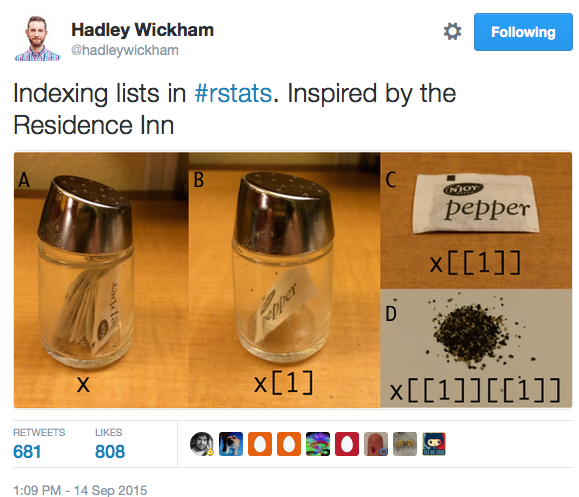
\includegraphics[width=0.5\textwidth,height=\textheight]{./figures/wickham_indexing_tweet.png}}

\begin{Shaded}
\begin{Highlighting}[]
\CommentTok{\# Numeric subsetting                                                          {-}{-}{-}{-}}
\CommentTok{\# {-} {-} {-} {-} {-} {-} {-} {-} {-} {-} {-} {-} {-} {-} {-} {-} {-} {-} {-} {-} {-} {-} {-} {-} {-} {-} {-} {-} {-} {-} {-} {-} {-} {-} {-} {-} {-} {-} {-} }

\CommentTok{\# Let\textquotesingle{}s use our vector of ego age values again.}
\NormalTok{age}
\end{Highlighting}
\end{Shaded}

\begin{verbatim}
##  [1] 29 55 54 59 52 62 30 42 44 52
\end{verbatim}

\begin{Shaded}
\begin{Highlighting}[]
\CommentTok{\# Index its 2nd element: The age of the 2nd respondent.}
\NormalTok{age[}\DecValTok{2}\NormalTok{]}
\end{Highlighting}
\end{Shaded}

\begin{verbatim}
## [1] 55
\end{verbatim}

\begin{Shaded}
\begin{Highlighting}[]
\CommentTok{\# Its 2nd, 4th and 5th elements.}
\NormalTok{age[}\FunctionTok{c}\NormalTok{(}\DecValTok{2}\NormalTok{,}\DecValTok{4}\NormalTok{,}\DecValTok{5}\NormalTok{)]}
\end{Highlighting}
\end{Shaded}

\begin{verbatim}
## [1] 55 59 52
\end{verbatim}

\begin{Shaded}
\begin{Highlighting}[]
\CommentTok{\# Fifth to seventh elements}
\NormalTok{age[}\DecValTok{5}\SpecialCharTok{:}\DecValTok{7}\NormalTok{]}
\end{Highlighting}
\end{Shaded}

\begin{verbatim}
## [1] 52 62 30
\end{verbatim}

\begin{Shaded}
\begin{Highlighting}[]
\CommentTok{\# Use indexing to assign (replace) an element.}
\NormalTok{age[}\DecValTok{2}\NormalTok{] }\OtherTok{\textless{}{-}} \DecValTok{45}

\CommentTok{\# The content of x has now changed.}
\NormalTok{age}
\end{Highlighting}
\end{Shaded}

\begin{verbatim}
##  [1] 29 45 54 59 52 62 30 42 44 52
\end{verbatim}

\begin{Shaded}
\begin{Highlighting}[]
\CommentTok{\# Let\textquotesingle{}s subset the adjacency matrix we created before.}
\NormalTok{adj}
\end{Highlighting}
\end{Shaded}

\begin{verbatim}
##      [,1] [,2] [,3]
## [1,]    0    1    1
## [2,]    1    0    1
## [3,]    0    0    0
\end{verbatim}

\begin{Shaded}
\begin{Highlighting}[]
\CommentTok{\# Its 2,3 cell: Edge from node 2 to node 3.}
\NormalTok{adj[}\DecValTok{2}\NormalTok{,}\DecValTok{3}\NormalTok{]}
\end{Highlighting}
\end{Shaded}

\begin{verbatim}
## [1] 1
\end{verbatim}

\begin{Shaded}
\begin{Highlighting}[]
\CommentTok{\# Its 2nd column: All edges to node 2.}
\NormalTok{adj[,}\DecValTok{2}\NormalTok{]}
\end{Highlighting}
\end{Shaded}

\begin{verbatim}
## [1] 1 0 0
\end{verbatim}

\begin{Shaded}
\begin{Highlighting}[]
\CommentTok{\# Its 2nd and 3rd row: All edges from nodes 2 and 3.}
\NormalTok{adj[}\DecValTok{2}\SpecialCharTok{:}\DecValTok{3}\NormalTok{,]}
\end{Highlighting}
\end{Shaded}

\begin{verbatim}
##      [,1] [,2] [,3]
## [1,]    1    0    1
## [2,]    0    0    0
\end{verbatim}

\begin{Shaded}
\begin{Highlighting}[]
\CommentTok{\# Logical subsetting                                                          {-}{-}{-}{-}}
\CommentTok{\# {-} {-} {-} {-} {-} {-} {-} {-} {-} {-} {-} {-} {-} {-} {-} {-} {-} {-} {-} {-} {-} {-} {-} {-} {-} {-} {-} {-} {-} {-} {-} {-} {-} {-} {-} {-} {-} {-} {-} }

\CommentTok{\# Which values of "age" are between 40 and 60?}

\CommentTok{\# Let\textquotesingle{}s create a logical index that flags these values.}
\NormalTok{(ind }\OtherTok{\textless{}{-}}\NormalTok{ age }\SpecialCharTok{\textgreater{}} \DecValTok{40} \SpecialCharTok{\&}\NormalTok{ age }\SpecialCharTok{\textless{}} \DecValTok{60}\NormalTok{)}
\end{Highlighting}
\end{Shaded}

\begin{verbatim}
##  [1] FALSE  TRUE  TRUE  TRUE  TRUE FALSE FALSE  TRUE  TRUE  TRUE
\end{verbatim}

\begin{Shaded}
\begin{Highlighting}[]
\CommentTok{\# Use this index to extract these values from vector "age" via logical subsetting.}
\NormalTok{age[ind]}
\end{Highlighting}
\end{Shaded}

\begin{verbatim}
## [1] 45 54 59 52 42 44 52
\end{verbatim}

\begin{Shaded}
\begin{Highlighting}[]
\CommentTok{\# We could also have typed directly:}
\NormalTok{age[age }\SpecialCharTok{\textgreater{}} \DecValTok{40} \SpecialCharTok{\&}\NormalTok{ age }\SpecialCharTok{\textless{}} \DecValTok{60}\NormalTok{]}
\end{Highlighting}
\end{Shaded}

\begin{verbatim}
## [1] 45 54 59 52 42 44 52
\end{verbatim}

\begin{Shaded}
\begin{Highlighting}[]
\CommentTok{\# Subsetting data frames                                                     {-}{-}{-}{-} }
\CommentTok{\# {-} {-} {-} {-} {-} {-} {-} {-} {-} {-} {-} {-} {-} {-} {-} {-} {-} {-} {-} {-} {-} {-} {-} {-} {-} {-} {-} {-} {-} {-} {-} {-} {-} {-} {-} {-} {-} {-} {-} }

\CommentTok{\# We\textquotesingle{}ll use our data frame (just its first 20 rows).}
\NormalTok{data}\FloatTok{.20} \OtherTok{\textless{}{-}} \FunctionTok{slice}\NormalTok{(data, }\DecValTok{1}\SpecialCharTok{:}\DecValTok{20}\NormalTok{)}

\CommentTok{\# Numeric subsetting works on data frames too: it allows you to index variables.}

\CommentTok{\# The 3rd variable.}
\NormalTok{data}\FloatTok{.20}\NormalTok{[}\DecValTok{3}\NormalTok{]}
\end{Highlighting}
\end{Shaded}

\begin{verbatim}
## # A tibble: 20 x 1
##    `4. Sei nato/a in Italia?`
##    <chr>                     
##  1 Sì                        
##  2 No                        
##  3 Sì                        
##  4 Sì                        
##  5 Sì                        
##  6 Sì                        
##  7 Sì                        
##  8 Sì                        
##  9 Sì                        
## 10 Sì                        
## 11 Sì                        
## 12 Sì                        
## 13 Sì                        
## 14 Sì                        
## 15 Sì                        
## 16 Sì                        
## 17 Sì                        
## 18 Sì                        
## 19 Sì                        
## 20 Sì
\end{verbatim}

\begin{Shaded}
\begin{Highlighting}[]
\CommentTok{\# Note the difference with the double square bracket.}
\NormalTok{data}\FloatTok{.20}\NormalTok{[[}\DecValTok{3}\NormalTok{]]}
\end{Highlighting}
\end{Shaded}

\begin{verbatim}
##  [1] "Sì" "No" "Sì" "Sì" "Sì" "Sì" "Sì" "Sì" "Sì" "Sì" "Sì" "Sì" "Sì" "Sì" "Sì"
## [16] "Sì" "Sì" "Sì" "Sì" "Sì"
\end{verbatim}

\begin{Shaded}
\begin{Highlighting}[]
\CommentTok{\# What do you think is the difference?}
\FunctionTok{class}\NormalTok{(data}\FloatTok{.20}\NormalTok{[}\DecValTok{3}\NormalTok{])}
\end{Highlighting}
\end{Shaded}

\begin{verbatim}
## [1] "tbl_df"     "tbl"        "data.frame"
\end{verbatim}

\begin{Shaded}
\begin{Highlighting}[]
\FunctionTok{class}\NormalTok{(data}\FloatTok{.20}\NormalTok{[[}\DecValTok{3}\NormalTok{]])}
\end{Highlighting}
\end{Shaded}

\begin{verbatim}
## [1] "character"
\end{verbatim}

\begin{Shaded}
\begin{Highlighting}[]
\CommentTok{\# The [[ ]] notation extracts the actual column as a vector, while [ ] keeps}
\CommentTok{\# the data frame class.}

\CommentTok{\# We can also subset data frames as matrices.}
\CommentTok{\# The second and third columns.}
\NormalTok{data}\FloatTok{.20}\NormalTok{[,}\DecValTok{2}\SpecialCharTok{:}\DecValTok{3}\NormalTok{]}
\end{Highlighting}
\end{Shaded}

\begin{verbatim}
## # A tibble: 20 x 2
##    `2. Il tuo genere è...`                                4. Sei nato/a in Ita~1
##    <chr>                                                  <chr>                 
##  1 Uomo                                                   Sì                    
##  2 Donna                                                  No                    
##  3 Uomo                                                   Sì                    
##  4 Uomo                                                   Sì                    
##  5 Uomo                                                   Sì                    
##  6 Preferisco non rispondere                              Sì                    
##  7 Donna                                                  Sì                    
##  8 Uomo                                                   Sì                    
##  9 Donna                                                  Sì                    
## 10 Uomo                                                   Sì                    
## 11 Uomo                                                   Sì                    
## 12 Donna                                                  Sì                    
## 13 Donna                                                  Sì                    
## 14 Altra identità di genere (transgender, non binario, e~ Sì                    
## 15 Uomo                                                   Sì                    
## 16 Donna                                                  Sì                    
## 17 Donna                                                  Sì                    
## 18 Uomo                                                   Sì                    
## 19 Uomo                                                   Sì                    
## 20 Uomo                                                   Sì                    
## # i abbreviated name: 1: `4. Sei nato/a in Italia?`
\end{verbatim}

\begin{Shaded}
\begin{Highlighting}[]
\CommentTok{\# Lines 1 to 3}
\NormalTok{data}\FloatTok{.20}\NormalTok{[}\DecValTok{1}\SpecialCharTok{:}\DecValTok{3}\NormalTok{,]}
\end{Highlighting}
\end{Shaded}

\begin{verbatim}
## # A tibble: 3 x 7
##   `1. Il tuo anno di nascita è...` 2. Il tuo genere è..~1 4. Sei nato/a in Ita~2
##                              <dbl> <chr>                  <chr>                 
## 1                             1994 Uomo                   Sì                    
## 2                             1968 Donna                  No                    
## 3                             1969 Uomo                   Sì                    
## # i abbreviated names: 1: `2. Il tuo genere è...`,
## #   2: `4. Sei nato/a in Italia?`
## # i 4 more variables:
## #   `11. Il tuo ultimo titolo di studi conseguito è...` <chr>, company <chr>,
## #   work.exp.y <dbl>, driver.sum <dbl>
\end{verbatim}

\begin{Shaded}
\begin{Highlighting}[]
\CommentTok{\# We can use name indexing with data frames, selecting variables by name}
\NormalTok{data}\FloatTok{.20}\NormalTok{[}\StringTok{"company"}\NormalTok{]}
\end{Highlighting}
\end{Shaded}

\begin{verbatim}
## # A tibble: 20 x 1
##    company             
##    <chr>               
##  1 My Vegetarian Dinner
##  2 Urban Gallery       
##  3 Office Tile         
##  4 Raven               
##  5 Fix Guru            
##  6 Office Brush        
##  7 House Brush         
##  8 Satan's Sister      
##  9 FruityFlix          
## 10 Coal Kings          
## 11 Coal Kings          
## 12 Coal Kings          
## 13 Coal Kings          
## 14 Beep Sports         
## 15 The Auto DNA        
## 16 Office Tile         
## 17 Coal Kings          
## 18 Wood Works          
## 19 Bloom Marketing     
## 20 Coal Kings
\end{verbatim}

\begin{Shaded}
\begin{Highlighting}[]
\NormalTok{data}\FloatTok{.20}\NormalTok{[[}\StringTok{"company"}\NormalTok{]]}
\end{Highlighting}
\end{Shaded}

\begin{verbatim}
##  [1] "My Vegetarian Dinner" "Urban Gallery"        "Office Tile"         
##  [4] "Raven"                "Fix Guru"             "Office Brush"        
##  [7] "House Brush"          "Satan's Sister"       "FruityFlix"          
## [10] "Coal Kings"           "Coal Kings"           "Coal Kings"          
## [13] "Coal Kings"           "Beep Sports"          "The Auto DNA"        
## [16] "Office Tile"          "Coal Kings"           "Wood Works"          
## [19] "Bloom Marketing"      "Coal Kings"
\end{verbatim}

\begin{Shaded}
\begin{Highlighting}[]
\CommentTok{\# The $ notation is very common and concise. It\textquotesingle{}s equivalent to the [[ notation.}
\NormalTok{data}\FloatTok{.20}\SpecialCharTok{$}\NormalTok{company}
\end{Highlighting}
\end{Shaded}

\begin{verbatim}
##  [1] "My Vegetarian Dinner" "Urban Gallery"        "Office Tile"         
##  [4] "Raven"                "Fix Guru"             "Office Brush"        
##  [7] "House Brush"          "Satan's Sister"       "FruityFlix"          
## [10] "Coal Kings"           "Coal Kings"           "Coal Kings"          
## [13] "Coal Kings"           "Beep Sports"          "The Auto DNA"        
## [16] "Office Tile"          "Coal Kings"           "Wood Works"          
## [19] "Bloom Marketing"      "Coal Kings"
\end{verbatim}

\begin{Shaded}
\begin{Highlighting}[]
\CommentTok{\# This is the same as data.20[[3]] or data.20[["ego.age"]]}
\FunctionTok{identical}\NormalTok{(data}\FloatTok{.20}\NormalTok{[[}\DecValTok{5}\NormalTok{]], data}\FloatTok{.20}\SpecialCharTok{$}\NormalTok{company)}
\end{Highlighting}
\end{Shaded}

\begin{verbatim}
## [1] TRUE
\end{verbatim}

\begin{Shaded}
\begin{Highlighting}[]
\CommentTok{\# With tidyverse, this type of subsetting syntax is replaced by new "verbs" }
\CommentTok{\# (see next chapter):}
\CommentTok{\# * Index data frame rows: filter() instead of []}
\CommentTok{\# * Index data frame columns: select() instead of []}
\CommentTok{\# * Extract data frame variable as a vector: pull() instead of [[]] or $}


\CommentTok{\# ***** EXERCISES }
\CommentTok{\#}
\CommentTok{\# Create the fictitious variable var \textless{}{-} c(1:30, rep(NA, 3), 34:50). Use is.na()}
\CommentTok{\# to index all the NA values in the variable. Then use is.na() to index all}
\CommentTok{\# values that are *not* NA. Hint: Remember the operator used to negate a logical}
\CommentTok{\# vector. Finally, use this indexing to remove all NA values from var.}
\CommentTok{\#}
\CommentTok{\# *****}
\end{Highlighting}
\end{Shaded}

\hypertarget{pipes-and-the-operator}{%
\section{\texorpdfstring{Pipes and the \texttt{\textbar{}\textgreater{}} operator}{Pipes and the \textbar\textgreater{} operator}}\label{pipes-and-the-operator}}

\begin{itemize}
\tightlist
\item
  The original pipe operator, \texttt{\%\textgreater{}\%}, was introduced by the \texttt{magrittr} package in 2014. It quickly gained popularity in the R community and was adopted by \texttt{tidyverse} (and other packages). In 2021, R incorporated the pipe idea with a new, similar (but not identical) operator: \texttt{\textbar{}\textgreater{}}. See \href{https://www.tidyverse.org/blog/2023/04/base-vs-magrittr-pipe/}{this page} for an overview of the differences between \texttt{\textbar{}\textgreater{}} and \texttt{\%\textgreater{}\%}.
\item
  The idea behind pipes is in essence very simple:

  \begin{itemize}
  \tightlist
  \item
    \texttt{f(g(x))} becomes \texttt{x\ \textbar{}\textgreater{}\ g()\ \textbar{}\textgreater{}\ f()}.
  \item
    For example: \texttt{mean(table(x))} becomes \texttt{x\ \textbar{}\textgreater{}\ table()\ \textbar{}\textgreater{}\ mean()}.
  \end{itemize}
\item
  So \texttt{\textbar{}\textgreater{}} pipes the output of the previous function (e.g., \texttt{table()}) into the input of the following function (e.g., \texttt{mean()}). This turns inside-to-outside code into left-to-right code. Because left to right is the direction most of us are used to read in (at least in English and other Western languages), pipes make R code easier to read and follow.
\item
  You may also see pipes concatenating multiple lines of code. That's possible and a common coding style. Instead of
\end{itemize}

\begin{verbatim}
x |> table() |> mean()
\end{verbatim}

you can write

\begin{verbatim}
x |>
  table() |>
  mean()
\end{verbatim}

Let's see how this works with some of our data objects.

\begin{Shaded}
\begin{Highlighting}[]
\CommentTok{\# Respondent gender variable }
\NormalTok{gender }\OtherTok{\textless{}{-}}\NormalTok{ data[[}\DecValTok{2}\NormalTok{]]}

\CommentTok{\# First 10 values}
\NormalTok{gender[}\DecValTok{1}\SpecialCharTok{:}\DecValTok{10}\NormalTok{]}
\end{Highlighting}
\end{Shaded}

\begin{verbatim}
##  [1] "Uomo"                      "Donna"                    
##  [3] "Uomo"                      "Uomo"                     
##  [5] "Uomo"                      "Preferisco non rispondere"
##  [7] "Donna"                     "Uomo"                     
##  [9] "Donna"                     "Uomo"
\end{verbatim}

\begin{Shaded}
\begin{Highlighting}[]
\CommentTok{\# Frequency of gender categories in the data}
\FunctionTok{table}\NormalTok{(gender)}
\end{Highlighting}
\end{Shaded}

\begin{verbatim}
## gender
## Altra identità di genere (transgender, non binario, ecc.) 
##                                                         3 
##                                                     Donna 
##                                                       522 
##                                 Preferisco non rispondere 
##                                                         8 
##                                                      Uomo 
##                                                       467
\end{verbatim}

\begin{Shaded}
\begin{Highlighting}[]
\CommentTok{\# Average frequency}
\FunctionTok{mean}\NormalTok{(}\FunctionTok{table}\NormalTok{(gender))}
\end{Highlighting}
\end{Shaded}

\begin{verbatim}
## [1] 250
\end{verbatim}

\begin{Shaded}
\begin{Highlighting}[]
\CommentTok{\# Let\textquotesingle{}s re{-}write this with the pipe operator}
\NormalTok{gender }\SpecialCharTok{|\textgreater{}} 
  \FunctionTok{table}\NormalTok{() }\SpecialCharTok{|\textgreater{}} 
  \FunctionTok{mean}\NormalTok{()}
\end{Highlighting}
\end{Shaded}

\begin{verbatim}
## [1] 250
\end{verbatim}

\hypertarget{functions}{%
\section{Writing your own R functions}\label{functions}}

\begin{itemize}
\tightlist
\item
  One of the most powerful tools in R is the ability to \textbf{write your own functions}.
\item
  A function is a \textbf{piece of code} that operates on one or multiple \textbf{arguments} (the \emph{input}), and returns an \emph{output} (the function \textbf{value} in R terminology). Everything that happens in R is done by a function.
\item
  Many R functions have \textbf{default values} for their arguments: if you don't specify the argument's value, the function will use the default.
\item
  Once you write a function and define its arguments, you can run that function on any argument values you want --- provided that the function code actually works on those argument values.
\item
  R functions, combined with \href{https://adv-r.hadley.nz/functionals.html}{functionals} and summarization methods, are the best way to run exactly the same code on many different objects. Functions are \textbf{crucial for code reproducibility} in R. If you write functions, you won't need to re-write (copy and paste) the same code over and over again --- you just write it once in the function, then run the function any time and on any arguments you need. This yields clearer, shorter, more readable code with less errors.
\item
  New functions are also commonly used to \textbf{redefine existing functions} by pre-setting the value of specific arguments. For example, if you want all your plots to have \texttt{red} as color, you can take R's existing plotting function \texttt{plot()}, and wrap it in a new function that always executes \texttt{plot()} with the argument \texttt{col="red"}. Your function would be something like \texttt{my.plot\ \textless{}-\ function(...)\ \{plot(...,\ col="red")\}}.
\item
  \textbf{Tips and tricks} with functions:

  \begin{itemize}
  \tightlist
  \item
    \texttt{stopifnot()} is useful to check that function arguments are of the type that was intended by the function author. It stops the function if a certain condition is not met by a function argument (e.g., argument is \emph{not} a \texttt{numeric} object, if the function was written for \texttt{numeric} objects).
  \item
    \texttt{return()} allows you to explicitly set the output that the function will return (clearer code). It is also used to stop function execution earlier under certain conditions. Note: If you don't use \texttt{return()}, the function value (output) is the last object that is printed at the end of the function code.
  \item
    \texttt{if} is a flow control tool that is frequently used within functions: it specifies what the function should do \texttt{if} a certain condition is met at one point.
  \item
    First think particular, then generalize. When you want to write a function, it's a good idea to first try the code on a ``real'', specific existing object in your workspace. If the code does what you want on that object, you can then wrap it into a general function to be run on any similar object (see examples in the code below).
  \end{itemize}
\end{itemize}

\begin{Shaded}
\begin{Highlighting}[]
\CommentTok{\# Any piece of code you can write and run in R, you can also put in a function.}

\CommentTok{\# Let\textquotesingle{}s write a trivial function that takes its argument and multiplies it by 2.}
\NormalTok{times2 }\OtherTok{\textless{}{-}} \ControlFlowTok{function}\NormalTok{(x) \{}
\NormalTok{  x}\SpecialCharTok{*}\DecValTok{2}
\NormalTok{\}}

\CommentTok{\# Now we can run the function on any argument.}
\FunctionTok{times2}\NormalTok{(}\AttributeTok{x=} \DecValTok{3}\NormalTok{)}
\end{Highlighting}
\end{Shaded}

\begin{verbatim}
## [1] 6
\end{verbatim}

\begin{Shaded}
\begin{Highlighting}[]
\FunctionTok{times2}\NormalTok{(}\AttributeTok{x=} \DecValTok{10}\NormalTok{)}
\end{Highlighting}
\end{Shaded}

\begin{verbatim}
## [1] 20
\end{verbatim}

\begin{Shaded}
\begin{Highlighting}[]
\FunctionTok{times2}\NormalTok{(}\DecValTok{50}\NormalTok{)}
\end{Highlighting}
\end{Shaded}

\begin{verbatim}
## [1] 100
\end{verbatim}

\begin{Shaded}
\begin{Highlighting}[]
\CommentTok{\# A function that takes its argument and prints a sentence with it:}
\NormalTok{myoutput }\OtherTok{\textless{}{-}} \ControlFlowTok{function}\NormalTok{(word) \{}
  \FunctionTok{print}\NormalTok{(}\FunctionTok{paste}\NormalTok{(}\StringTok{"My output is"}\NormalTok{, word))}
\NormalTok{\}}

\CommentTok{\# Let\textquotesingle{}s run the function.}
\FunctionTok{myoutput}\NormalTok{(}\StringTok{"cat"}\NormalTok{)}
\end{Highlighting}
\end{Shaded}

\begin{verbatim}
## [1] "My output is cat"
\end{verbatim}

\begin{Shaded}
\begin{Highlighting}[]
\FunctionTok{myoutput}\NormalTok{(}\AttributeTok{word=} \StringTok{"table"}\NormalTok{)}
\end{Highlighting}
\end{Shaded}

\begin{verbatim}
## [1] "My output is table"
\end{verbatim}

\begin{Shaded}
\begin{Highlighting}[]
\FunctionTok{myoutput}\NormalTok{(}\StringTok{"any word here"}\NormalTok{)}
\end{Highlighting}
\end{Shaded}

\begin{verbatim}
## [1] "My output is any word here"
\end{verbatim}

\begin{Shaded}
\begin{Highlighting}[]
\CommentTok{\# Not a particularly useful function...}

\CommentTok{\# Note that the function output is the last object that is printed at the end}
\CommentTok{\# of the function code.}
\NormalTok{times2 }\OtherTok{\textless{}{-}} \ControlFlowTok{function}\NormalTok{(x) \{}
\NormalTok{  y }\OtherTok{\textless{}{-}}\NormalTok{ x}\SpecialCharTok{*}\DecValTok{2}
\NormalTok{  y}
\NormalTok{\}}
\FunctionTok{times2}\NormalTok{(}\AttributeTok{x=}\DecValTok{4}\NormalTok{)}
\end{Highlighting}
\end{Shaded}

\begin{verbatim}
## [1] 8
\end{verbatim}

\begin{Shaded}
\begin{Highlighting}[]
\CommentTok{\# If nothing is printed, then the function returns nothing.}
\NormalTok{times2 }\OtherTok{\textless{}{-}} \ControlFlowTok{function}\NormalTok{(x) \{}
\NormalTok{  y }\OtherTok{\textless{}{-}}\NormalTok{ x}\SpecialCharTok{*}\DecValTok{2}
\NormalTok{\}}
\FunctionTok{times2}\NormalTok{(}\AttributeTok{x=}\DecValTok{4}\NormalTok{)}

\CommentTok{\# A function will return an error if it\textquotesingle{}s executed on arguments that are not}
\CommentTok{\# suitable for the code inside the function. E.g., R can\textquotesingle{}t multiply "a" by 2...}
\NormalTok{times2 }\OtherTok{\textless{}{-}} \ControlFlowTok{function}\NormalTok{(x) \{}
\NormalTok{  x}\SpecialCharTok{*}\DecValTok{2}
\NormalTok{\}}
\FunctionTok{times2}\NormalTok{(}\AttributeTok{x=} \StringTok{"a"}\NormalTok{)}
\end{Highlighting}
\end{Shaded}

\begin{verbatim}
## Error in x * 2: non-numeric argument to binary operator
\end{verbatim}

\begin{Shaded}
\begin{Highlighting}[]
\CommentTok{\# Let\textquotesingle{}s then specify that the function\textquotesingle{}s argument must be numeric.}
\NormalTok{times2 }\OtherTok{\textless{}{-}} \ControlFlowTok{function}\NormalTok{(x) \{}
  \FunctionTok{stopifnot}\NormalTok{(}\FunctionTok{is.numeric}\NormalTok{(x))  }
\NormalTok{  x}\SpecialCharTok{*}\DecValTok{2}
\NormalTok{\}}

\CommentTok{\# Let\textquotesingle{}s try it now.}
\FunctionTok{times2}\NormalTok{(}\AttributeTok{x=} \StringTok{"a"}\NormalTok{)}
\end{Highlighting}
\end{Shaded}

\begin{verbatim}
## Error in times2(x = "a"): is.numeric(x) is not TRUE
\end{verbatim}

\begin{Shaded}
\begin{Highlighting}[]
\CommentTok{\# This still throws and error, but it makes the error clearer to the user and }
\CommentTok{\# it immediately indicates where the problem is.}

\CommentTok{\# Using if, we can also re{-}write the function so that it returns NA with a}
\CommentTok{\# warning if its argument is not numeric {-}{-} instead of just stopping with an}
\CommentTok{\# error.}
\NormalTok{times2 }\OtherTok{\textless{}{-}} \ControlFlowTok{function}\NormalTok{(x) \{}
  \CommentTok{\# If x is not numeric}
  \ControlFlowTok{if}\NormalTok{(}\SpecialCharTok{!}\FunctionTok{is.numeric}\NormalTok{(x)) \{}
    \CommentTok{\# Give the warning}
    \FunctionTok{warning}\NormalTok{(}\StringTok{"Your argument is not numeric!"}\NormalTok{, }\AttributeTok{call. =} \ConstantTok{FALSE}\NormalTok{)}
    \CommentTok{\# Return missing value}
    \FunctionTok{return}\NormalTok{(}\ConstantTok{NA}\NormalTok{)}
    \CommentTok{\# Otherwise, return x*2}
\NormalTok{  \} }\ControlFlowTok{else}\NormalTok{ \{}
    \FunctionTok{return}\NormalTok{(x}\SpecialCharTok{*}\DecValTok{2}\NormalTok{)}
\NormalTok{  \}}
\NormalTok{\}}

\CommentTok{\# Try the function}
\FunctionTok{times2}\NormalTok{(}\DecValTok{2}\NormalTok{)}
\end{Highlighting}
\end{Shaded}

\begin{verbatim}
## [1] 4
\end{verbatim}

\begin{Shaded}
\begin{Highlighting}[]
\FunctionTok{times2}\NormalTok{(}\StringTok{"a"}\NormalTok{)}
\end{Highlighting}
\end{Shaded}

\begin{verbatim}
## Warning: Your argument is not numeric!
\end{verbatim}

\begin{verbatim}
## [1] NA
\end{verbatim}

\hypertarget{types-and-classes-of-objects}{%
\section{Types and classes of objects}\label{types-and-classes-of-objects}}

This is a quick summary of the basics about \textbf{types} and \textbf{classes} of objects in R.

\begin{itemize}
\item
  Three functions are used to know what kind of object you are dealing with in R: \texttt{class()}, \texttt{mode()}, and \texttt{typeof()}.
\item
  For most purposes, you only need to know what the \textbf{class} of an object is. This is returned by \texttt{class()}. The class of an object determines what R functions you can or cannot run on that object, and how functions will behave when you run them on the object. In particular, if the function has a \texttt{method} for a specific class \emph{A} of objects, it will use that method whenever an object of class \emph{A} is given as its argument.
\item
  \texttt{typeof()} and \texttt{mode()} return the \textbf{type} and \textbf{mode} of an object, respectively. Although they refer to slightly different classifications of objects, type and mode give essentially the same kind of information --- the type of data structure in which the object is stored, also called the R ``internal type'' or ``storage mode''. For example, an object can be internally stored in R as double-precision numbers, integer numbers, or character strings.

  \begin{itemize}
  \tightlist
  \item
    You should prefer \texttt{typeof()} over \texttt{mode()}. \texttt{mode()} refers to the old S classification of types and is mostly used for S compatibility.
  \end{itemize}
\item
  While most times all you need to know is the \texttt{class} of an object, there are a few cases in which knowing the \texttt{type} is useful too. For example, you may want to know the \texttt{type} of a matrix object (whose \texttt{class} is always \texttt{matrix}) to check if the values in the matrix are being stored as numbers or character strings (that will affect the result of some functions).
\item
  Main classes/types of objects

  \begin{itemize}
  \tightlist
  \item
    \texttt{numeric}: Numerical data (integer, real or complex numbers).
  \item
    \texttt{logical}: \texttt{TRUE/FALSE} data.
  \item
    \texttt{character}: String data.
  \item
    \texttt{factor}: Categorical data, that is, integer numbers with string labels attached. May be \emph{unordered} factors (nominal data) or \emph{ordered} factors (ordinal data).
  \end{itemize}
\item
  Special and complex classes/types

  \begin{itemize}
  \tightlist
  \item
    \texttt{list}: A collection of elements of any type, including numeric, character, logical.
  \item
    \texttt{data.frame}: A dataset. In R, a data frame is a special kind of list (its type is \texttt{list} but its class is \texttt{data.frame}), where each variable (column) is a list element (see Section \ref{dataframes})
  \item
    \texttt{matrix}: Matrix values can be numeric, character, logical etc. So an object can have \texttt{matrix} as class and \texttt{numeric}, \texttt{character} or \texttt{logical} as type. While data frames can contain variables of different type (e.g.~a character variable and a numeric variable), matrices can only contain values of \emph{one} type.
  \item
    Functions (more on this in Section \ref{functions}).
  \item
    Expressions.
  \item
    Formulas.
  \item
    Other objects: Statistical results (e.g.~linear model estimates), dendrograms, graphics objects, etc.
  \end{itemize}
\item
  Relevant functions

  \begin{itemize}
  \tightlist
  \item
    \texttt{class()}, \texttt{typeof()} and \texttt{mode()}, as discussed above.
  \item
    \texttt{is.}\emph{type} functions verify that an object is in a specific type or class: e.g.~\texttt{is.numeric(x)}, \texttt{is.character(x)} (they return \texttt{TRUE} or \texttt{FALSE}).
  \item
    \texttt{as.}\emph{type} functions convert objects between types or classes: e.g.~\texttt{as.numeric()}, \texttt{as.character()}. If the conversion is impossible, the result is \texttt{NA}: e.g.~\texttt{as.numeric("abc")} returns \texttt{NA}.
  \end{itemize}
\end{itemize}

\begin{Shaded}
\begin{Highlighting}[]
\CommentTok{\# A numeric vector of integers.}
\NormalTok{n }\OtherTok{\textless{}{-}} \DecValTok{1}\SpecialCharTok{:}\DecValTok{100}

\CommentTok{\# Let\textquotesingle{}s check the class and type.}
\FunctionTok{class}\NormalTok{(n)}
\end{Highlighting}
\end{Shaded}

\begin{verbatim}
## [1] "integer"
\end{verbatim}

\begin{Shaded}
\begin{Highlighting}[]
\FunctionTok{typeof}\NormalTok{(n)}
\end{Highlighting}
\end{Shaded}

\begin{verbatim}
## [1] "integer"
\end{verbatim}

\begin{Shaded}
\begin{Highlighting}[]
\CommentTok{\# A character object.}
\NormalTok{(char }\OtherTok{\textless{}{-}} \FunctionTok{c}\NormalTok{(}\StringTok{"a"}\NormalTok{, }\StringTok{"b"}\NormalTok{, }\StringTok{"c"}\NormalTok{, }\StringTok{"d"}\NormalTok{, }\StringTok{"e"}\NormalTok{, }\StringTok{"f"}\NormalTok{))}
\end{Highlighting}
\end{Shaded}

\begin{verbatim}
## [1] "a" "b" "c" "d" "e" "f"
\end{verbatim}

\begin{Shaded}
\begin{Highlighting}[]
\CommentTok{\# Class and type.}
\FunctionTok{class}\NormalTok{(char)}
\end{Highlighting}
\end{Shaded}

\begin{verbatim}
## [1] "character"
\end{verbatim}

\begin{Shaded}
\begin{Highlighting}[]
\FunctionTok{typeof}\NormalTok{(char)}
\end{Highlighting}
\end{Shaded}

\begin{verbatim}
## [1] "character"
\end{verbatim}

\begin{Shaded}
\begin{Highlighting}[]
\CommentTok{\# Let\textquotesingle{}s put n in a matrix.}
\NormalTok{(M }\OtherTok{\textless{}{-}} \FunctionTok{matrix}\NormalTok{(n, }\AttributeTok{nrow=}\DecValTok{10}\NormalTok{, }\AttributeTok{ncol=}\DecValTok{10}\NormalTok{))}
\end{Highlighting}
\end{Shaded}

\begin{verbatim}
##       [,1] [,2] [,3] [,4] [,5] [,6] [,7] [,8] [,9] [,10]
##  [1,]    1   11   21   31   41   51   61   71   81    91
##  [2,]    2   12   22   32   42   52   62   72   82    92
##  [3,]    3   13   23   33   43   53   63   73   83    93
##  [4,]    4   14   24   34   44   54   64   74   84    94
##  [5,]    5   15   25   35   45   55   65   75   85    95
##  [6,]    6   16   26   36   46   56   66   76   86    96
##  [7,]    7   17   27   37   47   57   67   77   87    97
##  [8,]    8   18   28   38   48   58   68   78   88    98
##  [9,]    9   19   29   39   49   59   69   79   89    99
## [10,]   10   20   30   40   50   60   70   80   90   100
\end{verbatim}

\begin{Shaded}
\begin{Highlighting}[]
\CommentTok{\# Class/type of this object.}
\FunctionTok{class}\NormalTok{(M)}
\end{Highlighting}
\end{Shaded}

\begin{verbatim}
## [1] "matrix" "array"
\end{verbatim}

\begin{Shaded}
\begin{Highlighting}[]
\CommentTok{\# Type and mode tell us that this is an *integer* matrix.}
\FunctionTok{typeof}\NormalTok{(M)}
\end{Highlighting}
\end{Shaded}

\begin{verbatim}
## [1] "integer"
\end{verbatim}

\begin{Shaded}
\begin{Highlighting}[]
\CommentTok{\# There are character and logical matrices too.}
\NormalTok{char}
\end{Highlighting}
\end{Shaded}

\begin{verbatim}
## [1] "a" "b" "c" "d" "e" "f"
\end{verbatim}

\begin{Shaded}
\begin{Highlighting}[]
\NormalTok{(C }\OtherTok{\textless{}{-}} \FunctionTok{matrix}\NormalTok{(char, }\AttributeTok{nrow=}\DecValTok{3}\NormalTok{, }\AttributeTok{ncol=} \DecValTok{2}\NormalTok{))}
\end{Highlighting}
\end{Shaded}

\begin{verbatim}
##      [,1] [,2]
## [1,] "a"  "d" 
## [2,] "b"  "e" 
## [3,] "c"  "f"
\end{verbatim}

\begin{Shaded}
\begin{Highlighting}[]
\CommentTok{\# Class and type.}
\FunctionTok{class}\NormalTok{(C)}
\end{Highlighting}
\end{Shaded}

\begin{verbatim}
## [1] "matrix" "array"
\end{verbatim}

\begin{Shaded}
\begin{Highlighting}[]
\FunctionTok{typeof}\NormalTok{(C)}
\end{Highlighting}
\end{Shaded}

\begin{verbatim}
## [1] "character"
\end{verbatim}

\begin{Shaded}
\begin{Highlighting}[]
\CommentTok{\# Notice that a matrix can contain numbers but still be stored as character.}
\NormalTok{(M }\OtherTok{\textless{}{-}} \FunctionTok{matrix}\NormalTok{(}\FunctionTok{c}\NormalTok{(}\StringTok{"1"}\NormalTok{, }\StringTok{"2"}\NormalTok{, }\StringTok{"3"}\NormalTok{, }\StringTok{"4"}\NormalTok{), }\AttributeTok{nrow=}\DecValTok{2}\NormalTok{, }\AttributeTok{ncol=}\DecValTok{2}\NormalTok{))}
\end{Highlighting}
\end{Shaded}

\begin{verbatim}
##      [,1] [,2]
## [1,] "1"  "3" 
## [2,] "2"  "4"
\end{verbatim}

\begin{Shaded}
\begin{Highlighting}[]
\FunctionTok{class}\NormalTok{(M)}
\end{Highlighting}
\end{Shaded}

\begin{verbatim}
## [1] "matrix" "array"
\end{verbatim}

\begin{Shaded}
\begin{Highlighting}[]
\FunctionTok{typeof}\NormalTok{(M)}
\end{Highlighting}
\end{Shaded}

\begin{verbatim}
## [1] "character"
\end{verbatim}

\begin{Shaded}
\begin{Highlighting}[]
\CommentTok{\# Let\textquotesingle{}s convert "char" to factor.}
\NormalTok{char}
\end{Highlighting}
\end{Shaded}

\begin{verbatim}
## [1] "a" "b" "c" "d" "e" "f"
\end{verbatim}

\begin{Shaded}
\begin{Highlighting}[]
\NormalTok{(char }\OtherTok{\textless{}{-}} \FunctionTok{as.factor}\NormalTok{(char))}
\end{Highlighting}
\end{Shaded}

\begin{verbatim}
## [1] a b c d e f
## Levels: a b c d e f
\end{verbatim}

\begin{Shaded}
\begin{Highlighting}[]
\CommentTok{\# This means that now char is not just a collection of strings, it is a}
\CommentTok{\# categorical variable in R\textquotesingle{}s mind: it is a collection of numbers with character}
\CommentTok{\# labels attached.}

\CommentTok{\# Compare the different behavior of as.numeric(): char as character...}
\NormalTok{(char }\OtherTok{\textless{}{-}} \FunctionTok{c}\NormalTok{(}\StringTok{"a"}\NormalTok{, }\StringTok{"b"}\NormalTok{, }\StringTok{"c"}\NormalTok{, }\StringTok{"d"}\NormalTok{, }\StringTok{"e"}\NormalTok{, }\StringTok{"f"}\NormalTok{))}
\end{Highlighting}
\end{Shaded}

\begin{verbatim}
## [1] "a" "b" "c" "d" "e" "f"
\end{verbatim}

\begin{Shaded}
\begin{Highlighting}[]
\CommentTok{\# Convert to numeric}
\FunctionTok{as.numeric}\NormalTok{(char)}
\end{Highlighting}
\end{Shaded}

\begin{verbatim}
## Warning: NAs introduced by coercion
\end{verbatim}

\begin{verbatim}
## [1] NA NA NA NA NA NA
\end{verbatim}

\begin{Shaded}
\begin{Highlighting}[]
\CommentTok{\# ...versus char as factor.}
\NormalTok{char }\OtherTok{\textless{}{-}} \FunctionTok{c}\NormalTok{(}\StringTok{"a"}\NormalTok{, }\StringTok{"b"}\NormalTok{, }\StringTok{"c"}\NormalTok{, }\StringTok{"d"}\NormalTok{, }\StringTok{"e"}\NormalTok{, }\StringTok{"f"}\NormalTok{)}
\NormalTok{(char }\OtherTok{\textless{}{-}} \FunctionTok{as.factor}\NormalTok{(char))}
\end{Highlighting}
\end{Shaded}

\begin{verbatim}
## [1] a b c d e f
## Levels: a b c d e f
\end{verbatim}

\begin{Shaded}
\begin{Highlighting}[]
\FunctionTok{as.numeric}\NormalTok{(char)}
\end{Highlighting}
\end{Shaded}

\begin{verbatim}
## [1] 1 2 3 4 5 6
\end{verbatim}

\begin{Shaded}
\begin{Highlighting}[]
\CommentTok{\# char is a different object in R\textquotesingle{}s mind when it\textquotesingle{}s character vs when}
\CommentTok{\# it\textquotesingle{}s factor. Characters can\textquotesingle{}t be converted to numbers,}
\CommentTok{\# but factors can.}
\end{Highlighting}
\end{Shaded}

\hypertarget{wrangling}{%
\chapter{Data wrangling and descriptive statistics}\label{wrangling}}

This workshop session is about data wrangling and obtaining summary or descriptive statistics about the data. We will mostly (but not exclusively) use tidyverse packages and functions.

A lot of what's covered here is treated in more details in the \texttt{dplyr} package \href{https://dplyr.tidyverse.org/}{website}. Also see the \texttt{dplyr} \href{https://github.com/rstudio/cheatsheets/blob/main/data-transformation.pdf}{cheat sheet} for a visually nice summary.

For more information about the many different types of external sources from which (rectangular) data can be imported into R, see the \texttt{readr} package \href{https://readr.tidyverse.org/}{website}.

Let's start by loading packages, clearing the workspace, and loading the data from external source.

\begin{Shaded}
\begin{Highlighting}[]
\CommentTok{\# Load packages}
\FunctionTok{library}\NormalTok{(tidyverse)}
\FunctionTok{library}\NormalTok{(skimr)}
\FunctionTok{library}\NormalTok{(janitor)}

\CommentTok{\# Clear the workspace}
\FunctionTok{rm}\NormalTok{(}\AttributeTok{list =} \FunctionTok{ls}\NormalTok{())}

\CommentTok{\# Let\textquotesingle{}s read the data in as a tibble data frame.}
\NormalTok{(data }\OtherTok{\textless{}{-}} \FunctionTok{read\_csv}\NormalTok{(}\StringTok{"./data/data.csv"}\NormalTok{))}
\end{Highlighting}
\end{Shaded}

\begin{verbatim}
## # A tibble: 1,000 x 7
##    1. Il tuo anno di nascita è..~1 2. Il tuo genere è..~2 4. Sei nato/a in Ita~3
##                              <dbl> <chr>                  <chr>                 
##  1                            1994 Uomo                   Sì                    
##  2                            1968 Donna                  No                    
##  3                            1969 Uomo                   Sì                    
##  4                            1964 Uomo                   Sì                    
##  5                            1971 Uomo                   Sì                    
##  6                            1961 Preferisco non rispon~ Sì                    
##  7                            1993 Donna                  Sì                    
##  8                            1981 Uomo                   Sì                    
##  9                            1979 Donna                  Sì                    
## 10                            1971 Uomo                   Sì                    
## # i 990 more rows
## # i abbreviated names: 1: `1. Il tuo anno di nascita è...`,
## #   2: `2. Il tuo genere è...`, 3: `4. Sei nato/a in Italia?`
## # i 4 more variables:
## #   `11. Il tuo ultimo titolo di studi conseguito è...` <chr>, company <chr>,
## #   work.exp.y <dbl>, driver.sum <dbl>
\end{verbatim}

\hypertarget{subsetting-and-renaming-variables}{%
\section{Subsetting and renaming variables}\label{subsetting-and-renaming-variables}}

\begin{itemize}
\tightlist
\item
  The \texttt{select()} verb.
\item
  Renaming variables (i.e., data columns).
\item
  Selecting variables (i.e., subsetting a data frame's columns).
\item
  Pulling one variable out of the data frame.
\end{itemize}

\begin{Shaded}
\begin{Highlighting}[]
\CommentTok{\# Give better names to the variables: by variable name.}
\NormalTok{data }\SpecialCharTok{|\textgreater{}} 
  \FunctionTok{rename}\NormalTok{(}
    \AttributeTok{birth.y =} \StringTok{\textasciigrave{}}\AttributeTok{1. Il tuo anno di nascita è...}\StringTok{\textasciigrave{}}\NormalTok{,}
    \AttributeTok{gender =} \StringTok{\textasciigrave{}}\AttributeTok{2. Il tuo genere è...}\StringTok{\textasciigrave{}}
\NormalTok{  )}
\end{Highlighting}
\end{Shaded}

\begin{verbatim}
## # A tibble: 1,000 x 7
##    birth.y gender          4. Sei nato/a in Ita~1 11. Il tuo ultimo ti~2 company
##      <dbl> <chr>           <chr>                  <chr>                  <chr>  
##  1    1994 Uomo            Sì                     Master post-laurea     My Veg~
##  2    1968 Donna           No                     Laurea                 Urban ~
##  3    1969 Uomo            Sì                     Diploma di scuola sup~ Office~
##  4    1964 Uomo            Sì                     Diploma di scuola sup~ Raven  
##  5    1971 Uomo            Sì                     Diploma di scuola sup~ Fix Gu~
##  6    1961 Preferisco non~ Sì                     Laurea                 Office~
##  7    1993 Donna           Sì                     Scuola di specializza~ House ~
##  8    1981 Uomo            Sì                     Laurea                 Satan'~
##  9    1979 Donna           Sì                     Laurea                 Fruity~
## 10    1971 Uomo            Sì                     Diploma di scuola sup~ Coal K~
## # i 990 more rows
## # i abbreviated names: 1: `4. Sei nato/a in Italia?`,
## #   2: `11. Il tuo ultimo titolo di studi conseguito è...`
## # i 2 more variables: work.exp.y <dbl>, driver.sum <dbl>
\end{verbatim}

\begin{Shaded}
\begin{Highlighting}[]
\CommentTok{\# Give better names to the variables: by variable position.}
\NormalTok{data }\SpecialCharTok{|\textgreater{}} 
  \FunctionTok{rename}\NormalTok{(}
    \AttributeTok{birth.y =} \DecValTok{1}\NormalTok{,}
    \AttributeTok{gender =} \DecValTok{2}
\NormalTok{  )}
\end{Highlighting}
\end{Shaded}

\begin{verbatim}
## # A tibble: 1,000 x 7
##    birth.y gender          4. Sei nato/a in Ita~1 11. Il tuo ultimo ti~2 company
##      <dbl> <chr>           <chr>                  <chr>                  <chr>  
##  1    1994 Uomo            Sì                     Master post-laurea     My Veg~
##  2    1968 Donna           No                     Laurea                 Urban ~
##  3    1969 Uomo            Sì                     Diploma di scuola sup~ Office~
##  4    1964 Uomo            Sì                     Diploma di scuola sup~ Raven  
##  5    1971 Uomo            Sì                     Diploma di scuola sup~ Fix Gu~
##  6    1961 Preferisco non~ Sì                     Laurea                 Office~
##  7    1993 Donna           Sì                     Scuola di specializza~ House ~
##  8    1981 Uomo            Sì                     Laurea                 Satan'~
##  9    1979 Donna           Sì                     Laurea                 Fruity~
## 10    1971 Uomo            Sì                     Diploma di scuola sup~ Coal K~
## # i 990 more rows
## # i abbreviated names: 1: `4. Sei nato/a in Italia?`,
## #   2: `11. Il tuo ultimo titolo di studi conseguito è...`
## # i 2 more variables: work.exp.y <dbl>, driver.sum <dbl>
\end{verbatim}

\begin{Shaded}
\begin{Highlighting}[]
\CommentTok{\# Rename all or a collection of variables with a function: .x represents each}
\CommentTok{\# variable name}
\NormalTok{data }\SpecialCharTok{|\textgreater{}} 
  \FunctionTok{rename\_with}\NormalTok{(}\SpecialCharTok{\textasciitilde{}} \FunctionTok{toupper}\NormalTok{(.x))}
\end{Highlighting}
\end{Shaded}

\begin{verbatim}
## # A tibble: 1,000 x 7
##    1. IL TUO ANNO DI NASCITA È..~1 2. IL TUO GENERE È..~2 4. SEI NATO/A IN ITA~3
##                              <dbl> <chr>                  <chr>                 
##  1                            1994 Uomo                   Sì                    
##  2                            1968 Donna                  No                    
##  3                            1969 Uomo                   Sì                    
##  4                            1964 Uomo                   Sì                    
##  5                            1971 Uomo                   Sì                    
##  6                            1961 Preferisco non rispon~ Sì                    
##  7                            1993 Donna                  Sì                    
##  8                            1981 Uomo                   Sì                    
##  9                            1979 Donna                  Sì                    
## 10                            1971 Uomo                   Sì                    
## # i 990 more rows
## # i abbreviated names: 1: `1. IL TUO ANNO DI NASCITA È...`,
## #   2: `2. IL TUO GENERE È...`, 3: `4. SEI NATO/A IN ITALIA?`
## # i 4 more variables:
## #   `11. IL TUO ULTIMO TITOLO DI STUDI CONSEGUITO È...` <chr>, COMPANY <chr>,
## #   WORK.EXP.Y <dbl>, DRIVER.SUM <dbl>
\end{verbatim}

\begin{Shaded}
\begin{Highlighting}[]
\CommentTok{\# Final names }
\NormalTok{data }\OtherTok{\textless{}{-}}\NormalTok{ data }\SpecialCharTok{|\textgreater{}} 
  \FunctionTok{rename}\NormalTok{(}
    \AttributeTok{birth.y =} \StringTok{\textasciigrave{}}\AttributeTok{1. Il tuo anno di nascita è...}\StringTok{\textasciigrave{}}\NormalTok{,}
    \AttributeTok{gender =} \StringTok{\textasciigrave{}}\AttributeTok{2. Il tuo genere è...}\StringTok{\textasciigrave{}}\NormalTok{,}
    \AttributeTok{nato.it =} \StringTok{\textasciigrave{}}\AttributeTok{4. Sei nato/a in Italia?}\StringTok{\textasciigrave{}}\NormalTok{,}
    \AttributeTok{edu =} \StringTok{\textasciigrave{}}\AttributeTok{11. Il tuo ultimo titolo di studi conseguito è...}\StringTok{\textasciigrave{}}
\NormalTok{  )}
\NormalTok{data}
\end{Highlighting}
\end{Shaded}

\begin{verbatim}
## # A tibble: 1,000 x 7
##    birth.y gender                    nato.it edu   company work.exp.y driver.sum
##      <dbl> <chr>                     <chr>   <chr> <chr>        <dbl>      <dbl>
##  1    1994 Uomo                      Sì      Mast~ My Veg~          2         88
##  2    1968 Donna                     No      Laur~ Urban ~         21        117
##  3    1969 Uomo                      Sì      Dipl~ Office~         32         85
##  4    1964 Uomo                      Sì      Dipl~ Raven            7        116
##  5    1971 Uomo                      Sì      Dipl~ Fix Gu~         22         97
##  6    1961 Preferisco non rispondere Sì      Laur~ Office~         35        109
##  7    1993 Donna                     Sì      Scuo~ House ~          2        112
##  8    1981 Uomo                      Sì      Laur~ Satan'~         15        119
##  9    1979 Donna                     Sì      Laur~ Fruity~          0        107
## 10    1971 Uomo                      Sì      Dipl~ Coal K~         30         88
## # i 990 more rows
\end{verbatim}

\begin{Shaded}
\begin{Highlighting}[]
\CommentTok{\# Subset to specific variables of interest.}
\NormalTok{data }\SpecialCharTok{|\textgreater{}} 
  \FunctionTok{select}\NormalTok{(gender, edu)}
\end{Highlighting}
\end{Shaded}

\begin{verbatim}
## # A tibble: 1,000 x 2
##    gender                    edu                                   
##    <chr>                     <chr>                                 
##  1 Uomo                      Master post-laurea                    
##  2 Donna                     Laurea                                
##  3 Uomo                      Diploma di scuola superiore           
##  4 Uomo                      Diploma di scuola superiore           
##  5 Uomo                      Diploma di scuola superiore           
##  6 Preferisco non rispondere Laurea                                
##  7 Donna                     Scuola di specializzazione post-laurea
##  8 Uomo                      Laurea                                
##  9 Donna                     Laurea                                
## 10 Uomo                      Diploma di scuola superiore           
## # i 990 more rows
\end{verbatim}

\begin{Shaded}
\begin{Highlighting}[]
\CommentTok{\# Remove certain variables}
\NormalTok{data }\SpecialCharTok{|\textgreater{}} 
  \FunctionTok{select}\NormalTok{(}\SpecialCharTok{{-}}\NormalTok{gender)}
\end{Highlighting}
\end{Shaded}

\begin{verbatim}
## # A tibble: 1,000 x 6
##    birth.y nato.it edu                             company work.exp.y driver.sum
##      <dbl> <chr>   <chr>                           <chr>        <dbl>      <dbl>
##  1    1994 Sì      Master post-laurea              My Veg~          2         88
##  2    1968 No      Laurea                          Urban ~         21        117
##  3    1969 Sì      Diploma di scuola superiore     Office~         32         85
##  4    1964 Sì      Diploma di scuola superiore     Raven            7        116
##  5    1971 Sì      Diploma di scuola superiore     Fix Gu~         22         97
##  6    1961 Sì      Laurea                          Office~         35        109
##  7    1993 Sì      Scuola di specializzazione pos~ House ~          2        112
##  8    1981 Sì      Laurea                          Satan'~         15        119
##  9    1979 Sì      Laurea                          Fruity~          0        107
## 10    1971 Sì      Diploma di scuola superiore     Coal K~         30         88
## # i 990 more rows
\end{verbatim}

\begin{Shaded}
\begin{Highlighting}[]
\NormalTok{data }\SpecialCharTok{|\textgreater{}} 
  \FunctionTok{select}\NormalTok{(}\SpecialCharTok{{-}}\FunctionTok{c}\NormalTok{(gender, edu))}
\end{Highlighting}
\end{Shaded}

\begin{verbatim}
## # A tibble: 1,000 x 5
##    birth.y nato.it company              work.exp.y driver.sum
##      <dbl> <chr>   <chr>                     <dbl>      <dbl>
##  1    1994 Sì      My Vegetarian Dinner          2         88
##  2    1968 No      Urban Gallery                21        117
##  3    1969 Sì      Office Tile                  32         85
##  4    1964 Sì      Raven                         7        116
##  5    1971 Sì      Fix Guru                     22         97
##  6    1961 Sì      Office Brush                 35        109
##  7    1993 Sì      House Brush                   2        112
##  8    1981 Sì      Satan's Sister               15        119
##  9    1979 Sì      FruityFlix                    0        107
## 10    1971 Sì      Coal Kings                   30         88
## # i 990 more rows
\end{verbatim}

\begin{Shaded}
\begin{Highlighting}[]
\CommentTok{\# Reorder variables.}
\NormalTok{data }\SpecialCharTok{|\textgreater{}} 
  \FunctionTok{select}\NormalTok{(company, edu, gender)}
\end{Highlighting}
\end{Shaded}

\begin{verbatim}
## # A tibble: 1,000 x 3
##    company              edu                                    gender           
##    <chr>                <chr>                                  <chr>            
##  1 My Vegetarian Dinner Master post-laurea                     Uomo             
##  2 Urban Gallery        Laurea                                 Donna            
##  3 Office Tile          Diploma di scuola superiore            Uomo             
##  4 Raven                Diploma di scuola superiore            Uomo             
##  5 Fix Guru             Diploma di scuola superiore            Uomo             
##  6 Office Brush         Laurea                                 Preferisco non r~
##  7 House Brush          Scuola di specializzazione post-laurea Donna            
##  8 Satan's Sister       Laurea                                 Uomo             
##  9 FruityFlix           Laurea                                 Donna            
## 10 Coal Kings           Diploma di scuola superiore            Uomo             
## # i 990 more rows
\end{verbatim}

\begin{Shaded}
\begin{Highlighting}[]
\CommentTok{\# Subset/reorder while renaming}
\NormalTok{data }\SpecialCharTok{|\textgreater{}} 
  \FunctionTok{select}\NormalTok{(}\AttributeTok{company2 =}\NormalTok{ company, }\AttributeTok{education =}\NormalTok{ edu)}
\end{Highlighting}
\end{Shaded}

\begin{verbatim}
## # A tibble: 1,000 x 2
##    company2             education                             
##    <chr>                <chr>                                 
##  1 My Vegetarian Dinner Master post-laurea                    
##  2 Urban Gallery        Laurea                                
##  3 Office Tile          Diploma di scuola superiore           
##  4 Raven                Diploma di scuola superiore           
##  5 Fix Guru             Diploma di scuola superiore           
##  6 Office Brush         Laurea                                
##  7 House Brush          Scuola di specializzazione post-laurea
##  8 Satan's Sister       Laurea                                
##  9 FruityFlix           Laurea                                
## 10 Coal Kings           Diploma di scuola superiore           
## # i 990 more rows
\end{verbatim}

\begin{Shaded}
\begin{Highlighting}[]
\CommentTok{\# Select offers very flexible syntax to indicate variable names, for example:}
\CommentTok{\# Select variables whose name ends with "y".}
\NormalTok{data }\SpecialCharTok{|\textgreater{}} 
  \FunctionTok{select}\NormalTok{(}\FunctionTok{ends\_with}\NormalTok{(}\StringTok{"y"}\NormalTok{))}
\end{Highlighting}
\end{Shaded}

\begin{verbatim}
## # A tibble: 1,000 x 3
##    birth.y company              work.exp.y
##      <dbl> <chr>                     <dbl>
##  1    1994 My Vegetarian Dinner          2
##  2    1968 Urban Gallery                21
##  3    1969 Office Tile                  32
##  4    1964 Raven                         7
##  5    1971 Fix Guru                     22
##  6    1961 Office Brush                 35
##  7    1993 House Brush                   2
##  8    1981 Satan's Sister               15
##  9    1979 FruityFlix                    0
## 10    1971 Coal Kings                   30
## # i 990 more rows
\end{verbatim}

\begin{Shaded}
\begin{Highlighting}[]
\CommentTok{\# Select variables which are numeric.}
\NormalTok{data }\SpecialCharTok{|\textgreater{}} 
  \FunctionTok{select}\NormalTok{(}\FunctionTok{where}\NormalTok{(is.numeric))}
\end{Highlighting}
\end{Shaded}

\begin{verbatim}
## # A tibble: 1,000 x 3
##    birth.y work.exp.y driver.sum
##      <dbl>      <dbl>      <dbl>
##  1    1994          2         88
##  2    1968         21        117
##  3    1969         32         85
##  4    1964          7        116
##  5    1971         22         97
##  6    1961         35        109
##  7    1993          2        112
##  8    1981         15        119
##  9    1979          0        107
## 10    1971         30         88
## # i 990 more rows
\end{verbatim}

\begin{Shaded}
\begin{Highlighting}[]
\CommentTok{\# See ?select for all options.}

\CommentTok{\# Note the difference between these two types of subsetting.}

\CommentTok{\# Option 1: keeping the data frame structure}
\NormalTok{data }\SpecialCharTok{|\textgreater{}} 
  \FunctionTok{select}\NormalTok{(birth.y)}
\end{Highlighting}
\end{Shaded}

\begin{verbatim}
## # A tibble: 1,000 x 1
##    birth.y
##      <dbl>
##  1    1994
##  2    1968
##  3    1969
##  4    1964
##  5    1971
##  6    1961
##  7    1993
##  8    1981
##  9    1979
## 10    1971
## # i 990 more rows
\end{verbatim}

\begin{Shaded}
\begin{Highlighting}[]
\CommentTok{\# This is the same as}
\NormalTok{data[}\StringTok{"birth.y"}\NormalTok{]}
\end{Highlighting}
\end{Shaded}

\begin{verbatim}
## # A tibble: 1,000 x 1
##    birth.y
##      <dbl>
##  1    1994
##  2    1968
##  3    1969
##  4    1964
##  5    1971
##  6    1961
##  7    1993
##  8    1981
##  9    1979
## 10    1971
## # i 990 more rows
\end{verbatim}

\begin{Shaded}
\begin{Highlighting}[]
\CommentTok{\# Option 2: getting the inner vector out of the data frame structure (just print}
\CommentTok{\# the first few values).}
\NormalTok{data }\SpecialCharTok{|\textgreater{}} 
  \FunctionTok{pull}\NormalTok{(birth.y) }\SpecialCharTok{|\textgreater{}} 
  \FunctionTok{head}\NormalTok{()}
\end{Highlighting}
\end{Shaded}

\begin{verbatim}
## [1] 1994 1968 1969 1964 1971 1961
\end{verbatim}

\begin{Shaded}
\begin{Highlighting}[]
\CommentTok{\# This is the same as }
\NormalTok{data}\SpecialCharTok{$}\NormalTok{birth.y }\SpecialCharTok{|\textgreater{}} 
  \FunctionTok{head}\NormalTok{()}
\end{Highlighting}
\end{Shaded}

\begin{verbatim}
## [1] 1994 1968 1969 1964 1971 1961
\end{verbatim}

\hypertarget{recoding-cleaning-creating-variables}{%
\section{Recoding, cleaning, creating variables}\label{recoding-cleaning-creating-variables}}

\begin{itemize}
\tightlist
\item
  The \texttt{mutate()} verb.
\item
  Creating new continuous (i.e., interval or ratio) variables.
\item
  Recoding continuous variables into categorical (i.e., ordinal or nominal), that is, factors.
\item
  Recoding factors: relabeling factor levels (i.e., categories).
\item
  Reordering factor levels.
\item
  Recoding factors: combining multiple levels into one.
\end{itemize}

\begin{Shaded}
\begin{Highlighting}[]
\CommentTok{\# Create new variable from existing continuous variable.}
\NormalTok{data }\OtherTok{\textless{}{-}}\NormalTok{ data }\SpecialCharTok{|\textgreater{}} 
  \FunctionTok{mutate}\NormalTok{(}
    \AttributeTok{age =} \DecValTok{2023} \SpecialCharTok{{-}}\NormalTok{ birth.y}
\NormalTok{  )}

\CommentTok{\# See result.}
\NormalTok{data }\SpecialCharTok{|\textgreater{}} 
  \FunctionTok{select}\NormalTok{(birth.y, age)}
\end{Highlighting}
\end{Shaded}

\begin{verbatim}
## # A tibble: 1,000 x 2
##    birth.y   age
##      <dbl> <dbl>
##  1    1994    29
##  2    1968    55
##  3    1969    54
##  4    1964    59
##  5    1971    52
##  6    1961    62
##  7    1993    30
##  8    1981    42
##  9    1979    44
## 10    1971    52
## # i 990 more rows
\end{verbatim}

\begin{Shaded}
\begin{Highlighting}[]
\CommentTok{\# Recode continuous variable into categorical (i.e., factor).}

\CommentTok{\# Age {-}\textgreater{} Generation}
\CommentTok{\# Gen Z: 1996{-}2010 {-}\textgreater{} Fascia età 13{-}27}
\CommentTok{\# Millennials: 1980{-}1995 {-}\textgreater{} Fascia età 28{-}43}
\CommentTok{\# Gen X: 1965{-}1979 {-}\textgreater{} Fascia età 44{-}58}
\CommentTok{\# Baby boomers: 1946{-}1964 {-}\textgreater{} Fascia età 59{-}77 (ma includiamo respondents fino a }
\CommentTok{\# 80).}
\NormalTok{data }\OtherTok{\textless{}{-}}\NormalTok{ data }\SpecialCharTok{|\textgreater{}} 
  \FunctionTok{mutate}\NormalTok{(}
    \AttributeTok{gen1 =} \FunctionTok{cut}\NormalTok{(age, }\FunctionTok{c}\NormalTok{(}\DecValTok{13}\NormalTok{, }\DecValTok{27}\NormalTok{, }\DecValTok{43}\NormalTok{, }\DecValTok{58}\NormalTok{, }\DecValTok{80}\NormalTok{))}
\NormalTok{  )}

\CommentTok{\# View. Note the new variable is listed as \textless{}fct\textgreater{}.}
\NormalTok{data }\SpecialCharTok{|\textgreater{}} 
  \FunctionTok{select}\NormalTok{(birth.y, age, gen1)}
\end{Highlighting}
\end{Shaded}

\begin{verbatim}
## # A tibble: 1,000 x 3
##    birth.y   age gen1   
##      <dbl> <dbl> <fct>  
##  1    1994    29 (27,43]
##  2    1968    55 (43,58]
##  3    1969    54 (43,58]
##  4    1964    59 (58,80]
##  5    1971    52 (43,58]
##  6    1961    62 (58,80]
##  7    1993    30 (27,43]
##  8    1981    42 (27,43]
##  9    1979    44 (43,58]
## 10    1971    52 (43,58]
## # i 990 more rows
\end{verbatim}

\begin{Shaded}
\begin{Highlighting}[]
\CommentTok{\# Recode factor: new labels for generations}
\NormalTok{data }\OtherTok{\textless{}{-}}\NormalTok{ data }\SpecialCharTok{|\textgreater{}} 
  \FunctionTok{mutate}\NormalTok{(}
    \AttributeTok{gen =} \FunctionTok{fct\_recode}\NormalTok{(gen1, }\StringTok{\textasciigrave{}}\AttributeTok{gen z}\StringTok{\textasciigrave{}} \OtherTok{=} \StringTok{"(13,27]"}\NormalTok{, }\StringTok{\textasciigrave{}}\AttributeTok{millennials}\StringTok{\textasciigrave{}} \OtherTok{=} \StringTok{"(27,43]"}\NormalTok{, }
                     \StringTok{\textasciigrave{}}\AttributeTok{gen x}\StringTok{\textasciigrave{}} \OtherTok{=} \StringTok{"(43,58]"}\NormalTok{, }\StringTok{\textasciigrave{}}\AttributeTok{baby boomers}\StringTok{\textasciigrave{}} \OtherTok{=} \StringTok{"(58,80]"}\NormalTok{)}
\NormalTok{  )}

\CommentTok{\# View.}
\NormalTok{data }\SpecialCharTok{|\textgreater{}} 
  \FunctionTok{select}\NormalTok{(age, gen1, gen)}
\end{Highlighting}
\end{Shaded}

\begin{verbatim}
## # A tibble: 1,000 x 3
##      age gen1    gen         
##    <dbl> <fct>   <fct>       
##  1    29 (27,43] millennials 
##  2    55 (43,58] gen x       
##  3    54 (43,58] gen x       
##  4    59 (58,80] baby boomers
##  5    52 (43,58] gen x       
##  6    62 (58,80] baby boomers
##  7    30 (27,43] millennials 
##  8    42 (27,43] millennials 
##  9    44 (43,58] gen x       
## 10    52 (43,58] gen x       
## # i 990 more rows
\end{verbatim}

\begin{Shaded}
\begin{Highlighting}[]
\CommentTok{\# Factors have levels (i.e., categories). These are stored in a specific order.}
\NormalTok{data }\SpecialCharTok{|\textgreater{}} 
  \FunctionTok{pull}\NormalTok{(gen) }\SpecialCharTok{|\textgreater{}} 
  \FunctionTok{levels}\NormalTok{()}
\end{Highlighting}
\end{Shaded}

\begin{verbatim}
## [1] "gen z"        "millennials"  "gen x"        "baby boomers"
\end{verbatim}

\begin{Shaded}
\begin{Highlighting}[]
\CommentTok{\# This order affects the output of certain functions, including those for }
\CommentTok{\# producing summary tables and visualizations. For example:}
\NormalTok{data }\SpecialCharTok{|\textgreater{}} 
  \FunctionTok{tabyl}\NormalTok{(gen)}
\end{Highlighting}
\end{Shaded}

\begin{verbatim}
##           gen   n percent
##         gen z  17   0.017
##   millennials 297   0.297
##         gen x 576   0.576
##  baby boomers 110   0.110
\end{verbatim}

\begin{Shaded}
\begin{Highlighting}[]
\CommentTok{\# We can change the order of levels.}
\NormalTok{data }\OtherTok{\textless{}{-}}\NormalTok{ data }\SpecialCharTok{|\textgreater{}} 
  \FunctionTok{mutate}\NormalTok{(}
    \AttributeTok{gen =} \FunctionTok{fct\_relevel}\NormalTok{(gen, }\StringTok{"baby boomers"}\NormalTok{, }\StringTok{"gen x"}\NormalTok{, }\StringTok{"millennials"}\NormalTok{, }\StringTok{"gen z"}\NormalTok{)}
\NormalTok{  )}

\CommentTok{\# See the result.}
\NormalTok{data }\SpecialCharTok{|\textgreater{}} 
  \FunctionTok{pull}\NormalTok{(gen) }\SpecialCharTok{|\textgreater{}} 
  \FunctionTok{levels}\NormalTok{()}
\end{Highlighting}
\end{Shaded}

\begin{verbatim}
## [1] "baby boomers" "gen x"        "millennials"  "gen z"
\end{verbatim}

\begin{Shaded}
\begin{Highlighting}[]
\CommentTok{\# Now the summary table has rows in a different order.}
\NormalTok{data }\SpecialCharTok{|\textgreater{}} 
  \FunctionTok{tabyl}\NormalTok{(gen)}
\end{Highlighting}
\end{Shaded}

\begin{verbatim}
##           gen   n percent
##  baby boomers 110   0.110
##         gen x 576   0.576
##   millennials 297   0.297
##         gen z  17   0.017
\end{verbatim}

\begin{Shaded}
\begin{Highlighting}[]
\CommentTok{\# Recode age in a different way: 10{-}year age brackets.}
\NormalTok{data }\OtherTok{\textless{}{-}}\NormalTok{ data }\SpecialCharTok{|\textgreater{}} 
  \FunctionTok{mutate}\NormalTok{(}
    \AttributeTok{age.br =} \FunctionTok{cut}\NormalTok{(age, }\FunctionTok{c}\NormalTok{(}\DecValTok{20}\NormalTok{, }\DecValTok{30}\NormalTok{, }\DecValTok{40}\NormalTok{, }\DecValTok{50}\NormalTok{, }\DecValTok{60}\NormalTok{, }\DecValTok{70}\NormalTok{, }\DecValTok{80}\NormalTok{))}
\NormalTok{  )}

\CommentTok{\# View.}
\NormalTok{data }\SpecialCharTok{|\textgreater{}} 
  \FunctionTok{select}\NormalTok{(age, age.br)}
\end{Highlighting}
\end{Shaded}

\begin{verbatim}
## # A tibble: 1,000 x 2
##      age age.br 
##    <dbl> <fct>  
##  1    29 (20,30]
##  2    55 (50,60]
##  3    54 (50,60]
##  4    59 (50,60]
##  5    52 (50,60]
##  6    62 (60,70]
##  7    30 (20,30]
##  8    42 (40,50]
##  9    44 (40,50]
## 10    52 (50,60]
## # i 990 more rows
\end{verbatim}

\begin{Shaded}
\begin{Highlighting}[]
\CommentTok{\# Levels of the new variable}
\NormalTok{data }\SpecialCharTok{|\textgreater{}} 
  \FunctionTok{pull}\NormalTok{(age.br) }\SpecialCharTok{|\textgreater{}} 
  \FunctionTok{levels}\NormalTok{()}
\end{Highlighting}
\end{Shaded}

\begin{verbatim}
## [1] "(20,30]" "(30,40]" "(40,50]" "(50,60]" "(60,70]" "(70,80]"
\end{verbatim}

\begin{Shaded}
\begin{Highlighting}[]
\CommentTok{\# Recode, i.e., re{-}label age brackets.}
\NormalTok{data }\OtherTok{\textless{}{-}}\NormalTok{ data }\SpecialCharTok{|\textgreater{}} 
  \FunctionTok{mutate}\NormalTok{(}
    \AttributeTok{age.br.2 =} \FunctionTok{fct\_recode}\NormalTok{(age.br,}
      \StringTok{\textasciigrave{}}\AttributeTok{21{-}30}\StringTok{\textasciigrave{}} \OtherTok{=} \StringTok{"(20,30]"}\NormalTok{,}
      \StringTok{\textasciigrave{}}\AttributeTok{31{-}40}\StringTok{\textasciigrave{}} \OtherTok{=} \StringTok{"(30,40]"}\NormalTok{,}
      \StringTok{\textasciigrave{}}\AttributeTok{41{-}50}\StringTok{\textasciigrave{}} \OtherTok{=} \StringTok{"(40,50]"}\NormalTok{,}
      \StringTok{\textasciigrave{}}\AttributeTok{51{-}60}\StringTok{\textasciigrave{}} \OtherTok{=} \StringTok{"(50,60]"}\NormalTok{,}
      \StringTok{\textasciigrave{}}\AttributeTok{61{-}70}\StringTok{\textasciigrave{}} \OtherTok{=} \StringTok{"(60,70]"}\NormalTok{,}
      \StringTok{\textasciigrave{}}\AttributeTok{71{-}80}\StringTok{\textasciigrave{}} \OtherTok{=} \StringTok{"(70,80]"}
\NormalTok{    )}
\NormalTok{  )}

\CommentTok{\# View results.}
\NormalTok{data }\SpecialCharTok{|\textgreater{}} 
  \FunctionTok{select}\NormalTok{(age, age.br, age.br}\FloatTok{.2}\NormalTok{)}
\end{Highlighting}
\end{Shaded}

\begin{verbatim}
## # A tibble: 1,000 x 3
##      age age.br  age.br.2
##    <dbl> <fct>   <fct>   
##  1    29 (20,30] 21-30   
##  2    55 (50,60] 51-60   
##  3    54 (50,60] 51-60   
##  4    59 (50,60] 51-60   
##  5    52 (50,60] 51-60   
##  6    62 (60,70] 61-70   
##  7    30 (20,30] 21-30   
##  8    42 (40,50] 41-50   
##  9    44 (40,50] 41-50   
## 10    52 (50,60] 51-60   
## # i 990 more rows
\end{verbatim}

\begin{Shaded}
\begin{Highlighting}[]
\CommentTok{\# Collapse 10{-}year brackets into 20{-}year.}
\NormalTok{data }\OtherTok{\textless{}{-}}\NormalTok{ data }\SpecialCharTok{|\textgreater{}} 
  \FunctionTok{mutate}\NormalTok{(}
    \AttributeTok{age.br.3 =} \FunctionTok{fct\_collapse}\NormalTok{(age.br}\FloatTok{.2}\NormalTok{,}
      \StringTok{\textasciigrave{}}\AttributeTok{21{-}40}\StringTok{\textasciigrave{}} \OtherTok{=} \FunctionTok{c}\NormalTok{(}\StringTok{"21{-}30"}\NormalTok{, }\StringTok{"31{-}40"}\NormalTok{),}
      \StringTok{\textasciigrave{}}\AttributeTok{41{-}60}\StringTok{\textasciigrave{}} \OtherTok{=} \FunctionTok{c}\NormalTok{(}\StringTok{"41{-}50"}\NormalTok{, }\StringTok{"51{-}60"}\NormalTok{),}
      \StringTok{\textasciigrave{}}\AttributeTok{61{-}80}\StringTok{\textasciigrave{}} \OtherTok{=} \FunctionTok{c}\NormalTok{(}\StringTok{"61{-}70"}\NormalTok{, }\StringTok{"71{-}80"}\NormalTok{)}
\NormalTok{    )}
\NormalTok{  )}

\CommentTok{\# View results.}
\NormalTok{data }\SpecialCharTok{|\textgreater{}} 
  \FunctionTok{select}\NormalTok{(age, age.br}\FloatTok{.2}\NormalTok{, age.br}\FloatTok{.3}\NormalTok{)}
\end{Highlighting}
\end{Shaded}

\begin{verbatim}
## # A tibble: 1,000 x 3
##      age age.br.2 age.br.3
##    <dbl> <fct>    <fct>   
##  1    29 21-30    21-40   
##  2    55 51-60    41-60   
##  3    54 51-60    41-60   
##  4    59 51-60    41-60   
##  5    52 51-60    41-60   
##  6    62 61-70    61-80   
##  7    30 21-30    21-40   
##  8    42 41-50    41-60   
##  9    44 41-50    41-60   
## 10    52 51-60    41-60   
## # i 990 more rows
\end{verbatim}

\begin{Shaded}
\begin{Highlighting}[]
\CommentTok{\# Check consistency with cross{-}tabulations. }
\NormalTok{data }\SpecialCharTok{|\textgreater{}} 
  \FunctionTok{tabyl}\NormalTok{(age.br}\FloatTok{.2}\NormalTok{)}
\end{Highlighting}
\end{Shaded}

\begin{verbatim}
##  age.br.2   n percent
##     21-30  58   0.058
##     31-40 175   0.175
##     41-50 325   0.325
##     51-60 391   0.391
##     61-70  50   0.050
##     71-80   1   0.001
\end{verbatim}

\begin{Shaded}
\begin{Highlighting}[]
\NormalTok{data }\SpecialCharTok{|\textgreater{}} 
  \FunctionTok{tabyl}\NormalTok{(age.br}\FloatTok{.3}\NormalTok{)}
\end{Highlighting}
\end{Shaded}

\begin{verbatim}
##  age.br.3   n percent
##     21-40 233   0.233
##     41-60 716   0.716
##     61-80  51   0.051
\end{verbatim}

\begin{Shaded}
\begin{Highlighting}[]
\CommentTok{\# Is this what we should expect?}
\NormalTok{data }\SpecialCharTok{|\textgreater{}} 
  \FunctionTok{tabyl}\NormalTok{(age.br}\FloatTok{.2}\NormalTok{, age.br}\FloatTok{.3}\NormalTok{)}
\end{Highlighting}
\end{Shaded}

\begin{verbatim}
##  age.br.2 21-40 41-60 61-80
##     21-30    58     0     0
##     31-40   175     0     0
##     41-50     0   325     0
##     51-60     0   391     0
##     61-70     0     0    50
##     71-80     0     0     1
\end{verbatim}

\begin{Shaded}
\begin{Highlighting}[]
\CommentTok{\# Another example of recoding/collapsing. Check out the original education }
\CommentTok{\# categories (are they in the correct order?).}
\NormalTok{data }\SpecialCharTok{|\textgreater{}} 
  \FunctionTok{tabyl}\NormalTok{(edu)}
\end{Highlighting}
\end{Shaded}

\begin{verbatim}
##                                      edu   n percent
##              Diploma di scuola superiore 416   0.416
##      Diploma di scuole medie o inferiore  23   0.023
##                                Dottorato  17   0.017
##                                   Laurea 359   0.359
##                       Master post-laurea 127   0.127
##  Scuola di specializzazione post-diploma  31   0.031
##   Scuola di specializzazione post-laurea  27   0.027
\end{verbatim}

\begin{Shaded}
\begin{Highlighting}[]
\CommentTok{\# Recode education. Note other\_level = ... argument.}
\NormalTok{data }\OtherTok{\textless{}{-}}\NormalTok{ data }\SpecialCharTok{|\textgreater{}} 
  \FunctionTok{mutate}\NormalTok{(}
    \AttributeTok{edu =} \FunctionTok{fct\_collapse}\NormalTok{(edu,}
      \StringTok{\textasciigrave{}}\AttributeTok{Medie o meno}\StringTok{\textasciigrave{}} \OtherTok{=} \StringTok{"Diploma di scuole medie o inferiore"}\NormalTok{,}
      \AttributeTok{Superiori =} \StringTok{"Diploma di scuola superiore"}\NormalTok{,}
      \AttributeTok{Laurea =} \StringTok{"Laurea"}\NormalTok{,}
      \StringTok{\textasciigrave{}}\AttributeTok{Post{-}laurea}\StringTok{\textasciigrave{}} \OtherTok{=} \FunctionTok{c}\NormalTok{(}\StringTok{"Master post{-}laurea"}\NormalTok{, }\StringTok{"Dottorato"}\NormalTok{), }
      \AttributeTok{other\_level =} \StringTok{"Altro"}
\NormalTok{    )}
\NormalTok{  )}

\CommentTok{\# Results:}
\NormalTok{data }\SpecialCharTok{|\textgreater{}} 
  \FunctionTok{tabyl}\NormalTok{(edu)}
\end{Highlighting}
\end{Shaded}

\begin{verbatim}
##           edu   n percent
##     Superiori 416   0.416
##  Medie o meno  23   0.023
##   Post-laurea 144   0.144
##        Laurea 359   0.359
##         Altro  58   0.058
\end{verbatim}

\begin{Shaded}
\begin{Highlighting}[]
\CommentTok{\# We still need to arrange levels (categories) in the right order.}
\NormalTok{data }\OtherTok{\textless{}{-}}\NormalTok{ data }\SpecialCharTok{|\textgreater{}} 
  \FunctionTok{mutate}\NormalTok{(}
    \AttributeTok{edu =} \FunctionTok{fct\_relevel}\NormalTok{(edu, }\StringTok{"Medie o meno"}\NormalTok{, }\StringTok{"Superiori"}\NormalTok{, }\StringTok{"Laurea"}\NormalTok{, }\StringTok{"Post{-}laurea"}\NormalTok{, }\StringTok{"Altro"}\NormalTok{)}
\NormalTok{  )}

\CommentTok{\# See the new order of levels.}
\NormalTok{data }\SpecialCharTok{|\textgreater{}} 
  \FunctionTok{tabyl}\NormalTok{(edu)}
\end{Highlighting}
\end{Shaded}

\begin{verbatim}
##           edu   n percent
##  Medie o meno  23   0.023
##     Superiori 416   0.416
##        Laurea 359   0.359
##   Post-laurea 144   0.144
##         Altro  58   0.058
\end{verbatim}

\begin{Shaded}
\begin{Highlighting}[]
\CommentTok{\# Recode gender.}

\CommentTok{\# See unique (distinct) values of gender}
\NormalTok{data }\SpecialCharTok{|\textgreater{}} 
  \FunctionTok{tabyl}\NormalTok{(gender)}
\end{Highlighting}
\end{Shaded}

\begin{verbatim}
##                                                     gender   n percent
##  Altra identità di genere (transgender, non binario, ecc.)   3   0.003
##                                                      Donna 522   0.522
##                                  Preferisco non rispondere   8   0.008
##                                                       Uomo 467   0.467
\end{verbatim}

\begin{Shaded}
\begin{Highlighting}[]
\CommentTok{\# Recode and reorder levels in the same call}
\NormalTok{data }\OtherTok{\textless{}{-}}\NormalTok{ data }\SpecialCharTok{|\textgreater{}} 
  \FunctionTok{mutate}\NormalTok{(}
    \AttributeTok{gender =} \FunctionTok{fct\_recode}\NormalTok{(gender, }
                        \AttributeTok{NR =} \StringTok{"Preferisco non rispondere"}\NormalTok{,}
                        \StringTok{\textasciigrave{}}\AttributeTok{Altra identità}\StringTok{\textasciigrave{}} \OtherTok{=} \StringTok{"Altra identità di genere (transgender, non binario, ecc.)"}\NormalTok{) }\SpecialCharTok{|\textgreater{}} 
      \FunctionTok{fct\_relevel}\NormalTok{(}\StringTok{"Donna"}\NormalTok{, }\StringTok{"Uomo"}\NormalTok{, }\StringTok{"Altra identità"}\NormalTok{)}
\NormalTok{  )}

\CommentTok{\# View}
\NormalTok{data }\SpecialCharTok{|\textgreater{}} 
  \FunctionTok{tabyl}\NormalTok{(gender)}
\end{Highlighting}
\end{Shaded}

\begin{verbatim}
##          gender   n percent
##           Donna 522   0.522
##            Uomo 467   0.467
##  Altra identità   3   0.003
##              NR   8   0.008
\end{verbatim}

\begin{Shaded}
\begin{Highlighting}[]
\CommentTok{\# Only keep variables of interest for the following analyses.}
\CommentTok{\# What is this code doing with the age.br variable?}
\NormalTok{data }\OtherTok{\textless{}{-}}\NormalTok{ data }\SpecialCharTok{|\textgreater{}} 
  \FunctionTok{select}\NormalTok{(birth.y, age, gen, }\AttributeTok{age.br =}\NormalTok{ age.br}\FloatTok{.2}\NormalTok{, gender, nato.it, edu, company, work.exp.y, driver.sum)}
\end{Highlighting}
\end{Shaded}

\hypertarget{filtering-and-rearranging-cases}{%
\section{Filtering and rearranging cases}\label{filtering-and-rearranging-cases}}

\begin{itemize}
\tightlist
\item
  The \texttt{filter()} verb.
\item
  Filtering cases (i.e., data rows) based on logical conditions with relational operators.
\item
  Combining multiple logical conditions via intersection (\texttt{\&}) or union (\texttt{\textbar{}}).
\item
  Rearranging data rows.
\end{itemize}

\begin{Shaded}
\begin{Highlighting}[]
\CommentTok{\# Respondents whose age is exactly 40.}
\NormalTok{data }\SpecialCharTok{|\textgreater{}} 
  \FunctionTok{filter}\NormalTok{(age }\SpecialCharTok{==} \DecValTok{40}\NormalTok{)}
\end{Highlighting}
\end{Shaded}

\begin{verbatim}
## # A tibble: 26 x 10
##    birth.y   age gen   age.br gender nato.it edu   company work.exp.y driver.sum
##      <dbl> <dbl> <fct> <fct>  <fct>  <chr>   <fct> <chr>        <dbl>      <dbl>
##  1    1983    40 mill~ 31-40  Uomo   Sì      Altro Fix Gu~         17         98
##  2    1983    40 mill~ 31-40  Uomo   Sì      Supe~ Bloom ~         18        104
##  3    1983    40 mill~ 31-40  Donna  Sì      Post~ Urban ~          4         97
##  4    1983    40 mill~ 31-40  Donna  Sì      Laur~ Wood W~          9        104
##  5    1983    40 mill~ 31-40  Uomo   Sì      Laur~ Office~         16        110
##  6    1983    40 mill~ 31-40  Uomo   Sì      Laur~ The Sp~          1        103
##  7    1983    40 mill~ 31-40  Uomo   Sì      Supe~ The Zo~         20         73
##  8    1983    40 mill~ 31-40  Uomo   Sì      Supe~ Coal K~         18        108
##  9    1983    40 mill~ 31-40  Uomo   <NA>    Altro Fruity~          8        112
## 10    1983    40 mill~ 31-40  Donna  Sì      Supe~ Raven           17         91
## # i 16 more rows
\end{verbatim}

\begin{Shaded}
\begin{Highlighting}[]
\CommentTok{\# With education = Laurea}
\NormalTok{data }\SpecialCharTok{|\textgreater{}} 
  \FunctionTok{filter}\NormalTok{(edu }\SpecialCharTok{==} \StringTok{"Laurea"}\NormalTok{)}
\end{Highlighting}
\end{Shaded}

\begin{verbatim}
## # A tibble: 359 x 10
##    birth.y   age gen   age.br gender nato.it edu   company work.exp.y driver.sum
##      <dbl> <dbl> <fct> <fct>  <fct>  <chr>   <fct> <chr>        <dbl>      <dbl>
##  1    1968    55 gen x 51-60  Donna  No      Laur~ Urban ~         21        117
##  2    1961    62 baby~ 61-70  NR     Sì      Laur~ Office~         35        109
##  3    1981    42 mill~ 41-50  Uomo   Sì      Laur~ Satan'~         15        119
##  4    1979    44 gen x 41-50  Donna  Sì      Laur~ Fruity~          0        107
##  5    1975    48 gen x 41-50  Donna  Sì      Laur~ Coal K~          2        109
##  6    1978    45 gen x 41-50  Uomo   Sì      Laur~ The Au~          5        100
##  7    1972    51 gen x 51-60  Uomo   Sì      Laur~ Wood W~         13        112
##  8    1987    36 mill~ 31-40  Donna  Sì      Laur~ Garden~          5        104
##  9    1984    39 mill~ 31-40  Uomo   Sì      Laur~ Fruity~          1        112
## 10    1981    42 mill~ 41-50  Uomo   Sì      Laur~ Wood W~          2         99
## # i 349 more rows
\end{verbatim}

\begin{Shaded}
\begin{Highlighting}[]
\CommentTok{\# The \%in\% operator is useful when you need to select multiple values.}
\NormalTok{data }\SpecialCharTok{|\textgreater{}} 
  \FunctionTok{filter}\NormalTok{(edu }\SpecialCharTok{\%in\%} \FunctionTok{c}\NormalTok{(}\StringTok{"Superiori"}\NormalTok{, }\StringTok{"Laurea"}\NormalTok{))}
\end{Highlighting}
\end{Shaded}

\begin{verbatim}
## # A tibble: 775 x 10
##    birth.y   age gen   age.br gender nato.it edu   company work.exp.y driver.sum
##      <dbl> <dbl> <fct> <fct>  <fct>  <chr>   <fct> <chr>        <dbl>      <dbl>
##  1    1968    55 gen x 51-60  Donna  No      Laur~ Urban ~         21        117
##  2    1969    54 gen x 51-60  Uomo   Sì      Supe~ Office~         32         85
##  3    1964    59 baby~ 51-60  Uomo   Sì      Supe~ Raven            7        116
##  4    1971    52 gen x 51-60  Uomo   Sì      Supe~ Fix Gu~         22         97
##  5    1961    62 baby~ 61-70  NR     Sì      Laur~ Office~         35        109
##  6    1981    42 mill~ 41-50  Uomo   Sì      Laur~ Satan'~         15        119
##  7    1979    44 gen x 41-50  Donna  Sì      Laur~ Fruity~          0        107
##  8    1971    52 gen x 51-60  Uomo   Sì      Supe~ Coal K~         30         88
##  9    1966    57 gen x 51-60  Uomo   Sì      Supe~ Coal K~         35         93
## 10    1975    48 gen x 41-50  Donna  Sì      Laur~ Coal K~          2        109
## # i 765 more rows
\end{verbatim}

\begin{Shaded}
\begin{Highlighting}[]
\CommentTok{\# All education categories except "Medie o meno"}
\NormalTok{data }\SpecialCharTok{|\textgreater{}} 
  \FunctionTok{filter}\NormalTok{(edu }\SpecialCharTok{!=} \StringTok{"Medie o meno"}\NormalTok{)}
\end{Highlighting}
\end{Shaded}

\begin{verbatim}
## # A tibble: 977 x 10
##    birth.y   age gen   age.br gender nato.it edu   company work.exp.y driver.sum
##      <dbl> <dbl> <fct> <fct>  <fct>  <chr>   <fct> <chr>        <dbl>      <dbl>
##  1    1994    29 mill~ 21-30  Uomo   Sì      Post~ My Veg~          2         88
##  2    1968    55 gen x 51-60  Donna  No      Laur~ Urban ~         21        117
##  3    1969    54 gen x 51-60  Uomo   Sì      Supe~ Office~         32         85
##  4    1964    59 baby~ 51-60  Uomo   Sì      Supe~ Raven            7        116
##  5    1971    52 gen x 51-60  Uomo   Sì      Supe~ Fix Gu~         22         97
##  6    1961    62 baby~ 61-70  NR     Sì      Laur~ Office~         35        109
##  7    1993    30 mill~ 21-30  Donna  Sì      Altro House ~          2        112
##  8    1981    42 mill~ 41-50  Uomo   Sì      Laur~ Satan'~         15        119
##  9    1979    44 gen x 41-50  Donna  Sì      Laur~ Fruity~          0        107
## 10    1971    52 gen x 51-60  Uomo   Sì      Supe~ Coal K~         30         88
## # i 967 more rows
\end{verbatim}

\begin{Shaded}
\begin{Highlighting}[]
\CommentTok{\# Missing value on nato.it}
\NormalTok{data }\SpecialCharTok{|\textgreater{}} 
  \FunctionTok{filter}\NormalTok{(}\FunctionTok{is.na}\NormalTok{(nato.it))}
\end{Highlighting}
\end{Shaded}

\begin{verbatim}
## # A tibble: 4 x 10
##   birth.y   age gen    age.br gender nato.it edu   company work.exp.y driver.sum
##     <dbl> <dbl> <fct>  <fct>  <fct>  <chr>   <fct> <chr>        <dbl>      <dbl>
## 1    1967    56 gen x  51-60  Donna  <NA>    Supe~ Fix Gu~         33        109
## 2    1967    56 gen x  51-60  Donna  <NA>    Supe~ Bloom ~         23         92
## 3    1983    40 mille~ 31-40  Uomo   <NA>    Altro Fruity~          8        112
## 4    1974    49 gen x  41-50  Uomo   <NA>    Supe~ Art Fa~         29        120
\end{verbatim}

\begin{Shaded}
\begin{Highlighting}[]
\CommentTok{\# Multiple conditions can be combined: intersection (\&, i.e. AND) or }
\CommentTok{\# union (|, i.e. OR). }

\CommentTok{\# Respondents between 30 and 40.}
\NormalTok{data }\SpecialCharTok{|\textgreater{}} 
  \FunctionTok{filter}\NormalTok{(age }\SpecialCharTok{\textgreater{}=} \DecValTok{30} \SpecialCharTok{\&}\NormalTok{ age }\SpecialCharTok{\textless{}=}\DecValTok{40}\NormalTok{)}
\end{Highlighting}
\end{Shaded}

\begin{verbatim}
## # A tibble: 190 x 10
##    birth.y   age gen   age.br gender nato.it edu   company work.exp.y driver.sum
##      <dbl> <dbl> <fct> <fct>  <fct>  <chr>   <fct> <chr>        <dbl>      <dbl>
##  1    1993    30 mill~ 21-30  Donna  Sì      Altro House ~          2        112
##  2    1984    39 mill~ 31-40  Uomo   Sì      Supe~ Wood W~          4        107
##  3    1990    33 mill~ 31-40  Uomo   Sì      Post~ Art Fa~          7         98
##  4    1989    34 mill~ 31-40  Donna  Sì      Post~ The Lo~          3        117
##  5    1993    30 mill~ 21-30  Donna  Sì      Post~ Servic~          0        108
##  6    1988    35 mill~ 31-40  Donna  Sì      Supe~ Fruity~         10        116
##  7    1987    36 mill~ 31-40  Donna  Sì      Laur~ Garden~          5        104
##  8    1983    40 mill~ 31-40  Uomo   Sì      Altro Fix Gu~         17         98
##  9    1984    39 mill~ 31-40  Uomo   Sì      Laur~ Fruity~          1        112
## 10    1988    35 mill~ 31-40  NR     Sì      Post~ Wood W~          4        112
## # i 180 more rows
\end{verbatim}

\begin{Shaded}
\begin{Highlighting}[]
\CommentTok{\# Respondents who are either younger than 20 or older than 40.}
\NormalTok{data }\SpecialCharTok{|\textgreater{}} 
  \FunctionTok{filter}\NormalTok{(age }\SpecialCharTok{\textless{}} \DecValTok{20} \SpecialCharTok{|}\NormalTok{ age }\SpecialCharTok{\textgreater{}} \DecValTok{40}\NormalTok{)}
\end{Highlighting}
\end{Shaded}

\begin{verbatim}
## # A tibble: 767 x 10
##    birth.y   age gen   age.br gender nato.it edu   company work.exp.y driver.sum
##      <dbl> <dbl> <fct> <fct>  <fct>  <chr>   <fct> <chr>        <dbl>      <dbl>
##  1    1968    55 gen x 51-60  Donna  No      Laur~ Urban ~         21        117
##  2    1969    54 gen x 51-60  Uomo   Sì      Supe~ Office~         32         85
##  3    1964    59 baby~ 51-60  Uomo   Sì      Supe~ Raven            7        116
##  4    1971    52 gen x 51-60  Uomo   Sì      Supe~ Fix Gu~         22         97
##  5    1961    62 baby~ 61-70  NR     Sì      Laur~ Office~         35        109
##  6    1981    42 mill~ 41-50  Uomo   Sì      Laur~ Satan'~         15        119
##  7    1979    44 gen x 41-50  Donna  Sì      Laur~ Fruity~          0        107
##  8    1971    52 gen x 51-60  Uomo   Sì      Supe~ Coal K~         30         88
##  9    1966    57 gen x 51-60  Uomo   Sì      Supe~ Coal K~         35         93
## 10    1975    48 gen x 41-50  Donna  Sì      Laur~ Coal K~          2        109
## # i 757 more rows
\end{verbatim}

\begin{Shaded}
\begin{Highlighting}[]
\CommentTok{\# Respondents who are younger than 40 AND whose education is post{-}laurea}
\NormalTok{data }\SpecialCharTok{|\textgreater{}} 
  \FunctionTok{filter}\NormalTok{(age }\SpecialCharTok{\textless{}} \DecValTok{40} \SpecialCharTok{\&}\NormalTok{ edu }\SpecialCharTok{==} \StringTok{"Post{-}laurea"}\NormalTok{)}
\end{Highlighting}
\end{Shaded}

\begin{verbatim}
## # A tibble: 51 x 10
##    birth.y   age gen   age.br gender nato.it edu   company work.exp.y driver.sum
##      <dbl> <dbl> <fct> <fct>  <fct>  <chr>   <fct> <chr>        <dbl>      <dbl>
##  1    1994    29 mill~ 21-30  Uomo   Sì      Post~ My Veg~          2         88
##  2    1990    33 mill~ 31-40  Uomo   Sì      Post~ Art Fa~          7         98
##  3    1989    34 mill~ 31-40  Donna  Sì      Post~ The Lo~          3        117
##  4    1993    30 mill~ 21-30  Donna  Sì      Post~ Servic~          0        108
##  5    1988    35 mill~ 31-40  NR     Sì      Post~ Wood W~          4        112
##  6    1984    39 mill~ 31-40  Donna  Sì      Post~ Raven           11         93
##  7    1987    36 mill~ 31-40  Donna  Sì      Post~ The Zo~         11        109
##  8    1985    38 mill~ 31-40  Uomo   Sì      Post~ Coal K~         18        116
##  9    1985    38 mill~ 31-40  Uomo   Sì      Post~ Beep S~         13        104
## 10    1997    26 gen z 21-30  Donna  No      Post~ Satan'~          1        104
## # i 41 more rows
\end{verbatim}

\begin{Shaded}
\begin{Highlighting}[]
\CommentTok{\# The filtered data can be saved to new objects, for example:}
\NormalTok{data}\FloatTok{.40} \OtherTok{\textless{}{-}}\NormalTok{ data }\SpecialCharTok{|\textgreater{}} 
  \FunctionTok{filter}\NormalTok{(age }\SpecialCharTok{\textless{}=} \DecValTok{40}\NormalTok{)}

\CommentTok{\# Different dplyr verbs can be combined in a pipe chain:}
\NormalTok{data }\SpecialCharTok{|\textgreater{}} 
  \FunctionTok{filter}\NormalTok{(age }\SpecialCharTok{\textless{}} \DecValTok{40}\NormalTok{) }\SpecialCharTok{|\textgreater{}} 
  \FunctionTok{select}\NormalTok{(age, gen, edu)}
\end{Highlighting}
\end{Shaded}

\begin{verbatim}
## # A tibble: 207 x 3
##      age gen         edu        
##    <dbl> <fct>       <fct>      
##  1    29 millennials Post-laurea
##  2    30 millennials Altro      
##  3    39 millennials Superiori  
##  4    33 millennials Post-laurea
##  5    34 millennials Post-laurea
##  6    30 millennials Post-laurea
##  7    35 millennials Superiori  
##  8    36 millennials Laurea     
##  9    39 millennials Laurea     
## 10    35 millennials Post-laurea
## # i 197 more rows
\end{verbatim}

\begin{Shaded}
\begin{Highlighting}[]
\CommentTok{\# Rearrange rows by increasing values on a variable.}
\NormalTok{data }\SpecialCharTok{|\textgreater{}} 
  \FunctionTok{arrange}\NormalTok{(birth.y)}
\end{Highlighting}
\end{Shaded}

\begin{verbatim}
## # A tibble: 1,000 x 10
##    birth.y   age gen   age.br gender nato.it edu   company work.exp.y driver.sum
##      <dbl> <dbl> <fct> <fct>  <fct>  <chr>   <fct> <chr>        <dbl>      <dbl>
##  1    1944    79 baby~ 71-80  Uomo   Sì      Laur~ The Gl~         13         83
##  2    1954    69 baby~ 61-70  NR     Sì      Medi~ Brunch~         50         72
##  3    1958    65 baby~ 61-70  Uomo   Sì      Laur~ Raven           32        113
##  4    1958    65 baby~ 61-70  Donna  Sì      Laur~ The Sp~         20        113
##  5    1958    65 baby~ 61-70  Uomo   Sì      Laur~ The Zo~         17         84
##  6    1958    65 baby~ 61-70  Uomo   Sì      Laur~ Raven           40        106
##  7    1958    65 baby~ 61-70  Uomo   Sì      Laur~ Evergr~          6         99
##  8    1958    65 baby~ 61-70  Donna  Sì      Supe~ Coal K~         35        113
##  9    1958    65 baby~ 61-70  Uomo   Sì      Altro Raven           35        108
## 10    1959    64 baby~ 61-70  Donna  Sì      Laur~ The Zo~         12        107
## # i 990 more rows
\end{verbatim}

\begin{Shaded}
\begin{Highlighting}[]
\CommentTok{\# By decreasing value:}
\NormalTok{data }\SpecialCharTok{|\textgreater{}} 
  \FunctionTok{arrange}\NormalTok{(}\FunctionTok{desc}\NormalTok{(birth.y))}
\end{Highlighting}
\end{Shaded}

\begin{verbatim}
## # A tibble: 1,000 x 10
##    birth.y   age gen   age.br gender nato.it edu   company work.exp.y driver.sum
##      <dbl> <dbl> <fct> <fct>  <fct>  <chr>   <fct> <chr>        <dbl>      <dbl>
##  1    2002    21 gen z 21-30  Uomo   Sì      Supe~ Fix Gu~          1         99
##  2    2000    23 gen z 21-30  Donna  Sì      Laur~ My Plu~          0        111
##  3    2000    23 gen z 21-30  Uomo   Sì      Supe~ Coal K~          3        115
##  4    2000    23 gen z 21-30  Uomo   Sì      Supe~ Coal K~          4         96
##  5    2000    23 gen z 21-30  Donna  Sì      Laur~ Beep S~          0        114
##  6    2000    23 gen z 21-30  Uomo   Sì      Laur~ Raven            1         98
##  7    1998    25 gen z 21-30  Donna  Sì      Laur~ The Fr~          1        100
##  8    1998    25 gen z 21-30  Donna  Sì      Laur~ My Veg~          2        102
##  9    1997    26 gen z 21-30  Donna  No      Post~ Satan'~          1        104
## 10    1997    26 gen z 21-30  Uomo   Sì      Laur~ Art Fa~          0         94
## # i 990 more rows
\end{verbatim}

\hypertarget{saving-the-data}{%
\section{Saving the data}\label{saving-the-data}}

It's often useful to save the ``final'' (clean, recoded, etc.) version of your data to an external R file for re-use in other sessions or scripts.

\begin{Shaded}
\begin{Highlighting}[]
\FunctionTok{save}\NormalTok{(data, }\AttributeTok{file =} \StringTok{"my\_data.rda"}\NormalTok{)}
\end{Highlighting}
\end{Shaded}

\hypertarget{describing-or-summarizing-the-data}{%
\section{Describing or summarizing the data}\label{describing-or-summarizing-the-data}}

\hypertarget{with-dplyrsummarize}{%
\subsection{\texorpdfstring{With \texttt{dplyr::summarize()}}{With dplyr::summarize()}}\label{with-dplyrsummarize}}

\begin{itemize}
\tightlist
\item
  The \texttt{summarize()} function takes another function and applies it to one or multiple variables. We can use existing R functions within \texttt{summarize()}, or any new function we have created.
\item
  Remember what \texttt{sum()} and \texttt{mean()} do to a logical vector. We can use this to calculate absolute or relative frequencies of specific levels (categories) of factors.
\end{itemize}

\begin{Shaded}
\begin{Highlighting}[]
\CommentTok{\# Mean of one continuous variable}
\NormalTok{data }\SpecialCharTok{|\textgreater{}} 
  \FunctionTok{summarize}\NormalTok{(}\AttributeTok{avg.age =} \FunctionTok{mean}\NormalTok{(age))}
\end{Highlighting}
\end{Shaded}

\begin{verbatim}
## # A tibble: 1 x 1
##   avg.age
##     <dbl>
## 1    47.6
\end{verbatim}

\begin{Shaded}
\begin{Highlighting}[]
\CommentTok{\# Number of unique or distinct values in edu.}
\NormalTok{data }\SpecialCharTok{|\textgreater{}} 
  \FunctionTok{summarize}\NormalTok{(}\AttributeTok{n.edu =} \FunctionTok{n\_distinct}\NormalTok{(edu))}
\end{Highlighting}
\end{Shaded}

\begin{verbatim}
## # A tibble: 1 x 1
##   n.edu
##   <int>
## 1     5
\end{verbatim}

\begin{Shaded}
\begin{Highlighting}[]
\CommentTok{\# Absolute frequency of women.}
\NormalTok{data }\SpecialCharTok{|\textgreater{}} 
  \FunctionTok{summarize}\NormalTok{(}\AttributeTok{count.women =} \FunctionTok{sum}\NormalTok{(gender }\SpecialCharTok{==} \StringTok{"Donna"}\NormalTok{))}
\end{Highlighting}
\end{Shaded}

\begin{verbatim}
## # A tibble: 1 x 1
##   count.women
##         <int>
## 1         522
\end{verbatim}

\begin{Shaded}
\begin{Highlighting}[]
\CommentTok{\# We can obtain a battery of multiple summary statistics.}
\NormalTok{data }\SpecialCharTok{|\textgreater{}} 
  \FunctionTok{summarize}\NormalTok{(}
    \AttributeTok{min.year =} \FunctionTok{min}\NormalTok{(birth.y),}
    \AttributeTok{avg.age =} \FunctionTok{mean}\NormalTok{(age),}
    \AttributeTok{sd.age =} \FunctionTok{sd}\NormalTok{(age),}
    \AttributeTok{count.women =} \FunctionTok{sum}\NormalTok{(gender }\SpecialCharTok{==} \StringTok{"Donna"}\NormalTok{),}
    \CommentTok{\# What am I doing in this last line?}
    \AttributeTok{prop.foreign =} \FunctionTok{mean}\NormalTok{(nato.it }\SpecialCharTok{==} \StringTok{"No"}\NormalTok{, }\AttributeTok{na.rm =} \ConstantTok{TRUE}\NormalTok{)}
\NormalTok{  )}
\end{Highlighting}
\end{Shaded}

\begin{verbatim}
## # A tibble: 1 x 5
##   min.year avg.age sd.age count.women prop.foreign
##      <dbl>   <dbl>  <dbl>       <int>        <dbl>
## 1     1944    47.6   9.39         522       0.0221
\end{verbatim}

\hypertarget{with-specific-functions-for-descriptive-analysis}{%
\subsection{With specific functions for descriptive analysis}\label{with-specific-functions-for-descriptive-analysis}}

\begin{itemize}
\tightlist
\item
  \texttt{skimr} for descriptive statistics on continuous variable
\item
  \texttt{janitor} for tabulations of categorical variables.
\end{itemize}

\begin{Shaded}
\begin{Highlighting}[]
\CommentTok{\# Battery of descriptive statistics on age.}
\NormalTok{data }\SpecialCharTok{|\textgreater{}} 
\NormalTok{  skimr}\SpecialCharTok{::}\FunctionTok{skim\_tee}\NormalTok{(age)}
\end{Highlighting}
\end{Shaded}

\begin{verbatim}
## -- Data Summary ------------------------
##                            Values
## Name                       data  
## Number of rows             1000  
## Number of columns          10    
## _______________________          
## Column type frequency:           
##   numeric                  1     
## ________________________         
## Group variables            None  
## 
## -- Variable type: numeric ------------------------------------------------------
##   skim_variable n_missing complete_rate mean   sd p0  p25 p50 p75 p100 hist 
## 1 age                   0             1 47.6 9.39 21 41.8  49  55   79 ▂▅▇▅▁
\end{verbatim}

\begin{Shaded}
\begin{Highlighting}[]
\CommentTok{\# Tabulation for gender}
\NormalTok{data }\SpecialCharTok{|\textgreater{}} 
\NormalTok{  janitor}\SpecialCharTok{::}\FunctionTok{tabyl}\NormalTok{(gender)}
\end{Highlighting}
\end{Shaded}

\begin{verbatim}
##          gender   n percent
##           Donna 522   0.522
##            Uomo 467   0.467
##  Altra identità   3   0.003
##              NR   8   0.008
\end{verbatim}

\begin{Shaded}
\begin{Highlighting}[]
\CommentTok{\# Note that count() gives us similar information.}
\NormalTok{data }\SpecialCharTok{|\textgreater{}} 
  \FunctionTok{count}\NormalTok{(gender)}
\end{Highlighting}
\end{Shaded}

\begin{verbatim}
## # A tibble: 4 x 2
##   gender             n
##   <fct>          <int>
## 1 Donna            522
## 2 Uomo             467
## 3 Altra identità     3
## 4 NR                 8
\end{verbatim}

\begin{Shaded}
\begin{Highlighting}[]
\CommentTok{\# Cross{-}tabulation for education and gender}
\NormalTok{data }\SpecialCharTok{|\textgreater{}} 
  \FunctionTok{tabyl}\NormalTok{(edu, gender)}
\end{Highlighting}
\end{Shaded}

\begin{verbatim}
##           edu Donna Uomo Altra identità NR
##  Medie o meno     5   15              0  3
##     Superiori   196  218              1  1
##        Laurea   207  150              0  2
##   Post-laurea    85   57              1  1
##         Altro    29   27              1  1
\end{verbatim}

\begin{itemize}
\tightlist
\item
  \texttt{janitor} offers different ways of customizing tabulations.
\end{itemize}

\begin{Shaded}
\begin{Highlighting}[]
\CommentTok{\# Add column totals.}
\NormalTok{data }\SpecialCharTok{|\textgreater{}} 
  \FunctionTok{tabyl}\NormalTok{(gender) }\SpecialCharTok{|\textgreater{}} 
  \FunctionTok{adorn\_totals}\NormalTok{(}\AttributeTok{where =} \StringTok{"row"}\NormalTok{)}
\end{Highlighting}
\end{Shaded}

\begin{verbatim}
##          gender    n percent
##           Donna  522   0.522
##            Uomo  467   0.467
##  Altra identità    3   0.003
##              NR    8   0.008
##           Total 1000   1.000
\end{verbatim}

\begin{Shaded}
\begin{Highlighting}[]
\CommentTok{\# Format percentage}
\NormalTok{data }\SpecialCharTok{|\textgreater{}} 
  \FunctionTok{tabyl}\NormalTok{(gender) }\SpecialCharTok{|\textgreater{}} 
  \FunctionTok{adorn\_totals}\NormalTok{(}\AttributeTok{where =} \StringTok{"row"}\NormalTok{) }\SpecialCharTok{|\textgreater{}} 
  \FunctionTok{adorn\_pct\_formatting}\NormalTok{()}
\end{Highlighting}
\end{Shaded}

\begin{verbatim}
##          gender    n percent
##           Donna  522   52.2%
##            Uomo  467   46.7%
##  Altra identità    3    0.3%
##              NR    8    0.8%
##           Total 1000  100.0%
\end{verbatim}

\begin{itemize}
\tightlist
\item
  Note that both \texttt{skimr} and \texttt{janitor} output objects can be converted to tibbles for further manipulation.
\end{itemize}

\begin{Shaded}
\begin{Highlighting}[]
\NormalTok{data }\SpecialCharTok{|\textgreater{}} 
\NormalTok{  skimr}\SpecialCharTok{::}\FunctionTok{skim}\NormalTok{(age) }\SpecialCharTok{|\textgreater{}} 
  \FunctionTok{as\_tibble}\NormalTok{() }\SpecialCharTok{|\textgreater{}} 
  \FunctionTok{select}\NormalTok{(}\AttributeTok{variable =}\NormalTok{ skim\_variable, }\AttributeTok{mean =}\NormalTok{ numeric.mean, }\AttributeTok{sd =}\NormalTok{ numeric.sd)}
\end{Highlighting}
\end{Shaded}

\begin{verbatim}
## # A tibble: 1 x 3
##   variable  mean    sd
##   <chr>    <dbl> <dbl>
## 1 age       47.6  9.39
\end{verbatim}

\hypertarget{descriptive-statistics-by-group}{%
\subsection{Descriptive statistics by group}\label{descriptive-statistics-by-group}}

\begin{itemize}
\tightlist
\item
  The \texttt{group\_by()} function allows us to run any descriptive analysis by data subsets.
\item
  These subsets may come from the categories of a single factor or a combination of categories from multiple factors.
\item
  Both \texttt{summarize()} and \texttt{skimr} are compatible with \texttt{group\_by()}
\end{itemize}

\begin{Shaded}
\begin{Highlighting}[]
\CommentTok{\# Let\textquotesingle{}s run summarize() as above, but now by gender. What are the results telling us?}
\NormalTok{data }\SpecialCharTok{|\textgreater{}} 
  \FunctionTok{group\_by}\NormalTok{(gender) }\SpecialCharTok{|\textgreater{}} 
  \FunctionTok{summarize}\NormalTok{(}
    \AttributeTok{min.year =} \FunctionTok{min}\NormalTok{(birth.y),}
    \AttributeTok{avg.age =} \FunctionTok{mean}\NormalTok{(age),}
    \AttributeTok{sd.age =} \FunctionTok{sd}\NormalTok{(age),}
    \AttributeTok{prop.foreign =} \FunctionTok{mean}\NormalTok{(nato.it }\SpecialCharTok{==} \StringTok{"No"}\NormalTok{, }\AttributeTok{na.rm =} \ConstantTok{TRUE}\NormalTok{)}
\NormalTok{  )}
\end{Highlighting}
\end{Shaded}

\begin{verbatim}
## # A tibble: 4 x 5
##   gender         min.year avg.age sd.age prop.foreign
##   <fct>             <dbl>   <dbl>  <dbl>        <dbl>
## 1 Donna              1958    46.7   9.07       0.025 
## 2 Uomo               1944    48.6   9.64       0.0194
## 3 Altra identità     1964    48     9.64       0     
## 4 NR                 1954    50.6  11.1        0
\end{verbatim}

\begin{Shaded}
\begin{Highlighting}[]
\CommentTok{\# Average age in each company}
\NormalTok{data }\SpecialCharTok{|\textgreater{}} 
  \FunctionTok{group\_by}\NormalTok{(company) }\SpecialCharTok{|\textgreater{}} 
  \FunctionTok{summarize}\NormalTok{(}\AttributeTok{avg.age =} \FunctionTok{mean}\NormalTok{(age))}
\end{Highlighting}
\end{Shaded}

\begin{verbatim}
## # A tibble: 53 x 2
##    company            avg.age
##    <chr>                <dbl>
##  1 Active Body           48.1
##  2 Art Fade              44.2
##  3 Bean Morning          50.1
##  4 Beep Sports           43.1
##  5 Bloom Marketing       47.2
##  6 Brew Bean             35  
##  7 Brunchies             69  
##  8 Clean Scissor         46  
##  9 Coal Kings            52.3
## 10 Death By Milkshake    43.8
## # i 43 more rows
\end{verbatim}

\begin{Shaded}
\begin{Highlighting}[]
\CommentTok{\# Let\textquotesingle{}s now only keep Donna and Uomo as gender, and re{-}run by groups given by }
\CommentTok{\# combinations of gender and education categories.}
\NormalTok{data }\SpecialCharTok{|\textgreater{}} 
  \FunctionTok{filter}\NormalTok{(gender }\SpecialCharTok{\%in\%} \FunctionTok{c}\NormalTok{(}\StringTok{"Donna"}\NormalTok{, }\StringTok{"Uomo"}\NormalTok{)) }\SpecialCharTok{|\textgreater{}} 
  \FunctionTok{group\_by}\NormalTok{(gender, edu) }\SpecialCharTok{|\textgreater{}} 
  \FunctionTok{summarize}\NormalTok{(}
    \AttributeTok{min.year =} \FunctionTok{min}\NormalTok{(birth.y),}
    \AttributeTok{avg.age =} \FunctionTok{mean}\NormalTok{(age),}
    \AttributeTok{sd.age =} \FunctionTok{sd}\NormalTok{(age),}
    \AttributeTok{prop.foreign =} \FunctionTok{mean}\NormalTok{(nato.it }\SpecialCharTok{==} \StringTok{"No"}\NormalTok{, }\AttributeTok{na.rm =} \ConstantTok{TRUE}\NormalTok{)}
\NormalTok{  )}
\end{Highlighting}
\end{Shaded}

\begin{verbatim}
## `summarise()` has grouped output by 'gender'. You can override using the
## `.groups` argument.
\end{verbatim}

\begin{verbatim}
## # A tibble: 10 x 6
## # Groups:   gender [2]
##    gender edu          min.year avg.age sd.age prop.foreign
##    <fct>  <fct>           <dbl>   <dbl>  <dbl>        <dbl>
##  1 Donna  Medie o meno     1960    53.6   7.80      0      
##  2 Donna  Superiori        1958    50.1   7.13      0.0206 
##  3 Donna  Laurea           1958    44.9   9.81      0.0290 
##  4 Donna  Post-laurea      1963    43.3   8.63      0.0353 
##  5 Donna  Altro            1964    45.7   9.06      0      
##  6 Uomo   Medie o meno     1964    52.9   4.89      0.0667 
##  7 Uomo   Superiori        1959    51.7   8.19      0.0276 
##  8 Uomo   Laurea           1944    45.1  10.2       0.00667
##  9 Uomo   Post-laurea      1963    43     9.24      0.0175 
## 10 Uomo   Altro            1958    52.6   7.83      0
\end{verbatim}

\begin{Shaded}
\begin{Highlighting}[]
\CommentTok{\# skimr functions are also compatible with group\_by().}
\NormalTok{data }\SpecialCharTok{|\textgreater{}} 
  \FunctionTok{group\_by}\NormalTok{(gender) }\SpecialCharTok{|\textgreater{}} 
  \FunctionTok{skim\_tee}\NormalTok{(age)}
\end{Highlighting}
\end{Shaded}

\begin{verbatim}
## -- Data Summary ------------------------
##                            Values
## Name                       data  
## Number of rows             1000  
## Number of columns          10    
## _______________________          
## Column type frequency:           
##   numeric                  1     
## ________________________         
## Group variables            gender
## 
## -- Variable type: numeric ------------------------------------------------------
##   skim_variable gender         n_missing complete_rate mean    sd p0  p25 p50
## 1 age           Donna                  0             1 46.7  9.07 23 41    48
## 2 age           Uomo                   0             1 48.6  9.64 21 42    51
## 3 age           Altra identità         0             1 48    9.64 41 42.5  44
## 4 age           NR                     0             1 50.6 11.1  35 44    49
##    p75 p100 hist 
## 1 54     65 ▂▃▇▇▃
## 2 56     79 ▂▆▇▆▁
## 3 51.5   59 ▇▁▁▁▃
## 4 56.8   69 ▇▇▇▃▃
\end{verbatim}

\hypertarget{export-results}{%
\subsection{Export results}\label{export-results}}

\begin{itemize}
\tightlist
\item
  Descriptive results from \texttt{summarize()}, \texttt{skimr} or \texttt{janitor} can be exported to external file (e.g., csv). In a later session we'll see how to directly output them into a report (e.g.~in html or pdf).
\end{itemize}

\begin{Shaded}
\begin{Highlighting}[]
\NormalTok{data }\SpecialCharTok{|\textgreater{}} 
  \FunctionTok{filter}\NormalTok{(gender }\SpecialCharTok{\%in\%} \FunctionTok{c}\NormalTok{(}\StringTok{"Donna"}\NormalTok{, }\StringTok{"Uomo"}\NormalTok{)) }\SpecialCharTok{|\textgreater{}} 
  \FunctionTok{group\_by}\NormalTok{(gender, edu) }\SpecialCharTok{|\textgreater{}} 
  \FunctionTok{summarize}\NormalTok{(}
    \AttributeTok{min.year =} \FunctionTok{min}\NormalTok{(birth.y),}
    \AttributeTok{avg.age =} \FunctionTok{mean}\NormalTok{(age),}
    \AttributeTok{sd.age =} \FunctionTok{sd}\NormalTok{(age),}
    \AttributeTok{prop.foreign =} \FunctionTok{mean}\NormalTok{(nato.it }\SpecialCharTok{==} \StringTok{"No"}\NormalTok{, }\AttributeTok{na.rm =} \ConstantTok{TRUE}\NormalTok{)}
\NormalTok{  ) }\SpecialCharTok{|\textgreater{}} 
  \FunctionTok{write\_csv}\NormalTok{(}\StringTok{"summarize\_by\_gender{-}edu.csv"}\NormalTok{)}
\end{Highlighting}
\end{Shaded}

\begin{verbatim}
## `summarise()` has grouped output by 'gender'. You can override using the
## `.groups` argument.
\end{verbatim}

\begin{Shaded}
\begin{Highlighting}[]
\NormalTok{data }\SpecialCharTok{|\textgreater{}} 
  \FunctionTok{group\_by}\NormalTok{(gender) }\SpecialCharTok{|\textgreater{}} 
  \FunctionTok{skim}\NormalTok{(age) }\SpecialCharTok{|\textgreater{}} 
  \FunctionTok{as\_tibble}\NormalTok{() }\SpecialCharTok{|\textgreater{}} 
  \FunctionTok{write\_csv}\NormalTok{(}\StringTok{"skim\_by\_gender.csv"}\NormalTok{)}
\end{Highlighting}
\end{Shaded}

\hypertarget{visualization}{%
\chapter{Data visualization}\label{visualization}}

We will now create and discuss data visualizations based on ggplot2 and the grammar of graphics. This chapter draws from the \href{https://rstudio.github.io/cheatsheets/html/data-visualization.html?_gl=1*10368jz*_ga*MjQ1OTc2NzA0LjE3MTIxMzM1NTU.*_ga_2C0WZ1JHG0*MTcxMzUyMzU4My40LjEuMTcxMzUyMzYxNS4wLjAuMA..}{ggplot2 Cheat Sheet}, the \href{https://ggplot2.tidyverse.org/}{ggplot2 website}, the \href{https://r4ds.hadley.nz/data-visualize.html}{visualization chapter} from Wickham and Grolemund's \emph{R for Data Science}, and the third edition (in progress) of Wickham's \href{https://ggplot2-book.org/}{ggplot2 textbook}.

\begin{Shaded}
\begin{Highlighting}[]
\CommentTok{\# Load packages}
\FunctionTok{library}\NormalTok{(tidyverse)}
\FunctionTok{library}\NormalTok{(janitor)}

\CommentTok{\# Clear the workspace}
\FunctionTok{rm}\NormalTok{(}\AttributeTok{list =} \FunctionTok{ls}\NormalTok{())}

\CommentTok{\# Let\textquotesingle{}s load the data we cleaned in the previous chapter}
\FunctionTok{load}\NormalTok{(}\StringTok{"my\_data.rda"}\NormalTok{)}
\end{Highlighting}
\end{Shaded}

In its simplest form, any ggplot2 graph is created with the following type of code:

\begin{verbatim}
ggplot(data = <Data>) +
  <Geom_Function>(mapping = aes(<Mappings>)) +
  <Scale_Function> +
  <Theme_Function>
\end{verbatim}

We will now discuss the five graph components that are visible in that code:

\begin{itemize}
\tightlist
\item
  \texttt{\textless{}Data\textgreater{}}: the underlying \textbf{data}.
\item
  \texttt{\textless{}Geom\_Function\textgreater{}}: geometrical objects (or \textbf{geoms}). A plot consists of one or more geoms, one in each \textbf{layer} of the plot. Note that we can add multiple layers (therefore multiple geoms) in the same plot.
\item
  \texttt{\textless{}Mappings\textgreater{}}: an aesthetic mapping from variables in the data to visual properties (i.e., \textbf{aesthetics}) of a geom. There are one or more aesthetic mappings for each geom.
\item
  \texttt{\textless{}Scale\_Function\textgreater{}}: a \textbf{scale} that assigns a specific visual attribute (i.e., a value of the aesthetic) to each value of a variable in the data. Each aesthetic mapping has one scale.
\item
  \texttt{\textless{}Theme\_Function\textgreater{}}: general, non-data graphical elements of the plot (e.g., background color, text fonts, etc.).
\end{itemize}

\hypertarget{univariate-distributions}{%
\section{Univariate distributions}\label{univariate-distributions}}

\hypertarget{continuous-variables-histograms-and-boxplots}{%
\subsection{Continuous variables: histograms and boxplots}\label{continuous-variables-histograms-and-boxplots}}

\textbf{Histograms.}

Here we only have one aesthetic mapping in \texttt{aes()}: values of \texttt{age} are mapped to values of \texttt{x} (the horizontal axis).

\begin{Shaded}
\begin{Highlighting}[]
\FunctionTok{ggplot}\NormalTok{(}\AttributeTok{data =}\NormalTok{ data) }\SpecialCharTok{+}
  \FunctionTok{geom\_histogram}\NormalTok{(}\FunctionTok{aes}\NormalTok{(}\AttributeTok{x =}\NormalTok{ age))}
\end{Highlighting}
\end{Shaded}

\begin{verbatim}
## `stat_bin()` using `bins = 30`. Pick better value with `binwidth`.
\end{verbatim}

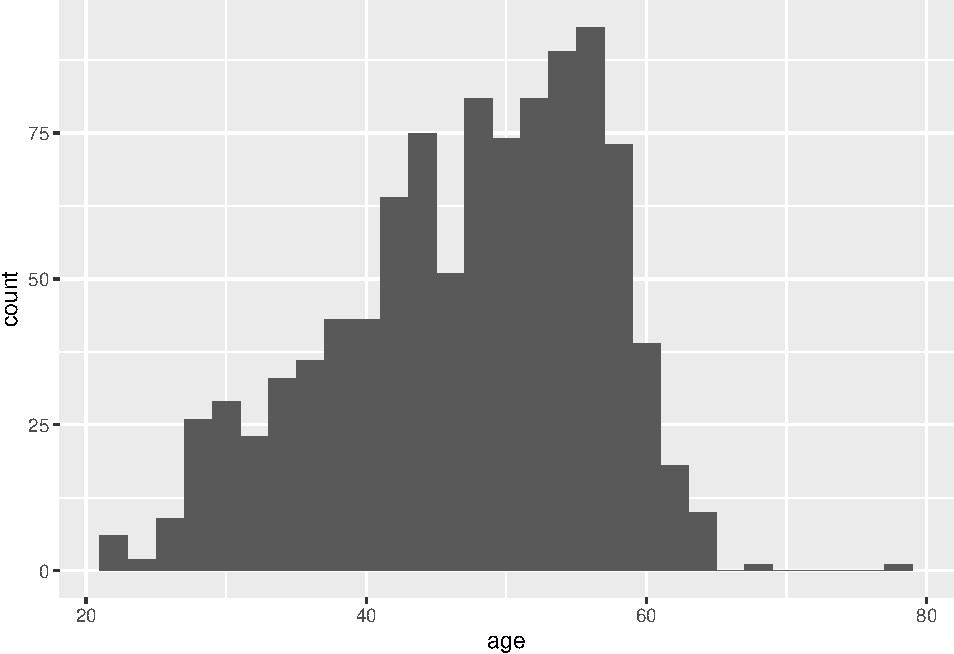
\includegraphics{R-for-social-research-and-business-analytics_files/figure-latex/unnamed-chunk-17-1.pdf}

Note that there is also a \emph{statistical transformation} being applied to the data before plotting (\emph{which one?}). We can modify that transformation of the data: for example, pick a different width for the histogram bins.

\begin{Shaded}
\begin{Highlighting}[]
\FunctionTok{ggplot}\NormalTok{(}\AttributeTok{data =}\NormalTok{ data) }\SpecialCharTok{+}
  \FunctionTok{geom\_histogram}\NormalTok{(}\FunctionTok{aes}\NormalTok{(}\AttributeTok{x =}\NormalTok{ age), }\AttributeTok{binwidth =} \DecValTok{1}\NormalTok{)}
\end{Highlighting}
\end{Shaded}

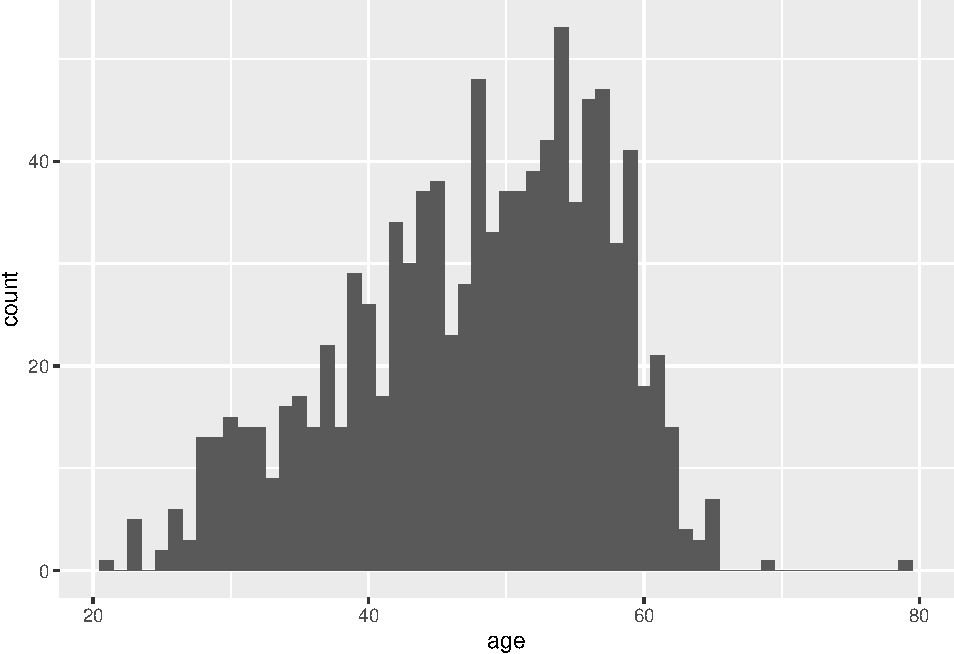
\includegraphics{R-for-social-research-and-business-analytics_files/figure-latex/unnamed-chunk-18-1.pdf}

Modify visual properties of the plot: bin color and fill.

\begin{Shaded}
\begin{Highlighting}[]
\FunctionTok{ggplot}\NormalTok{(}\AttributeTok{data =}\NormalTok{ data) }\SpecialCharTok{+}
  \FunctionTok{geom\_histogram}\NormalTok{(}\FunctionTok{aes}\NormalTok{(}\AttributeTok{x =}\NormalTok{ age), }\AttributeTok{binwidth =} \DecValTok{1}\NormalTok{,}
                 \AttributeTok{color =} \StringTok{"white"}\NormalTok{, }\AttributeTok{fill =} \StringTok{"black"}\NormalTok{)}
\end{Highlighting}
\end{Shaded}

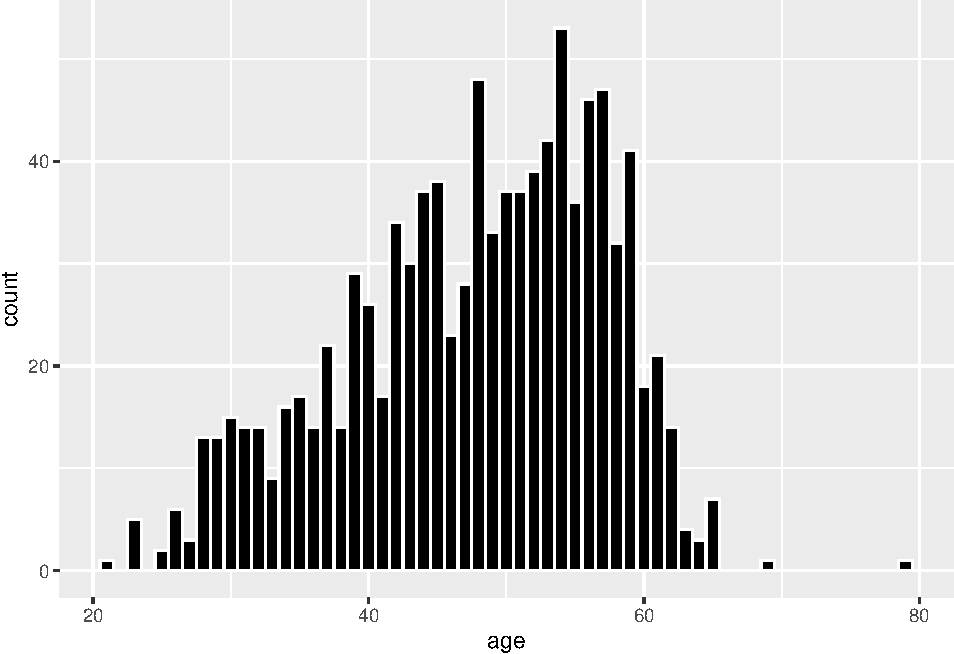
\includegraphics{R-for-social-research-and-business-analytics_files/figure-latex/unnamed-chunk-19-1.pdf}

Modify the scale of the \texttt{x} aesthetic mapping.

\begin{Shaded}
\begin{Highlighting}[]
\FunctionTok{ggplot}\NormalTok{(}\AttributeTok{data =}\NormalTok{ data) }\SpecialCharTok{+}
  \FunctionTok{geom\_histogram}\NormalTok{(}\FunctionTok{aes}\NormalTok{(}\AttributeTok{x =}\NormalTok{ age), }\AttributeTok{binwidth =} \DecValTok{1}\NormalTok{,}
                 \AttributeTok{color =} \StringTok{"white"}\NormalTok{, }\AttributeTok{fill =} \StringTok{"black"}\NormalTok{) }\SpecialCharTok{+}
  \FunctionTok{scale\_x\_continuous}\NormalTok{(}\AttributeTok{breaks =} \FunctionTok{seq}\NormalTok{(}\DecValTok{20}\NormalTok{, }\DecValTok{80}\NormalTok{, }\AttributeTok{by =} \DecValTok{10}\NormalTok{))}
\end{Highlighting}
\end{Shaded}

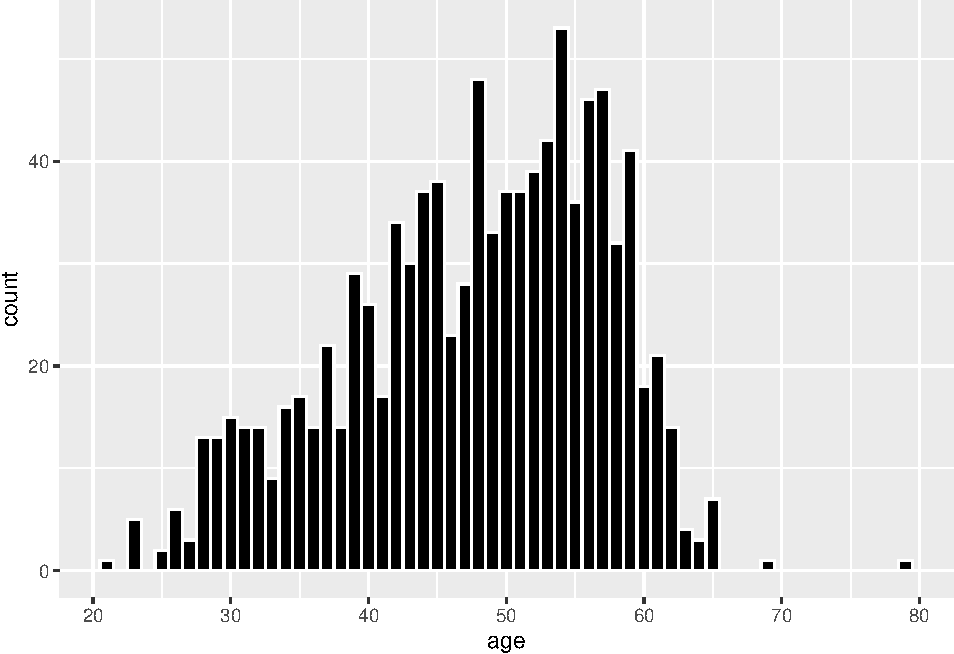
\includegraphics{R-for-social-research-and-business-analytics_files/figure-latex/unnamed-chunk-20-1.pdf}

Modify the general theme of the plot.

\begin{Shaded}
\begin{Highlighting}[]
\FunctionTok{ggplot}\NormalTok{(}\AttributeTok{data =}\NormalTok{ data) }\SpecialCharTok{+}
  \FunctionTok{geom\_histogram}\NormalTok{(}\FunctionTok{aes}\NormalTok{(}\AttributeTok{x =}\NormalTok{ age), }\AttributeTok{binwidth =} \DecValTok{1}\NormalTok{,}
                 \AttributeTok{color =} \StringTok{"white"}\NormalTok{, }\AttributeTok{fill =} \StringTok{"black"}\NormalTok{) }\SpecialCharTok{+}
  \FunctionTok{scale\_x\_continuous}\NormalTok{(}\AttributeTok{breaks =} \FunctionTok{seq}\NormalTok{(}\DecValTok{20}\NormalTok{, }\DecValTok{80}\NormalTok{, }\AttributeTok{by =} \DecValTok{10}\NormalTok{)) }\SpecialCharTok{+}
  \FunctionTok{theme\_bw}\NormalTok{()}
\end{Highlighting}
\end{Shaded}

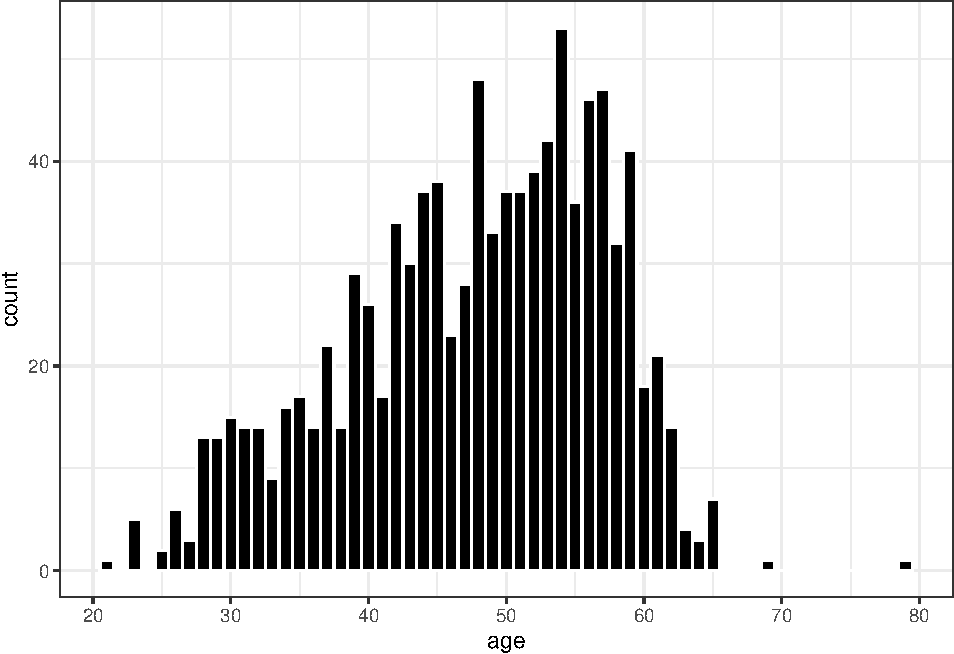
\includegraphics{R-for-social-research-and-business-analytics_files/figure-latex/unnamed-chunk-21-1.pdf}

Let's add another geom in a new layer: a density plot. Note that now the bin height and y axis are not count values but density values: this is specified by setting the \texttt{y} aesthetic in \texttt{aes()}.

\begin{Shaded}
\begin{Highlighting}[]
\FunctionTok{ggplot}\NormalTok{(}\AttributeTok{data =}\NormalTok{ data) }\SpecialCharTok{+}
  \FunctionTok{geom\_histogram}\NormalTok{(}\FunctionTok{aes}\NormalTok{(}\AttributeTok{x =}\NormalTok{ age, }\AttributeTok{y =} \FunctionTok{after\_stat}\NormalTok{(density)), }\AttributeTok{binwidth =} \DecValTok{1}\NormalTok{,}
                 \AttributeTok{color =} \StringTok{"white"}\NormalTok{, }\AttributeTok{fill =} \StringTok{"black"}\NormalTok{) }\SpecialCharTok{+}
  \FunctionTok{geom\_density}\NormalTok{(}\FunctionTok{aes}\NormalTok{(}\AttributeTok{x =}\NormalTok{ age), }\AttributeTok{linewidth =} \DecValTok{1}\NormalTok{, }\AttributeTok{color =} \StringTok{"red"}\NormalTok{) }\SpecialCharTok{+}
  \FunctionTok{scale\_x\_continuous}\NormalTok{(}\AttributeTok{breaks =} \FunctionTok{seq}\NormalTok{(}\DecValTok{20}\NormalTok{, }\DecValTok{80}\NormalTok{, }\AttributeTok{by =} \DecValTok{10}\NormalTok{)) }\SpecialCharTok{+}
  \FunctionTok{theme\_bw}\NormalTok{()}
\end{Highlighting}
\end{Shaded}

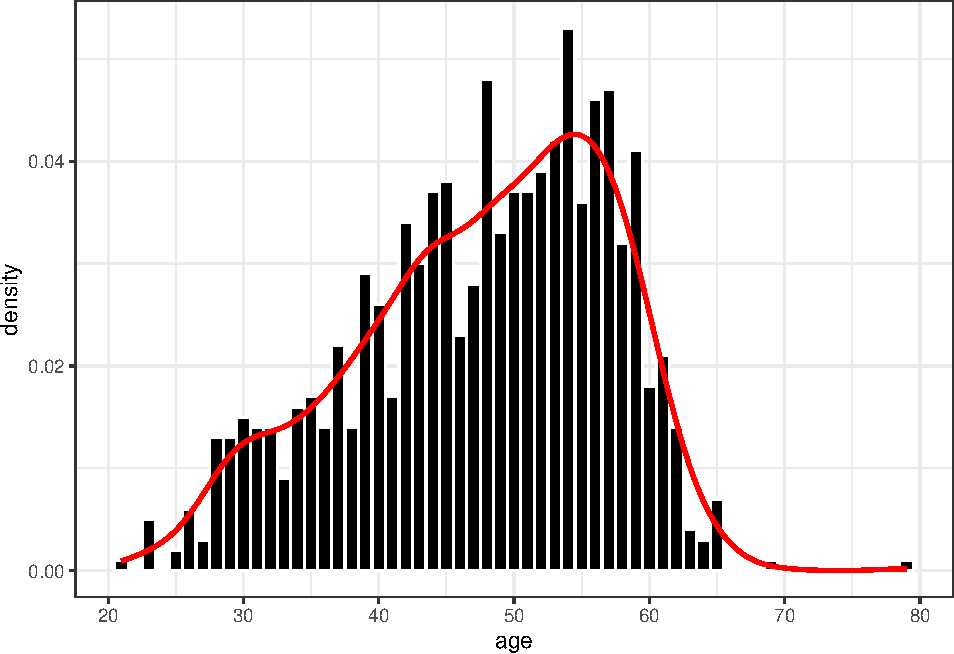
\includegraphics{R-for-social-research-and-business-analytics_files/figure-latex/unnamed-chunk-22-1.pdf}

\textbf{Boxplots.}

\begin{Shaded}
\begin{Highlighting}[]
\FunctionTok{ggplot}\NormalTok{(}\AttributeTok{data =}\NormalTok{ data) }\SpecialCharTok{+}
  \FunctionTok{geom\_boxplot}\NormalTok{(}\FunctionTok{aes}\NormalTok{(}\AttributeTok{x =}\NormalTok{ age))}
\end{Highlighting}
\end{Shaded}

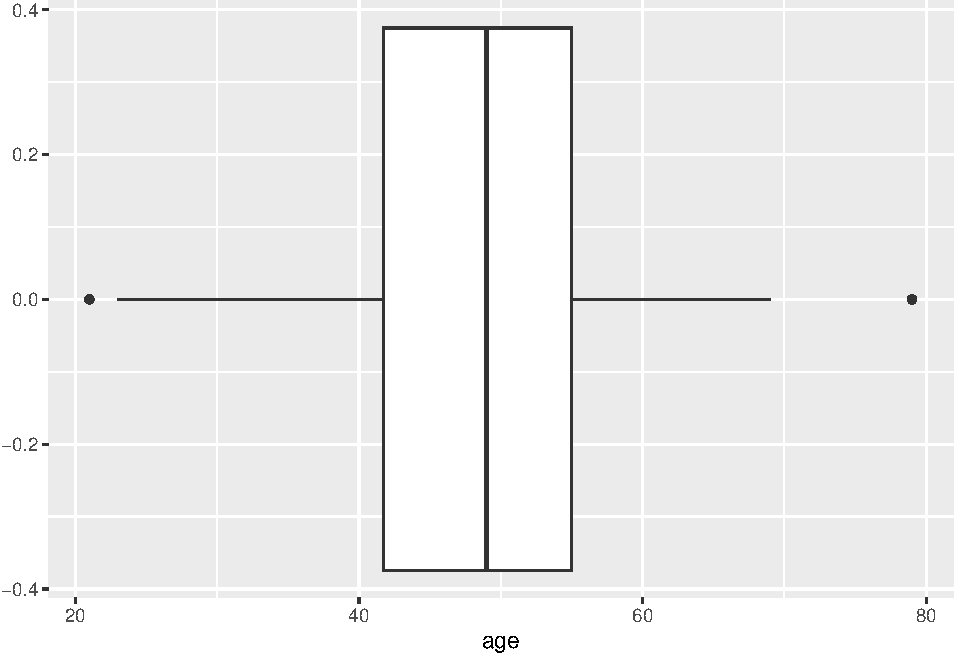
\includegraphics{R-for-social-research-and-business-analytics_files/figure-latex/unnamed-chunk-23-1.pdf}

In a new layer, we can use a new geom to add the actual data points on top of the boxplot (with some vertical jittering).

\begin{Shaded}
\begin{Highlighting}[]
\FunctionTok{set.seed}\NormalTok{(}\DecValTok{194}\NormalTok{)}
\FunctionTok{ggplot}\NormalTok{(}\AttributeTok{data =}\NormalTok{ data) }\SpecialCharTok{+}
  \FunctionTok{geom\_point}\NormalTok{(}\FunctionTok{aes}\NormalTok{(}\AttributeTok{x =}\NormalTok{ age, }\AttributeTok{y =} \DecValTok{0}\NormalTok{), }
             \AttributeTok{shape =} \DecValTok{21}\NormalTok{,}
             \AttributeTok{position =} \FunctionTok{position\_jitter}\NormalTok{(}\AttributeTok{h =} \FloatTok{0.2}\NormalTok{)) }\SpecialCharTok{+}
  \FunctionTok{geom\_boxplot}\NormalTok{(}\FunctionTok{aes}\NormalTok{(}\AttributeTok{x =}\NormalTok{ age), }\AttributeTok{fill =} \ConstantTok{NA}\NormalTok{, }\AttributeTok{color =} \StringTok{"red"}\NormalTok{)}
\end{Highlighting}
\end{Shaded}

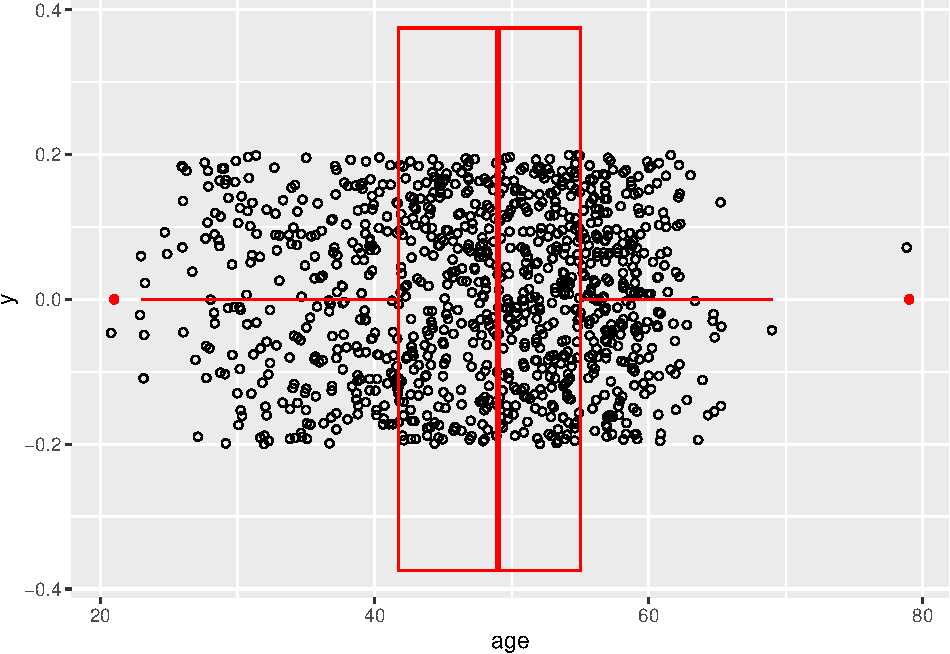
\includegraphics{R-for-social-research-and-business-analytics_files/figure-latex/unnamed-chunk-24-1.pdf}

\hypertarget{categorical-variables-simple-barplots}{%
\subsection{Categorical variables: simple barplots}\label{categorical-variables-simple-barplots}}

\textbf{Simple barplots}.

\begin{Shaded}
\begin{Highlighting}[]
\FunctionTok{ggplot}\NormalTok{(}\AttributeTok{data =}\NormalTok{ data) }\SpecialCharTok{+}
  \FunctionTok{geom\_bar}\NormalTok{(}\FunctionTok{aes}\NormalTok{(}\AttributeTok{x =}\NormalTok{ edu))}
\end{Highlighting}
\end{Shaded}

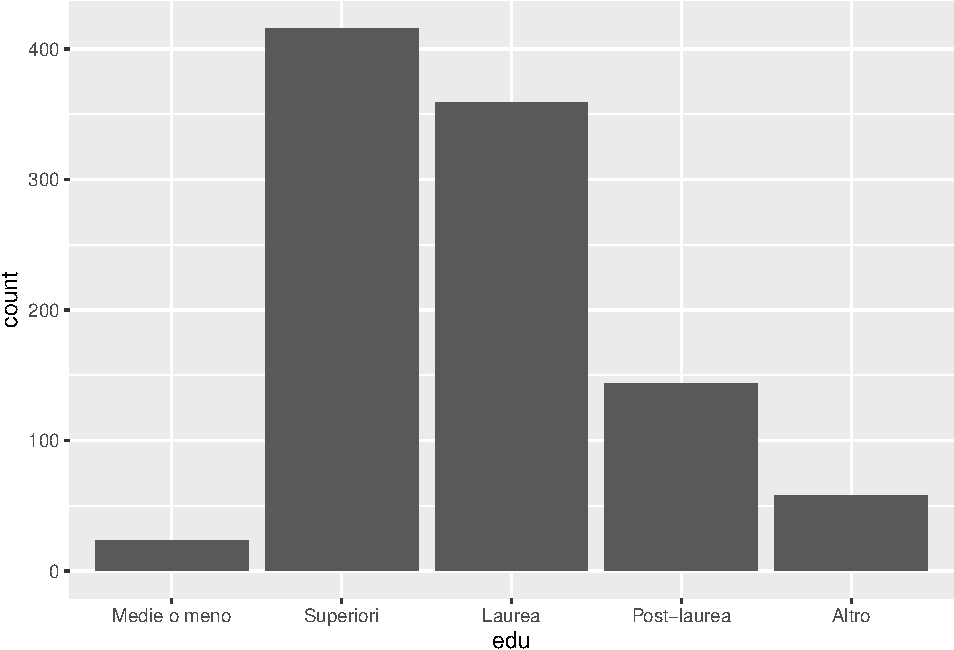
\includegraphics{R-for-social-research-and-business-analytics_files/figure-latex/unnamed-chunk-25-1.pdf}

Two aesthetics (\texttt{x} and \texttt{fill}) for the same variable (\texttt{edu}).

\begin{Shaded}
\begin{Highlighting}[]
\FunctionTok{ggplot}\NormalTok{(}\AttributeTok{data =}\NormalTok{ data) }\SpecialCharTok{+}
  \FunctionTok{geom\_bar}\NormalTok{(}\FunctionTok{aes}\NormalTok{(}\AttributeTok{x =}\NormalTok{ edu, }\AttributeTok{fill =}\NormalTok{ edu))}
\end{Highlighting}
\end{Shaded}

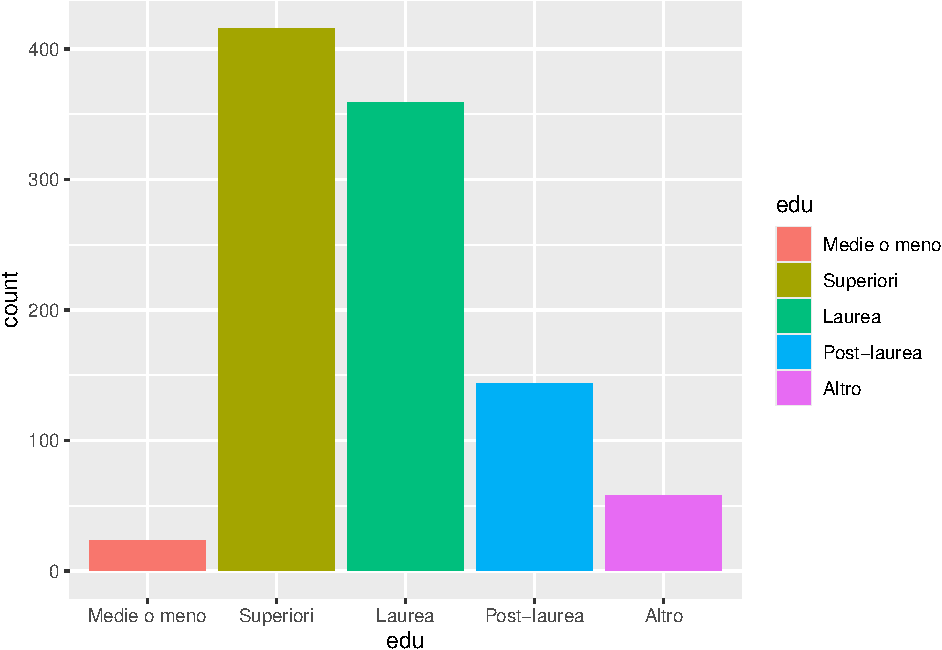
\includegraphics{R-for-social-research-and-business-analytics_files/figure-latex/unnamed-chunk-26-1.pdf}

Note the importance of the order of levels in \texttt{edu} factor.

\begin{Shaded}
\begin{Highlighting}[]
\CommentTok{\# Original level order}
\NormalTok{data}\SpecialCharTok{$}\NormalTok{edu }\SpecialCharTok{|\textgreater{}} 
  \FunctionTok{levels}\NormalTok{()}
\end{Highlighting}
\end{Shaded}

\begin{verbatim}
## [1] "Medie o meno" "Superiori"    "Laurea"       "Post-laurea"  "Altro"
\end{verbatim}

\begin{Shaded}
\begin{Highlighting}[]
\CommentTok{\# Let\textquotesingle{}s change it to this:}
\NormalTok{data}\SpecialCharTok{$}\NormalTok{edu }\SpecialCharTok{|\textgreater{}}
  \FunctionTok{fct\_rev}\NormalTok{() }\SpecialCharTok{|\textgreater{}} 
  \FunctionTok{levels}\NormalTok{()}
\end{Highlighting}
\end{Shaded}

\begin{verbatim}
## [1] "Altro"        "Post-laurea"  "Laurea"       "Superiori"    "Medie o meno"
\end{verbatim}

\begin{Shaded}
\begin{Highlighting}[]
\CommentTok{\# Make the change in the data}
\NormalTok{data.rev }\OtherTok{\textless{}{-}}\NormalTok{ data }\SpecialCharTok{|\textgreater{}} 
  \FunctionTok{mutate}\NormalTok{(}\AttributeTok{edu =} \FunctionTok{fct\_rev}\NormalTok{(edu))}

\CommentTok{\# Not plot with the new level order}
\FunctionTok{ggplot}\NormalTok{(}\AttributeTok{data =}\NormalTok{ data.rev) }\SpecialCharTok{+}
  \FunctionTok{geom\_bar}\NormalTok{(}\FunctionTok{aes}\NormalTok{(}\AttributeTok{x =}\NormalTok{ edu, }\AttributeTok{fill =}\NormalTok{ edu))}
\end{Highlighting}
\end{Shaded}

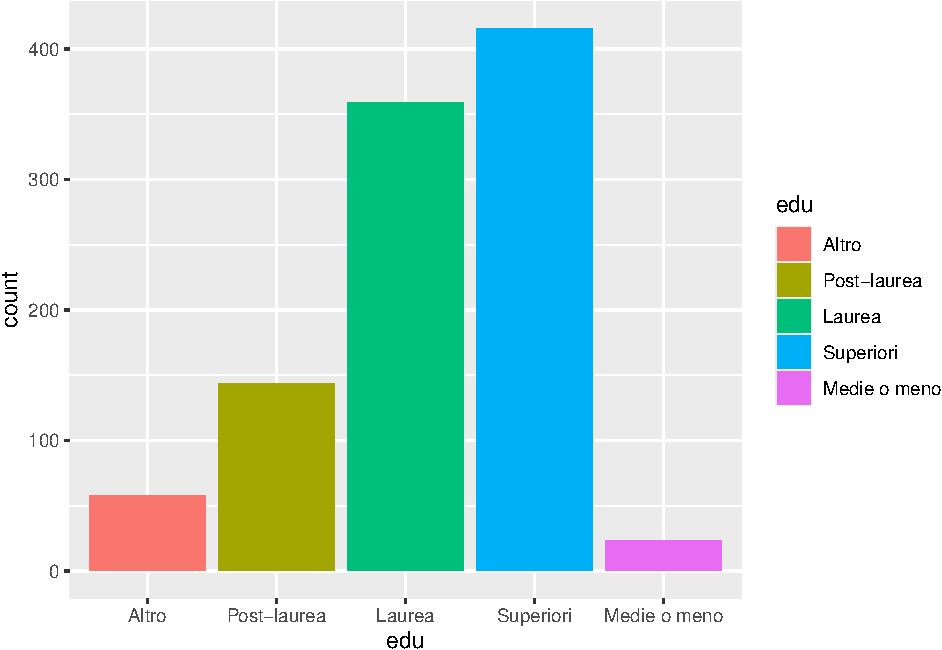
\includegraphics{R-for-social-research-and-business-analytics_files/figure-latex/unnamed-chunk-27-1.pdf}

Back to the original level order, modify the fill color scale (and theme).

\begin{Shaded}
\begin{Highlighting}[]
\FunctionTok{ggplot}\NormalTok{(}\AttributeTok{data =}\NormalTok{ data) }\SpecialCharTok{+}
  \FunctionTok{geom\_bar}\NormalTok{(}\FunctionTok{aes}\NormalTok{(}\AttributeTok{x =}\NormalTok{ edu, }\AttributeTok{fill =}\NormalTok{ edu)) }\SpecialCharTok{+}
  \FunctionTok{scale\_fill\_manual}\NormalTok{(}\AttributeTok{values =} \FunctionTok{c}\NormalTok{(}\StringTok{\textasciigrave{}}\AttributeTok{Medie o meno}\StringTok{\textasciigrave{}} \OtherTok{=} \StringTok{"\#002e4e"}\NormalTok{, }
                               \AttributeTok{Superiori =} \StringTok{"\#afe1da"}\NormalTok{, }
                               \AttributeTok{Laurea =} \StringTok{"\#ff4639"}\NormalTok{, }
                               \StringTok{\textasciigrave{}}\AttributeTok{Post{-}laurea}\StringTok{\textasciigrave{}} \OtherTok{=} \StringTok{"\#b4abd7"}\NormalTok{, }
                               \AttributeTok{Altro =} \StringTok{"\#fad774"}\NormalTok{)) }\SpecialCharTok{+}
  \FunctionTok{theme\_minimal}\NormalTok{()}
\end{Highlighting}
\end{Shaded}

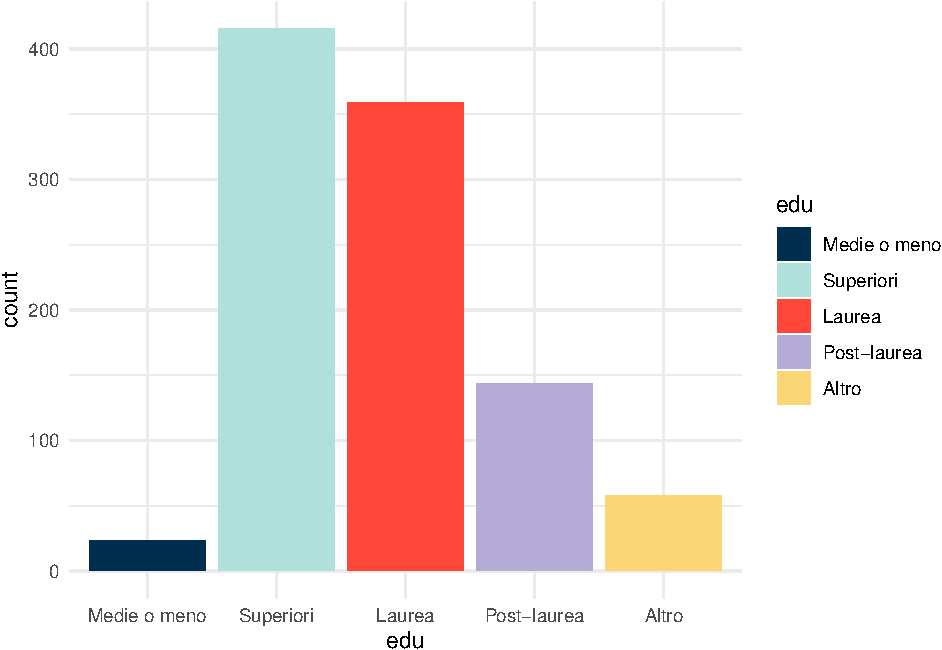
\includegraphics{R-for-social-research-and-business-analytics_files/figure-latex/unnamed-chunk-28-1.pdf}

\hypertarget{associations-between-two-variables}{%
\section{Associations between two variables}\label{associations-between-two-variables}}

\hypertarget{two-continuous-variables-scatterplots}{%
\subsection{Two continuous variables: scatterplots}\label{two-continuous-variables-scatterplots}}

Let's first consider the association between \texttt{age} and \texttt{work.exp.y} (years of experience in current company). We expect a positive association

\begin{Shaded}
\begin{Highlighting}[]
\FunctionTok{ggplot}\NormalTok{(}\AttributeTok{data =}\NormalTok{ data) }\SpecialCharTok{+}
  \FunctionTok{geom\_point}\NormalTok{(}\FunctionTok{aes}\NormalTok{(}\AttributeTok{x =}\NormalTok{ age, }\AttributeTok{y =}\NormalTok{ work.exp.y))}
\end{Highlighting}
\end{Shaded}

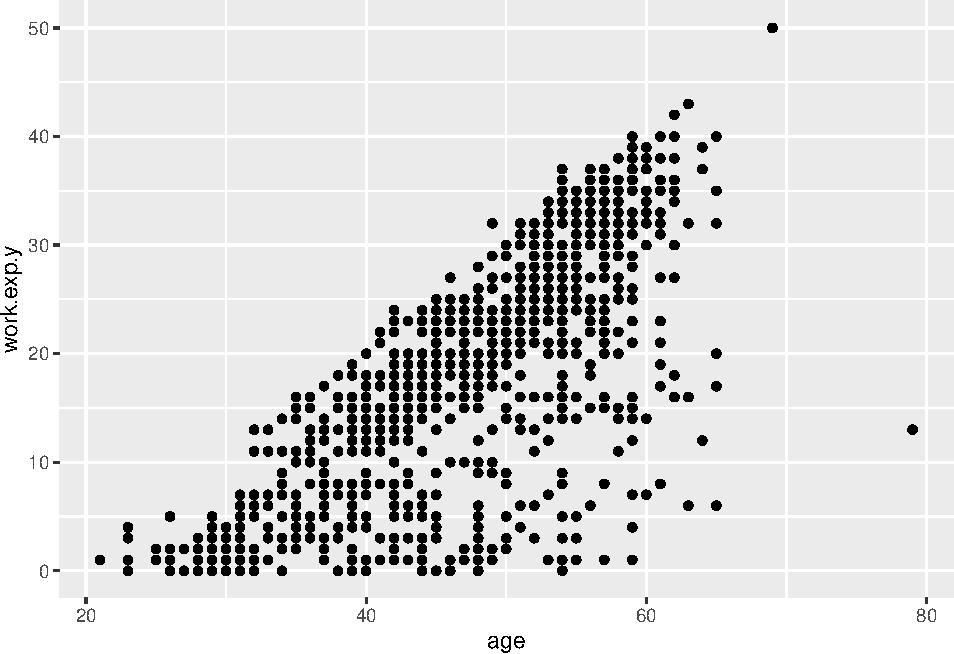
\includegraphics{R-for-social-research-and-business-analytics_files/figure-latex/unnamed-chunk-29-1.pdf}

Note that there is a lot of overplotting: many of those dots represent multiple data points (what makes us suspicious about this is that points are too neatly arranged as in a grid). Indeed, for each unique combination of \texttt{age} and \texttt{work.exp.y} there are multiple data points (i.e.~multiple respondents):

\begin{Shaded}
\begin{Highlighting}[]
\NormalTok{data }\SpecialCharTok{|\textgreater{}} 
  \FunctionTok{group\_by}\NormalTok{(age, work.exp.y) }\SpecialCharTok{|\textgreater{}} 
  \FunctionTok{count}\NormalTok{() }\SpecialCharTok{|\textgreater{}} 
  \FunctionTok{arrange}\NormalTok{(}\FunctionTok{desc}\NormalTok{(n))}
\end{Highlighting}
\end{Shaded}

\begin{verbatim}
## # A tibble: 530 x 3
## # Groups:   age, work.exp.y [530]
##      age work.exp.y     n
##    <dbl>      <dbl> <int>
##  1    51         30     7
##  2    53         32     7
##  3    54         32     7
##  4    56         35     7
##  5    30          2     6
##  6    42         15     6
##  7    49         22     6
##  8    56         30     6
##  9    57         33     6
## 10    57         35     6
## # i 520 more rows
\end{verbatim}

To see this more clearly in the plot, we can change point shape to hollow point and add a little horizontal jittering.

\begin{Shaded}
\begin{Highlighting}[]
\FunctionTok{set.seed}\NormalTok{(}\DecValTok{106}\NormalTok{)}
\FunctionTok{ggplot}\NormalTok{(}\AttributeTok{data =}\NormalTok{ data) }\SpecialCharTok{+}
  \FunctionTok{geom\_point}\NormalTok{(}\FunctionTok{aes}\NormalTok{(}\AttributeTok{x =}\NormalTok{ age, }\AttributeTok{y =}\NormalTok{ work.exp.y), }\AttributeTok{shape =} \DecValTok{21}\NormalTok{, }\AttributeTok{position =} \FunctionTok{position\_jitter}\NormalTok{(}\AttributeTok{w =} \FloatTok{0.3}\NormalTok{))}
\end{Highlighting}
\end{Shaded}

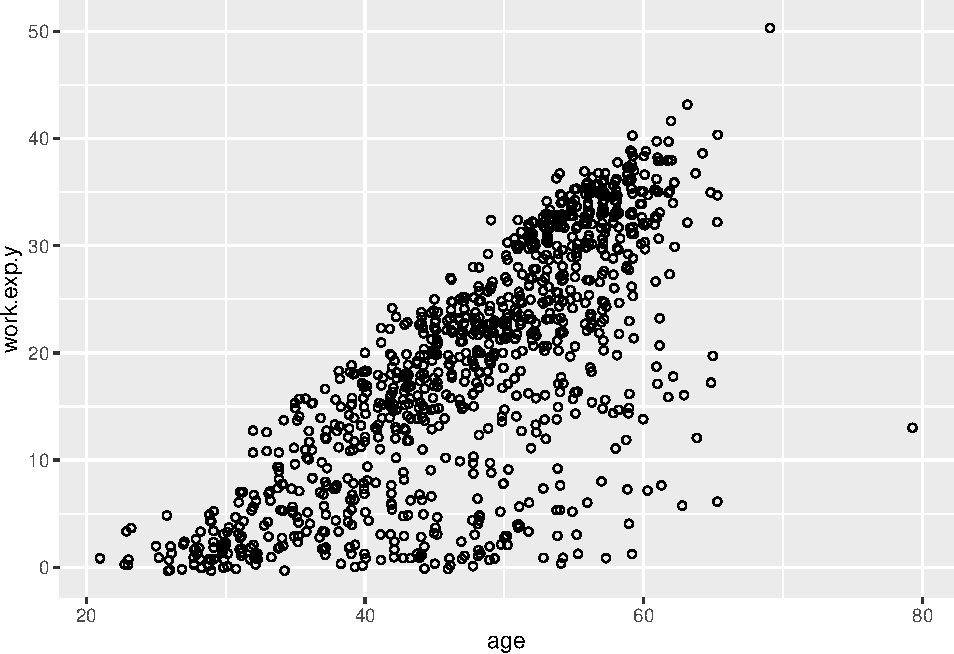
\includegraphics{R-for-social-research-and-business-analytics_files/figure-latex/unnamed-chunk-31-1.pdf}

The positive association between the \emph{x} and \emph{y} variables can be seen more clearly if we add, in a new layer, the smoothing line that best approximates the relationship between \emph{x} and \emph{y}. Note that now we have two geoms with the same \texttt{aes()} argument, so we move \texttt{aes()} into the \texttt{ggplot()} call to avoid having to repeat it in both geom calls.

\begin{Shaded}
\begin{Highlighting}[]
\FunctionTok{set.seed}\NormalTok{(}\DecValTok{106}\NormalTok{)}
\FunctionTok{ggplot}\NormalTok{(}\AttributeTok{data =}\NormalTok{ data, }\FunctionTok{aes}\NormalTok{(}\AttributeTok{x =}\NormalTok{ age, }\AttributeTok{y =}\NormalTok{ work.exp.y)) }\SpecialCharTok{+}
  \FunctionTok{geom\_point}\NormalTok{(}\AttributeTok{shape =} \DecValTok{21}\NormalTok{, }\AttributeTok{position =} \FunctionTok{position\_jitter}\NormalTok{(}\AttributeTok{w =} \FloatTok{0.3}\NormalTok{)) }\SpecialCharTok{+}
  \FunctionTok{geom\_smooth}\NormalTok{()}
\end{Highlighting}
\end{Shaded}

\begin{verbatim}
## `geom_smooth()` using method = 'gam' and formula = 'y ~ s(x, bs = "cs")'
\end{verbatim}

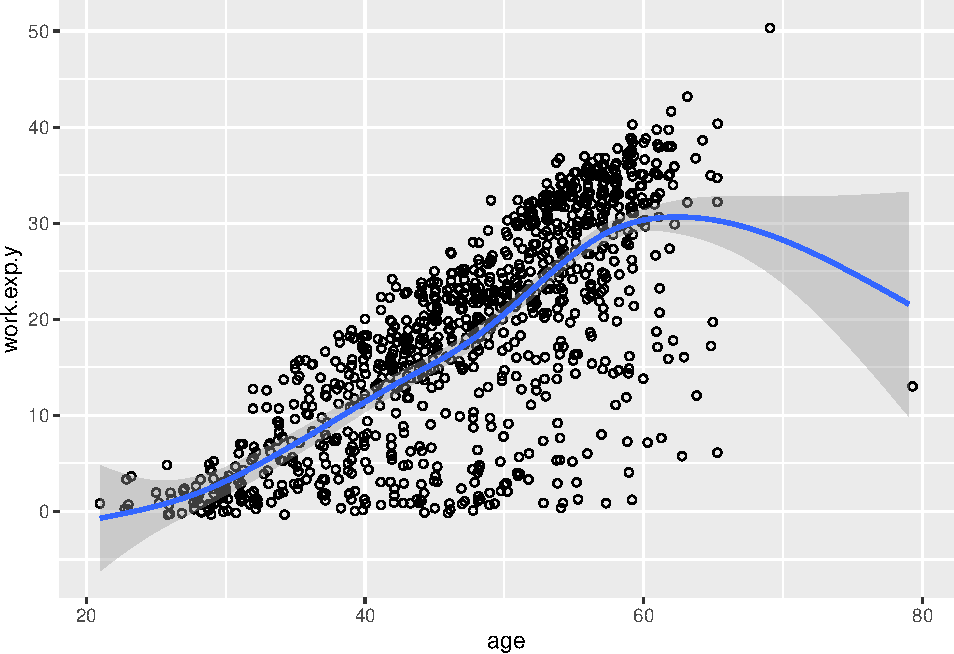
\includegraphics{R-for-social-research-and-business-analytics_files/figure-latex/unnamed-chunk-32-1.pdf}

Let's do the same plot for another pair of continuous variables: \texttt{age} and \texttt{driver.sum}. The latter is the sum of all answers (converted to numeric) to the 24 ``driver'' questions: an overall score of a respondent's tendency to agree that the ``drivers'' listed in the survey are important. We'll change colors and theme just to show some graphical variation.

\begin{Shaded}
\begin{Highlighting}[]
\FunctionTok{set.seed}\NormalTok{(}\DecValTok{106}\NormalTok{)}
\FunctionTok{ggplot}\NormalTok{(}\AttributeTok{data =}\NormalTok{ data, }\FunctionTok{aes}\NormalTok{(}\AttributeTok{x =}\NormalTok{ age, }\AttributeTok{y =}\NormalTok{ driver.sum)) }\SpecialCharTok{+}
  \FunctionTok{geom\_point}\NormalTok{(}\AttributeTok{shape =} \DecValTok{21}\NormalTok{, }\AttributeTok{color =} \StringTok{"white"}\NormalTok{, }\AttributeTok{position =} \FunctionTok{position\_jitter}\NormalTok{(}\AttributeTok{w =} \FloatTok{0.3}\NormalTok{)) }\SpecialCharTok{+}
  \FunctionTok{geom\_smooth}\NormalTok{(}\AttributeTok{color =} \StringTok{"red"}\NormalTok{) }\SpecialCharTok{+}
  \FunctionTok{theme\_dark}\NormalTok{()}
\end{Highlighting}
\end{Shaded}

\begin{verbatim}
## `geom_smooth()` using method = 'gam' and formula = 'y ~ s(x, bs = "cs")'
\end{verbatim}

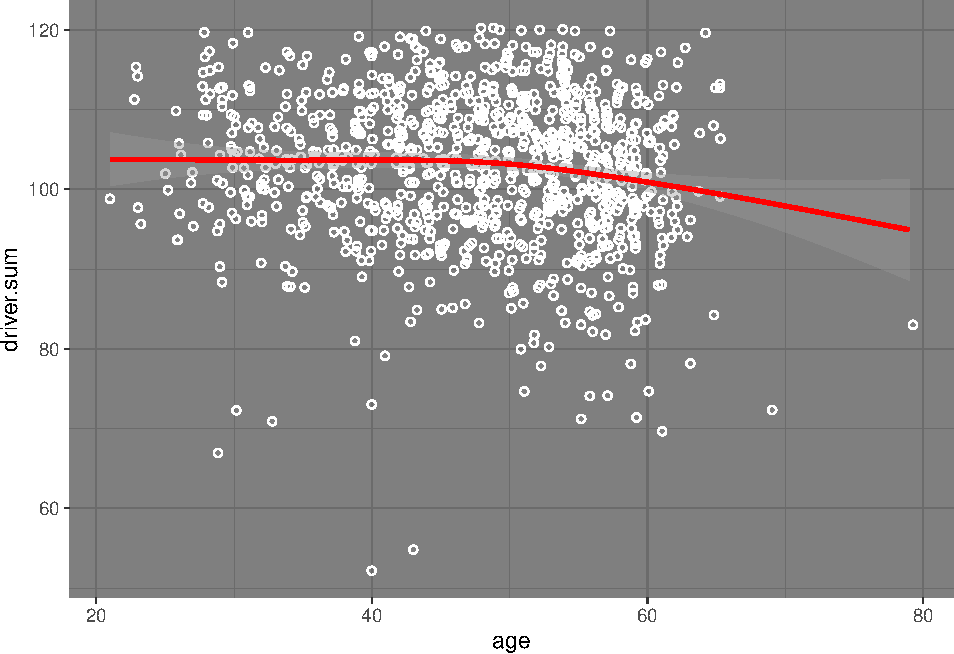
\includegraphics{R-for-social-research-and-business-analytics_files/figure-latex/unnamed-chunk-33-1.pdf}

\hypertarget{two-categorical-variables-complex-barplots}{%
\subsection{Two categorical variables: complex barplots}\label{two-categorical-variables-complex-barplots}}

Here we want to visualize the relationship between two categorical variables: generation (\texttt{gen}) and education level (\texttt{edu}). You can think of the data we want to view as a table of counts (\emph{absolute frequencies}) of \texttt{edu} categories in each \texttt{gen} category:

\begin{Shaded}
\begin{Highlighting}[]
\NormalTok{data }\SpecialCharTok{|\textgreater{}} 
  \FunctionTok{tabyl}\NormalTok{(edu, gen) }
\end{Highlighting}
\end{Shaded}

\begin{verbatim}
##           edu baby boomers gen x millennials gen z
##  Medie o meno            3    18           2     0
##     Superiori           62   289          62     3
##        Laurea           34   166         149    10
##   Post-laurea            4    66          71     3
##         Altro            7    37          13     1
\end{verbatim}

We can also think of the data as \emph{relative frequencies} of \texttt{edu} categories in each \texttt{gen} category:

\begin{Shaded}
\begin{Highlighting}[]
\NormalTok{data }\SpecialCharTok{|\textgreater{}} 
  \FunctionTok{tabyl}\NormalTok{(edu, gen) }\SpecialCharTok{|\textgreater{}} 
  \FunctionTok{adorn\_percentages}\NormalTok{(}\AttributeTok{denominator =} \StringTok{"col"}\NormalTok{) }\SpecialCharTok{|\textgreater{}} 
  \FunctionTok{adorn\_rounding}\NormalTok{(}\DecValTok{2}\NormalTok{)}
\end{Highlighting}
\end{Shaded}

\begin{verbatim}
##           edu baby boomers gen x millennials gen z
##  Medie o meno         0.03  0.03        0.01  0.00
##     Superiori         0.56  0.50        0.21  0.18
##        Laurea         0.31  0.29        0.50  0.59
##   Post-laurea         0.04  0.11        0.24  0.18
##         Altro         0.06  0.06        0.04  0.06
\end{verbatim}

Alternatively, we can look at the relative frequencies of \texttt{gen} categories in each \texttt{edu} category:

\begin{Shaded}
\begin{Highlighting}[]
\NormalTok{data }\SpecialCharTok{|\textgreater{}} 
  \FunctionTok{tabyl}\NormalTok{(edu, gen) }\SpecialCharTok{|\textgreater{}} 
  \FunctionTok{adorn\_percentages}\NormalTok{(}\AttributeTok{denominator =} \StringTok{"row"}\NormalTok{) }\SpecialCharTok{|\textgreater{}} 
  \FunctionTok{adorn\_rounding}\NormalTok{(}\DecValTok{2}\NormalTok{)}
\end{Highlighting}
\end{Shaded}

\begin{verbatim}
##           edu baby boomers gen x millennials gen z
##  Medie o meno         0.13  0.78        0.09  0.00
##     Superiori         0.15  0.69        0.15  0.01
##        Laurea         0.09  0.46        0.42  0.03
##   Post-laurea         0.03  0.46        0.49  0.02
##         Altro         0.12  0.64        0.22  0.02
\end{verbatim}

\textbf{Grouped barplots.}

We start by plotting the counts of educational categories in each generation. Here, each bar is an educational category \emph{within} a generation category. Bars are grouped by generation: each generation is a group with one position on the x axis, and all bars for one generation are plotted side by side around that generation's x position. Note that we transform \texttt{gen} with \texttt{fct\_rev()} so as to have younger generations first, that is, younger on the left and older on the right (the transformation is done within the plot, it doesn't affect the \texttt{data} object).

\begin{Shaded}
\begin{Highlighting}[]
\FunctionTok{ggplot}\NormalTok{(}\AttributeTok{data =}\NormalTok{ data) }\SpecialCharTok{+}
  \FunctionTok{geom\_bar}\NormalTok{(}\FunctionTok{aes}\NormalTok{(}\AttributeTok{x =} \FunctionTok{fct\_rev}\NormalTok{(gen), }\AttributeTok{fill =}\NormalTok{ edu), }\AttributeTok{position =} \StringTok{"dodge"}\NormalTok{)}
\end{Highlighting}
\end{Shaded}

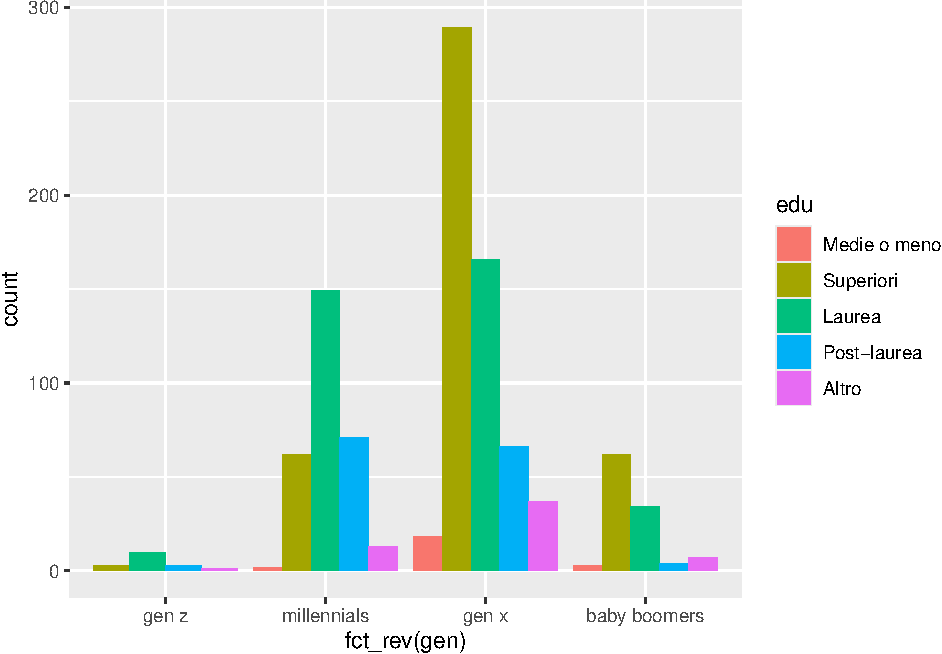
\includegraphics{R-for-social-research-and-business-analytics_files/figure-latex/unnamed-chunk-37-1.pdf}

The \texttt{position\ =\ "dodge"} argument is what tells R to put the different \texttt{edu} bars in the same \texttt{gen} category side by side. We can invert \texttt{gen} and \texttt{edu}, by setting \texttt{edu} as the group and x position, and \texttt{gen} as the categories to be plotted side by side in the same \texttt{edu} group:

\begin{Shaded}
\begin{Highlighting}[]
\FunctionTok{ggplot}\NormalTok{(}\AttributeTok{data =}\NormalTok{ data) }\SpecialCharTok{+}
  \FunctionTok{geom\_bar}\NormalTok{(}\FunctionTok{aes}\NormalTok{(}\AttributeTok{x =}\NormalTok{ edu, }\AttributeTok{fill =} \FunctionTok{fct\_rev}\NormalTok{(gen)), }\AttributeTok{position =} \StringTok{"dodge"}\NormalTok{)}
\end{Highlighting}
\end{Shaded}

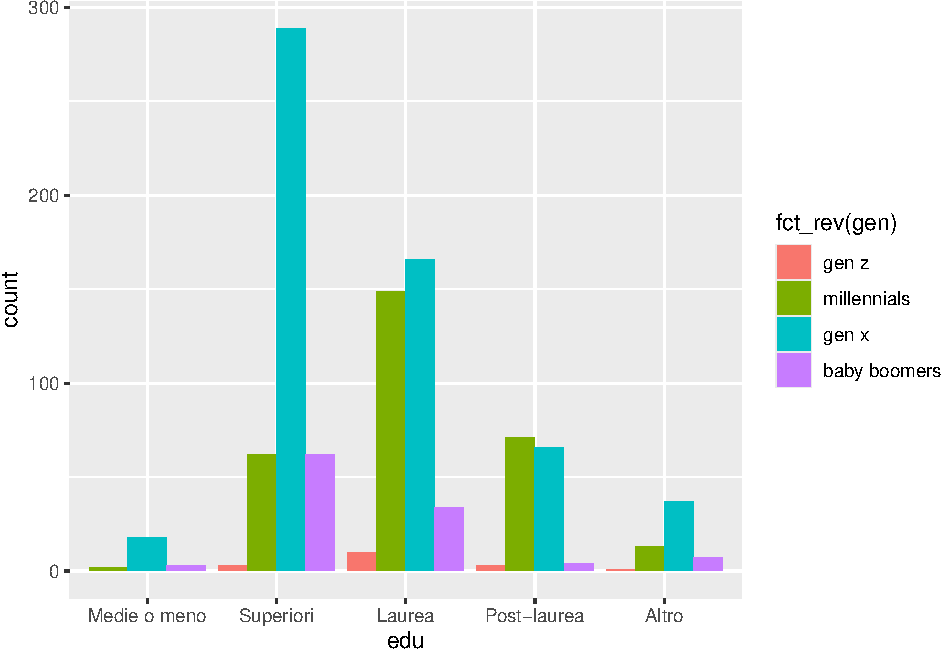
\includegraphics{R-for-social-research-and-business-analytics_files/figure-latex/unnamed-chunk-38-1.pdf}

If we omit the \texttt{position} argument, the bars will be plotted one on top of the other: a stacked barplot.

\textbf{Stacked barplots.}

\begin{Shaded}
\begin{Highlighting}[]
\FunctionTok{ggplot}\NormalTok{(}\AttributeTok{data =}\NormalTok{ data) }\SpecialCharTok{+}
  \FunctionTok{geom\_bar}\NormalTok{(}\FunctionTok{aes}\NormalTok{(}\AttributeTok{x =} \FunctionTok{fct\_rev}\NormalTok{(gen), }\AttributeTok{fill =}\NormalTok{ edu))}
\end{Highlighting}
\end{Shaded}

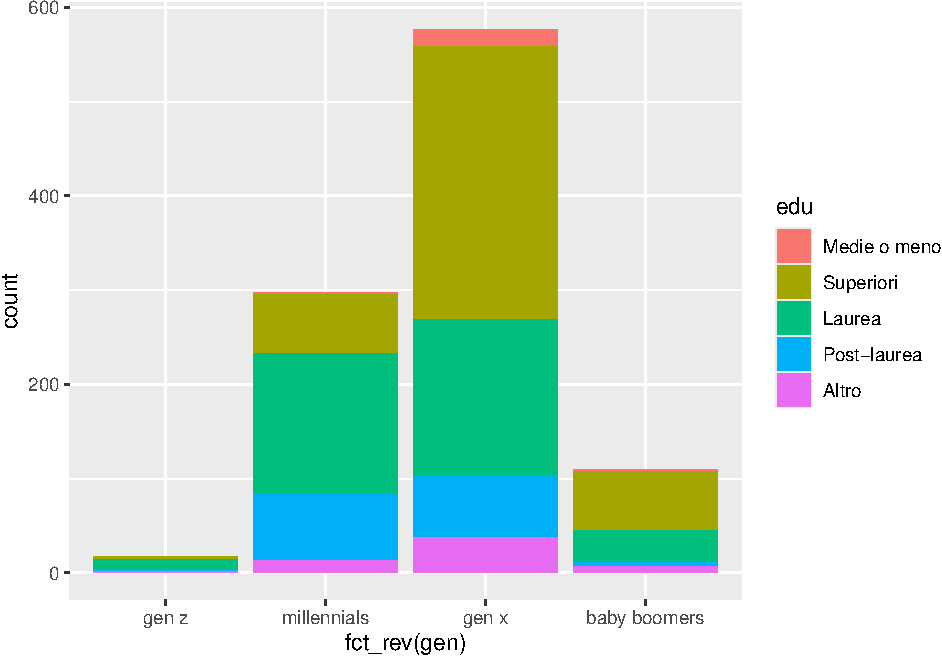
\includegraphics{R-for-social-research-and-business-analytics_files/figure-latex/unnamed-chunk-39-1.pdf}

Note that these are counts: we are not seeing the relative frequencies of \texttt{edu} categories within each generation, and generations with more respondents (e.g., Gen X) correspond to taller bars (counts are larger).

To get relative frequencies (i.e.~proportions or percentages) in each generation, standardizing all bar heights to the same (1 or 100), we set the \texttt{position} argument to \texttt{"fill"}. Now we see a clear pattern of association between generation and education level.

\begin{Shaded}
\begin{Highlighting}[]
\FunctionTok{ggplot}\NormalTok{(}\AttributeTok{data =}\NormalTok{ data) }\SpecialCharTok{+}
  \FunctionTok{geom\_bar}\NormalTok{(}\FunctionTok{aes}\NormalTok{(}\AttributeTok{x =} \FunctionTok{fct\_rev}\NormalTok{(gen), }\AttributeTok{fill =}\NormalTok{ edu), }\AttributeTok{position =} \StringTok{"fill"}\NormalTok{)}
\end{Highlighting}
\end{Shaded}

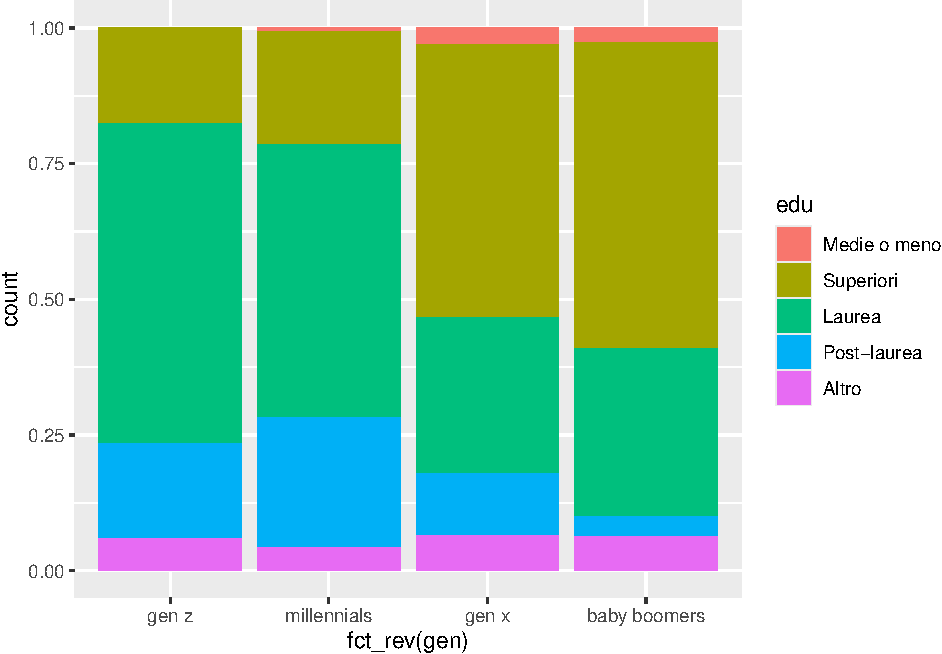
\includegraphics{R-for-social-research-and-business-analytics_files/figure-latex/unnamed-chunk-40-1.pdf}

\hypertarget{one-continuous-and-one-categorical-variable-boxplots-and-faceted-histograms}{%
\subsection{One continuous and one categorical variable: boxplots and faceted histograms}\label{one-continuous-and-one-categorical-variable-boxplots-and-faceted-histograms}}

\textbf{Boxplots.}

We have already seen boxplots. Since a boxplot is a very parsimonious and concise way of displaying a univariate distribution, we can easily draw multiple boxplots -- one for each group -- to compare the univariate distribution of the same variable (e.g., \texttt{driver.sum}) in different groups (e.g., generations) side by side. All we need is set the continous variable as the \emph{x} aesthetic and the categorical variable as the \emph{y} (or viceversa for vertical boxplots):

\begin{Shaded}
\begin{Highlighting}[]
\FunctionTok{ggplot}\NormalTok{(}\AttributeTok{data =}\NormalTok{ data) }\SpecialCharTok{+}
  \FunctionTok{geom\_boxplot}\NormalTok{(}\FunctionTok{aes}\NormalTok{(}\AttributeTok{x =}\NormalTok{ driver.sum, }\AttributeTok{y =}\NormalTok{ gen))}
\end{Highlighting}
\end{Shaded}

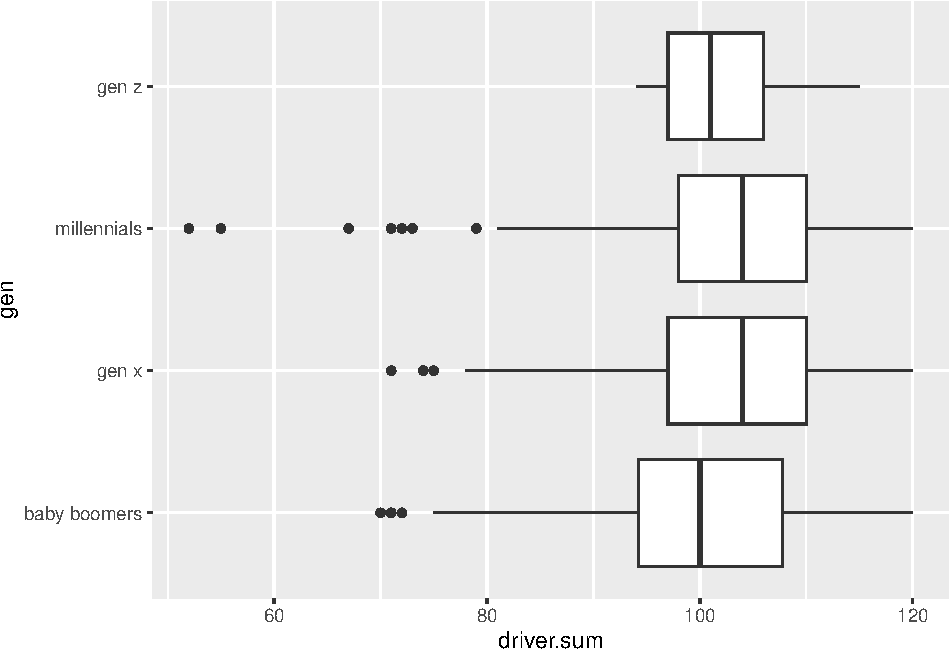
\includegraphics{R-for-social-research-and-business-analytics_files/figure-latex/unnamed-chunk-41-1.pdf}

We do see some pattern here (\emph{what is that?}).

\textbf{Faceted histograms.}

Whenever we have a categorical variable, we can use \textbf{facets} to create the same plot for each group (i.e., category) of that categorical variable. In other words, the same plot will have multiple facets, each facet corresponding to one category. In this way, we can create, for example, the same histogram of \texttt{driver.sum} for each \texttt{gen} category separately. Let's start by creating the one \texttt{driver.sum} histogram we want:

\begin{Shaded}
\begin{Highlighting}[]
\FunctionTok{ggplot}\NormalTok{(}\AttributeTok{data =}\NormalTok{ data) }\SpecialCharTok{+}
  \FunctionTok{geom\_histogram}\NormalTok{(}\FunctionTok{aes}\NormalTok{(}\AttributeTok{x =}\NormalTok{ driver.sum, }\AttributeTok{y =} \FunctionTok{after\_stat}\NormalTok{(density)), }\AttributeTok{binwidth =} \DecValTok{5}\NormalTok{, }\AttributeTok{color =} \StringTok{"white"}\NormalTok{) }\SpecialCharTok{+}
  \FunctionTok{theme\_bw}\NormalTok{()}
\end{Highlighting}
\end{Shaded}

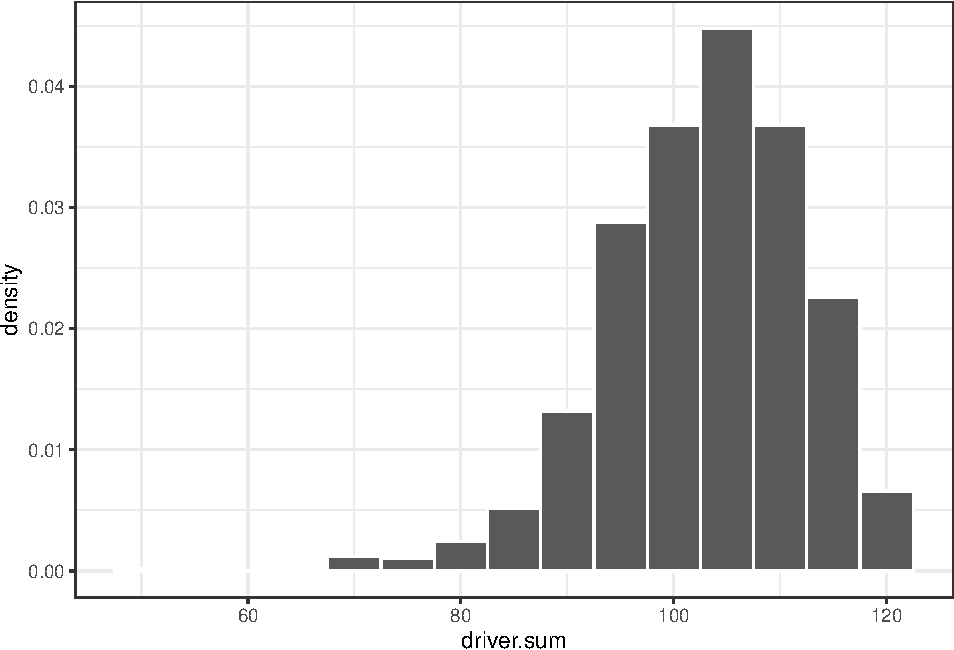
\includegraphics{R-for-social-research-and-business-analytics_files/figure-latex/unnamed-chunk-42-1.pdf}

By adding a facet function, we can now create the same plot for each facet (e.g., \texttt{gen} category):

\begin{Shaded}
\begin{Highlighting}[]
\FunctionTok{ggplot}\NormalTok{(}\AttributeTok{data =}\NormalTok{ data) }\SpecialCharTok{+}
  \FunctionTok{geom\_histogram}\NormalTok{(}\FunctionTok{aes}\NormalTok{(}\AttributeTok{x =}\NormalTok{ driver.sum, }\AttributeTok{y =} \FunctionTok{after\_stat}\NormalTok{(density)), }\AttributeTok{binwidth =} \DecValTok{5}\NormalTok{, }\AttributeTok{color =} \StringTok{"white"}\NormalTok{) }\SpecialCharTok{+}
  \FunctionTok{facet\_wrap}\NormalTok{(}\SpecialCharTok{\textasciitilde{}}\NormalTok{ gen) }\SpecialCharTok{+}
  \FunctionTok{theme\_bw}\NormalTok{()}
\end{Highlighting}
\end{Shaded}

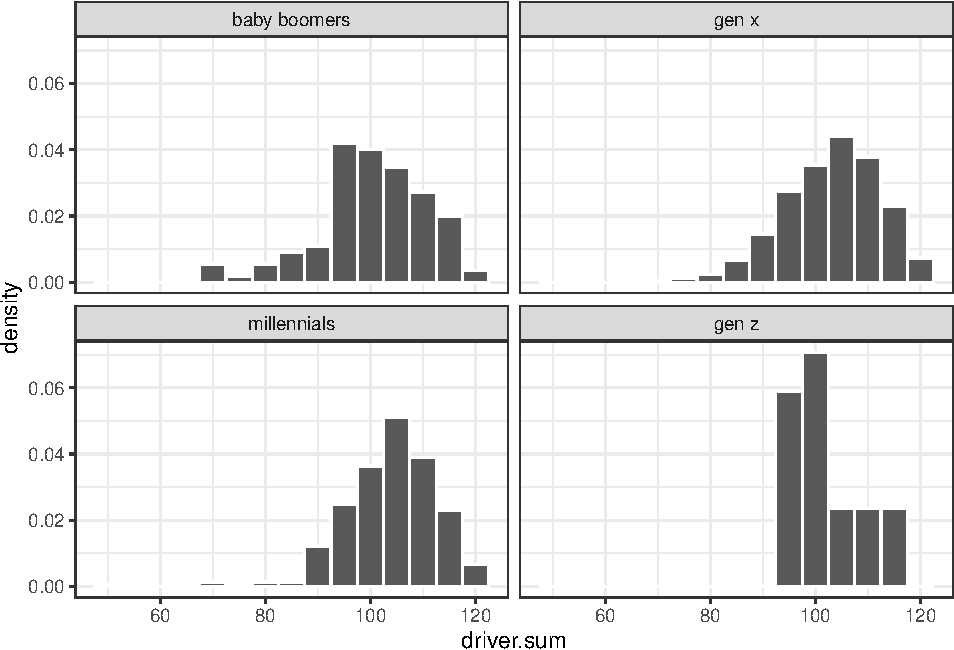
\includegraphics{R-for-social-research-and-business-analytics_files/figure-latex/unnamed-chunk-43-1.pdf}

Faceting functions in ggplot2 are very flexible and allow us to explore any kind of grouping by one or more categorical variable. For example, we may want to look at intersections of generations and genders, that is, generation-gender groups. With \texttt{facet\_grid()}, we can have a neat matrix with generations as rows and genders as columns, each cell being a generation-gender combination:

\begin{Shaded}
\begin{Highlighting}[]
\CommentTok{\# For simplicity, let\textquotesingle{}s first subset the data to just Male and Female genders.}
\NormalTok{data.mf }\OtherTok{\textless{}{-}}\NormalTok{ data }\SpecialCharTok{|\textgreater{}} 
  \FunctionTok{filter}\NormalTok{(gender }\SpecialCharTok{\%in\%} \FunctionTok{c}\NormalTok{(}\StringTok{"Donna"}\NormalTok{, }\StringTok{"Uomo"}\NormalTok{))}

\CommentTok{\# Now plot}
\FunctionTok{ggplot}\NormalTok{(}\AttributeTok{data =}\NormalTok{ data.mf) }\SpecialCharTok{+}
  \FunctionTok{geom\_histogram}\NormalTok{(}\FunctionTok{aes}\NormalTok{(}\AttributeTok{x =}\NormalTok{ driver.sum, }\AttributeTok{y =} \FunctionTok{after\_stat}\NormalTok{(density)), }\AttributeTok{binwidth =} \DecValTok{5}\NormalTok{, }\AttributeTok{color =} \StringTok{"white"}\NormalTok{) }\SpecialCharTok{+}
  \FunctionTok{facet\_grid}\NormalTok{(gen }\SpecialCharTok{\textasciitilde{}}\NormalTok{ gender) }\SpecialCharTok{+}
  \FunctionTok{theme\_bw}\NormalTok{()}
\end{Highlighting}
\end{Shaded}

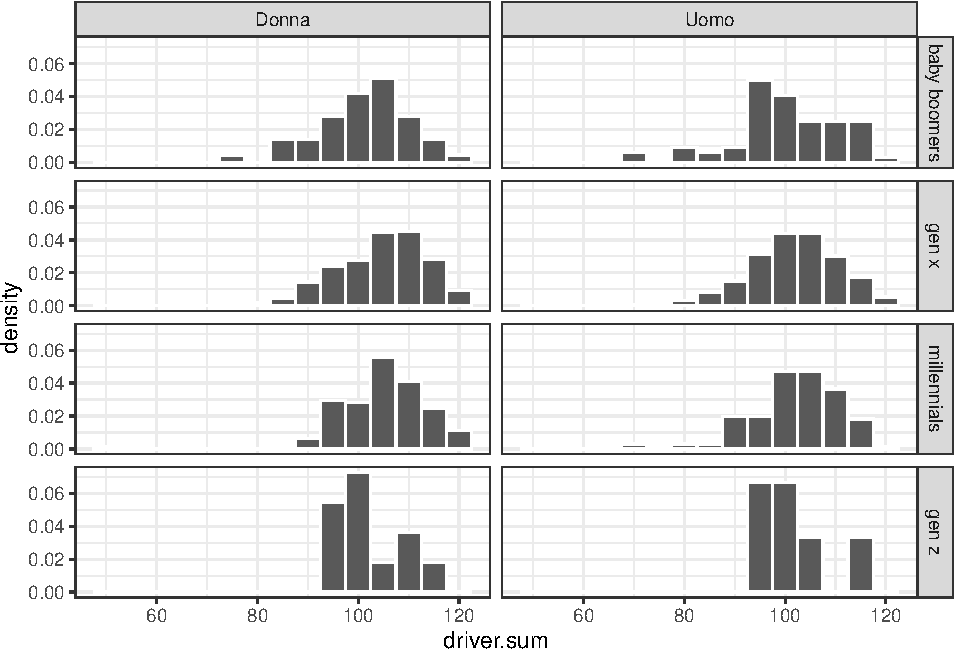
\includegraphics{R-for-social-research-and-business-analytics_files/figure-latex/unnamed-chunk-44-1.pdf}

\hypertarget{reproducible}{%
\chapter{Creating reproducible reports}\label{reproducible}}

  \bibliography{book.bib,packages.bib}

\end{document}
